\documentclass[11pt,a4paper,oneside]{report}             % Single-side
%\documentclass[11pt,a4paper,twoside,openright]{report}  % Duplex

%\PassOptionsToPackage{chapternumber=Huordinal}{magyar.ldf}
\usepackage{t1enc}
\usepackage[utf8x]{inputenc}
\usepackage{lmodern}
%\usepackage{newunicodechar} 
%\DeclareUnicodeCharacter{FFFD}{?????}

\usepackage{amsmath}
\usepackage{amssymb}
\usepackage{enumerate}
\usepackage[thmmarks,amsmath]{ntheorem}
\usepackage{graphics}
\usepackage{epsfig}
\usepackage{listingsutf8}
\usepackage{color}
%\usepackage{fancyhdr}
\usepackage{lastpage}
\usepackage{anysize}
\usepackage[magyar, british]{babel}
\usepackage{sectsty}
\usepackage{setspace}  % Ettol a tablazatok, abrak, labjegyzetek maradnak 1-es sorkozzel!
\usepackage[hang]{caption}
\usepackage{hyperref}
\usepackage{xcolor}
\usepackage{makecell}

%--------------------------------------------------------------------------------------
% Main variables
%--------------------------------------------------------------------------------------
\newcommand{\vikszerzo}{Orsolya Deák}
\newcommand{\vikkonzulens}{Gábor Simon}
\newcommand{\vikcim}{Developing a Reservation System on Azure Serverless Platform}
\newcommand{\viktanszek}{Department of Automation and Applied Informatics}
\newcommand{\vikdoktipus}{Bachelor's Thesis}
\newcommand{\vikdepartmentr}{Bódis-Szomorú András}

%--------------------------------------------------------------------------------------
% Page layout setup
%--------------------------------------------------------------------------------------
% we need to redefine the pagestyle plain
% another possibility is to use the body of this command without \fancypagestyle
% and use \pagestyle{fancy} but in that case the special pages
% (like the ToC, the References, and the Chapter pages)remain in plane style

\pagestyle{plain}
\setlength{\parindent}{0pt} % áttekinthetőbb, angol nyelvű dokumentumokban jellemző
\setlength{\parskip}{8pt plus 3pt minus 3pt} % áttekinthetőbb, angol nyelvű dokumentumokban jellemző
%\setlength{\parindent}{12pt} % magyar nyelvű dokumentumokban jellemző
%\setlength{\parskip}{0pt}    % magyar nyelvű dokumentumokban jellemző

\marginsize{35mm}{25mm}{15mm}{15mm} % anysize package
\setcounter{secnumdepth}{0}
\sectionfont{\large\upshape\bfseries}
\setcounter{secnumdepth}{2}
\singlespacing
\frenchspacing

%--------------------------------------------------------------------------------------
%	Setup hyperref package
%--------------------------------------------------------------------------------------
\hypersetup{
    bookmarks=true,            % show bookmarks bar?
    unicode=false,             % non-Latin characters in Acrobat’s bookmarks
    pdftitle={\vikcim},        % title
    pdfauthor={\vikszerzo},    % author
    pdfsubject={\vikdoktipus}, % subject of the document
    pdfcreator={\vikszerzo},   % creator of the document
    pdfproducer={Producer},    % producer of the document
    pdfkeywords={keywords},    % list of keywords
    pdfnewwindow=true,         % links in new window
    colorlinks=true,           % false: boxed links; true: colored links
    linkcolor=black,           % color of internal links
    citecolor=black,           % color of links to bibliography
    filecolor=black,           % color of file links
    urlcolor=black             % color of external links
}

%--------------------------------------------------------------------------------------
% Set up listings
%--------------------------------------------------------------------------------------
\lstset{
	basicstyle=\scriptsize\ttfamily, % print whole listing small
	keywordstyle=\color{black}\bfseries\underbar, % underlined bold black keywords
	identifierstyle=, 					% nothing happens
	commentstyle=\color{white}, % white comments
	stringstyle=\scriptsize\sffamily, 			% typewriter type for strings
	showstringspaces=false,     % no special string spaces
	aboveskip=3pt,
	belowskip=3pt,
	columns=fixed,
	backgroundcolor=\color{lightgray},
	literate={ö}{{\"{o}}}1 {Ö}{{\"{O}}}1 {ü}{{\"{u}}}1 {Ü}{{\"{u}}}1 {ó}{{\'{o}}}1 {Ó}{{\'{O}}}1 {ő}{{\H{o}}}1 {Ő}{{\H{O}}}1 {ú}{{\'{u}}}1 {Ú}{{\'{U}}}1 {é}{{\'{e}}}1 {É}{{\'{E}}}1 {á}{{\'{a}}}1 {Á}{{\'{A}}}1 {ű}{{\H{u}}}1 {Ű}{{\H{U}}}1 {í}{{\'{i}}}1 {Í}{{\'{I}}}1
} 		
\def\lstlistingname{lista}	

%--------------------------------------------------------------------------------------
%	Some new commands and declarations
%--------------------------------------------------------------------------------------
\newcommand{\code}[1]{{\upshape\ttfamily\scriptsize\indent #1}}

% define references
\newcommand{\figref}[1]{\ref{fig:#1}.}
\renewcommand{\eqref}[1]{(\ref{eq:#1})}
\newcommand{\listref}[1]{\ref{listing:#1}.}
\newcommand{\sectref}[1]{\ref{sect:#1}}
\newcommand{\tabref}[1]{\ref{tab:#1}.}

\DeclareMathOperator*{\argmax}{arg\,max}
%\DeclareMathOperator*[1]{\floor}{arg\,max}
\DeclareMathOperator{\sign}{sgn}
\DeclareMathOperator{\rot}{rot}
\definecolor{lightgray}{rgb}{0.95,0.95,0.95}

\author{\vikszerzo}
\title{\vikcim}
\includeonly{
	%guideline,%
	%project,%
	titlepage,%
	declaration,%
	abstract,%
	introduction,%
	chapter1,%
	chapter2,%
	chapter3,%
	chapter4,%
	chapter5,%
	chapter6,%
	chapter7,%
	acknowledgement,%
	appendices,%
}
%--------------------------------------------------------------------------------------
%	Setup captions
%--------------------------------------------------------------------------------------
\captionsetup[figure]{
%labelsep=none,
%font={footnotesize,it},
%justification=justified,
width=.75\textwidth,
aboveskip=10pt}

\renewcommand{\captionlabelfont}{\small\bf}
\renewcommand{\captionfont}{\footnotesize\it}


\hyphenation{meg-kí-sé-rel-tem össze-mér-he-tő}


%--------------------------------------------------------------------------------------
% Table of contents and the main text
%--------------------------------------------------------------------------------------
\begin{document}

\pagestyle{empty}
%%--------------------------------------------------------------------------------------
% Rovid formai es tartalmi tajekoztato
%--------------------------------------------------------------------------------------

\footnotesize
\begin{center}
\large
\textbf{\Large Általános információk, a diplomaterv szerkezete}\\
\end{center}

A diplomaterv szerkezete a BME Villamosmérnöki és Informatikai Karán:
\begin{enumerate}
\item	Diplomaterv feladatkiírás
\item	Címoldal
\item	Tartalomjegyzék
\item	A diplomatervező nyilatkozata az önálló munkáról és az elektronikus adatok kezeléséről
\item	Tartalmi összefoglaló magyarul és angolul
\item	Bevezetés: a feladat értelmezése, a tervezés célja, a feladat indokoltsága, a diplomaterv felépítésének rövid összefoglalása
\item	A feladatkiírás pontosítása és részletes elemzése
\item	Előzmények (irodalomkutatás, hasonló alkotások), az ezekből levonható következtetések
\item	A tervezés részletes leírása, a döntési lehetőségek értékelése és a választott megoldások indoklása
\item	A megtervezett műszaki alkotás értékelése, kritikai elemzése, továbbfejlesztési lehetőségek
\item	Esetleges köszönetnyilvánítások
\item	Részletes és pontos irodalomjegyzék
\item	Függelék(ek)
\end{enumerate}

Felhasználható a következő oldaltól kezdődő \LaTeX-Diplomaterv sablon dokumentum tartalma. 

A diplomaterv szabványos méretű A4-es lapokra kerüljön. Az oldalak tükörmargóval készüljenek (mindenhol 2.5cm, baloldalon 1cm-es kötéssel). Az alapértelmezett betűkészlet a 12 pontos Times New Roman, másfeles sorközzel.

Minden oldalon - az első négy szerkezeti elem kivételével - szerepelnie kell az oldalszámnak.

A fejezeteket decimális beosztással kell ellátni. Az ábrákat a megfelelő helyre be kell illeszteni, fejezetenként decimális számmal és kifejező címmel kell ellátni. A fejezeteket decimális aláosztással számozzuk, maximálisan 3 aláosztás mélységben (pl. 2.3.4.1.). Az ábrákat, táblázatokat és képleteket célszerű fejezetenként külön számozni (pl. 2.4. ábra, 4.2 táblázat vagy képletnél (3.2)). A fejezetcímeket igazítsuk balra, a normál szövegnél viszont használjunk sorkiegyenlítést. Az ábrákat, táblázatokat és a hozzájuk tartozó címet igazítsuk középre. A cím a jelölt rész alatt helyezkedjen el.

A képeket lehetőleg rajzoló programmal készítsék el, az egyenleteket egyenlet-szerkesztő segítségével írják le (A \LaTeX~ehhez kézenfekvő megoldásokat nyújt).

Az irodalomjegyzék szövegközi hivatkozása történhet a Harvard-rendszerben (a szerző és az évszám megadásával) vagy sorszámozva. A teljes lista névsor szerinti sorrendben a szöveg végén szerepeljen (sorszámozott irodalmi hivatkozások esetén hivatkozási sorrendben). A szakirodalmi források címeit azonban mindig az eredeti nyelven kell megadni, esetleg zárójelben a fordítással. A listában szereplő valamennyi publikációra hivatkozni kell a szövegben (a \LaTeX-sablon a Bib\TeX~segítségével mindezt automatikusan kezeli). Minden publikáció a szerzők után a következő adatok szerepelnek: folyóirat cikkeknél a pontos cím, a folyóirat címe, évfolyam, szám, oldalszám tól-ig. A folyóirat címeket csak akkor rövidítsük, ha azok nagyon közismertek vagy nagyon hosszúak. Internet hivatkozások megadásakor fontos, hogy az elérési út előtt megadjuk az oldal tulajdonosát és tartalmát (mivel a link egy idő után akár elérhetetlenné is válhat), valamint az elérés időpontját.

\vspace{5mm}
Fontos:
\begin{itemize}
	\item A szakdolgozat készítő / diplomatervező nyilatkozata (a jelen sablonban szereplő szövegtartalommal) kötelező előírás Karunkon ennek hiányában a szakdolgozat/diplomaterv nem bírálható és nem védhető !
	\item Mind a dolgozat, mind a melléklet maximálisan 15 MB méretű lehet !
\end{itemize}

\vspace{5mm}
\begin{center}
Jó munkát, sikeres szakdolgozat készítést ill. diplomatervezést kívánunk !
\end{center}

\normalsize

%%--------------------------------------------------------------------------------------
% Feladatkiiras (a tanszeken atveheto, kinyomtatott valtozat)
%--------------------------------------------------------------------------------------
\clearpage
\begin{center}
\large
\textbf{FELADATKIÍRÁS}\\
\end{center}

A feladatkiírást a tanszéki adminisztrációban lehet átvenni, és a leadott munkába eredeti, tanszéki pecséttel ellátott és a tanszékvezető által aláírt lapot kell belefűzni (ezen oldal \emph{helyett}, ez az oldal csak útmutatás). Az elektronikusan feltöltött dolgozatban már nem kell beleszerkeszteni ezt a feladatkiírást.





%--------------------------------------------------------------------------------------
%	The title page
%--------------------------------------------------------------------------------------
\begin{titlepage}
\begin{center}

\includegraphics[width=60mm,keepaspectratio]{figures/BMElogo.png}\\
\vspace{0.3cm}
\textbf{Budapest University of Technology and Economics}\\
\textmd{Faculty of Electrical Engineering and Informatics}\\
\textmd{\viktanszek}\\[5cm]

\vspace{0.4cm}
{\huge \bfseries \vikcim}\\[0.8cm]
\vspace{0.5cm}
\textsc{\Large \vikdoktipus}\\[4cm]

\begin{tabular}{cc}
 \makebox[7cm]{\emph{Author}} & \makebox[7cm]{\emph{Advisor}} \\
 \makebox[7cm]{\vikszerzo} & \makebox[7cm]{\vikkonzulens}
\end{tabular}

\vfill
{\large \today}
\end{center}
\end{titlepage}




\pagestyle{plain}
\pagenumbering{roman}
%----------------------------------------------------------------------------
% Abstract in hungarian
%----------------------------------------------------------------------------
\chapter*{Kivonat}\addcontentsline{toc}{chapter}{Kivonat}

Szakdolgozatom célja egy éttermi foglaló rendszert megvalósító serverless alkalmazás implementálása volt valamely felhőszolgáltó erőforrásainak felhasználásával. Továbbá megkíséreltem felmérni, hogy egy serverless alkalmazás teljesítménye és fejlesztői élménye összemérhető-e a hagyományos megközelítésével. Ehhez a Microsoft Azure felhőjét, ezen belül kliensoldalon az Azure Static Web Apps szolgáltatást használtam Angular keretrendszerrel, Azure Function Appot szerveroldalon és Cosmos DB-t az alkalmazás adatainak tárolására. A kész alkalmazáson terheléses tesztet végeztem, amelynek eredményei arra engedtek következtetni, hogy az alkalmazás a lekérdezések mennyiségének megfelelően skálázódik, alátámasztva ezzel azt a feltevést, hogy a szerverek kezelését a serverless rendszer önmaga megoldja.
Végül kiértékeltem a megoldást és arra a következtetésre jutottam, hogy a serverless megközelítés a programozó eszköztárának hasznos részét képezi. 
\vfill

%----------------------------------------------------------------------------
% Abstract in english
%----------------------------------------------------------------------------
\chapter*{Abstract}\addcontentsline{toc}{chapter}{Abstract}

In this thesis I aimed to implement a serverless application on a cloud provider's service, which accomplishes a restaurant reservation system. I also attempted to measure whether a serverless app's performance and coding experience can be as good as the conventional approach. 
For this, I used Microsoft's Azure cloud, more precisely Azure Static Web Apps with Angular framework on the frontend, Azure Function Apps on the server side and Cosmos DB as data storage.
I did loadtesting on the finished application and the results showed that it scaled according to the request volume, meaning it indeed has the advantage of removing the need to manually manage servers.
Finally, I evaluated the solution and came to the conclusion that serverless is a useful approach, which has its place in a programmer's toolbox.
\vfill


\tableofcontents\vfill
%--------------------------------------------------------------------------------------
% Nyilatkozat
%--------------------------------------------------------------------------------------
\begin{center}
\large
\textbf{HALLGATÓI NYILATKOZAT}\\
\end{center}

Alulírott \emph{Deák Orsolya}, szigorló hallgató kijelentem, hogy ezt a szakdolgozatot meg nem engedett segítség nélkül, saját magam készítettem, csak a megadott forrásokat (szakirodalom, eszközök stb.) használtam fel. Minden olyan részt, melyet szó szerint, vagy azonos értelemben, de átfogalmazva más forrásból átvettem, egyértelműen, a forrás megadásával megjelöltem.

Hozzájárulok, hogy a jelen munkám alapadatait (szerző(k), cím, angol és magyar nyelvű tartalmi kivonat, készítés éve, konzulens(ek) neve) a BME VIK nyilvánosan hozzáférhető elektronikus formában, a munka teljes szövegét pedig az egyetem belső hálózatán keresztül (vagy autentikált felhasználók számára) közzétegye. Kijelentem, hogy a benyújtott munka és annak elektronikus verziója megegyezik. Dékáni engedéllyel titkosított diplomatervek esetén a dolgozat szövege csak 3 év eltelte után válik hozzáférhetővé.

\begin{flushleft}
\vspace*{1cm}
Budapest, 2022. December 9.
\end{flushleft}

\begin{flushright}
 \vspace*{1cm}
 \makebox[7cm]{\rule{6cm}{.4pt}}\\
 \makebox[7cm]{\emph{Deák Orsolya}}\\
 \makebox[7cm]{hallgató}
\end{flushright}
\thispagestyle{empty}

\vfill
\clearpage
\thispagestyle{empty} % an empty page



\pagenumbering{arabic}

%----------------------------------------------------------------------------
\chapter{Introduction}\label{Introduction}
%----------------------------------------------------------------------------

Cloud solutions are nowadays more and more prevalent. Big tech companies like Microsoft, Google or Amazon are constantly improving their services, which means that they think this technology will be present for a long period of time. Perhaps they are correct because cloud services can solve multiple problems if implemented right.

But what do we mean by cloud solutions \cite{CloudDef}? In a nutshell, it's like a rental company just for IT resources, accessed through the internet. Conventionally they fall into three categories: 
\begin{itemize}
	\item Infrastructure-as-a-Service~(IaaS),
	\item Platform-as-a-Service~(PaaS),
	\item Software-as-a-Service~(SaaS).
\end{itemize}

IaaS means that the cloud provider lets users use their advanced infrastructure, so they don't have to set up and maintain a local server on their site, all of this is handled by the provider. According to \cite{AzurePatterns} application monitoring, package management, and server backups remain the user's responsibility.
In case of PaaS all of these are handled by the cloud provider. Here a software platform or framework is provided to the users, which is suitable for e.g.\ application development without the often complex maintenance needs. Users still have to take care of the server scaling.
Finally, SaaS means one can connect to and use a software without local installation.

These categories are not comprehensive, there are others as well, but I would like to mention just one more.
\begin{itemize}
	\item Function-as-a-Service (FaaS)~\cite{FaaS}
\end{itemize}
In this case the developer deploys the code to the service, which will run it automatically, when called.  

Serverless is a more abstract version of PaaS~\cite{ServerlessDef}. Here the users have the opportunity to flexibly use a provider's resources and only paying for the amount that was really in use. If there is a greater demand for the resources, e.g.\ on a Black Friday sale, when a lot more people would like to access the user's website, then the resources scale automatically, so there will be no service outage. Providers also guarantee threat prevention and detection technologies. The name suggests that we don't need to own a server: we will use the ones of the provider.

One can argue that with these solutions the user only gets a limited amount of configuration options and can not peek into the actual code of the used software. These are valid observations and businesses should think about on what level are they willing to rely on a cloud provider. However they also result in more reliable and a lot more flexible services, which can spare a headache and even money for the businesses who decide to use them.

Why did we mention all of this? Because these are the solutions that were used in this project.

My thesis' goal was to develop a reservation platform for restaurants, where these restaurants can be registered so guests can find them, order food and book tables for a chosen time slot. 
This problem could have been solved without the serverless approach, but I decided on it because of multiple reasons. The user amount can be very volatile. First of all because it is a self-registration system, so as it would be more and more known the more users would want to register and use the platform simultaneously. Secondly, because the mood and possibility for eating out may rapidly change as we have seen in the previous years. Just between weekdays and weekends or holidays the demand of eating out can vary greatly. In this aspect, a serverless solution can help us out. Last but not least, I wanted to try and learn a new approach.

The structure of this thesis will be the following: 
 \begin{itemize}
 	\item Chapter \ref{Introduction}: Introduction
	\item Chapter \ref{Ch1}: Here I will analyze the software requirements. 
	\item Chapter \ref{Ch2}: We will look at our software architecture options.
	\item Chapter \ref{Ch3}: We discuss the created user interface and the frontend of the application.
	\item Chapter \ref{Ch4}: I write in detail about the used Azure components.
	\item Chapter \ref{Ch5}: I talk about how the solution could be improved.
	\item Chapter \ref{Ch6}: We take a look at the load testing results and evaluate whether or not serverless lives up to our expectations.
	\item Chapter \ref{Ch7}: Finally, I summarize my experiences.
\end{itemize}
%----------------------------------------------------------------------------
\chapter{Application expectations}\label{Ch1}
%----------------------------------------------------------------------------
In this section I will shortly discuss the chosen problem, so that the reader can understand the main goal and context of the following chapters. We will take a look at the user story, then break it down to use cases. At the second part of the chapter we will compose three user flows based on them.
%----------------------------------------------------------------------------
\section{User Story}
%----------------------------------------------------------------------------

Under real life circumstances the developer gets a vague and not at all professional description of what the job would be. I wanted to simulate this because it would give us a compact description of the problem. The user story I created for myself in this instance reads as follows: 

 \emph{
 	We need an application where restaurants can be registered, upload their offers and other useful data like opening hours. Guests can also log in and order food for takeaway or dine in. In the second case let them choose a table at the restaurant. They should also provide information about when they want to take it or eat the dish, so they can be served minutes after arrival. Guests pay in advance right after order, so there will be fewer cases of unclaimed orders. Also they don't have to wait for payment on site. Guests can give feedback on their experience.
 } 

For simplicity's sake from now on I will call this app \emph{Allegro}.

%----------------------------------------------------------------------------
\section{Use Cases}
%----------------------------------------------------------------------------
 As a next step, I defined the use cases based on the user story and created the following use case diagram (Figure \figref{UseCaseDiagram}). I will give a short summary below. 
 
We have three potential Actors: 

\begin{itemize}
	\item \verb+Anonymous Users+,
	\item \verb+Guests+, who are logged in users without a restaurant connected to them,
	\item \verb+Restaurants+, who are logged in users with a restaurant.
\end{itemize}

 \begin{figure}[!ht]
	\centering
	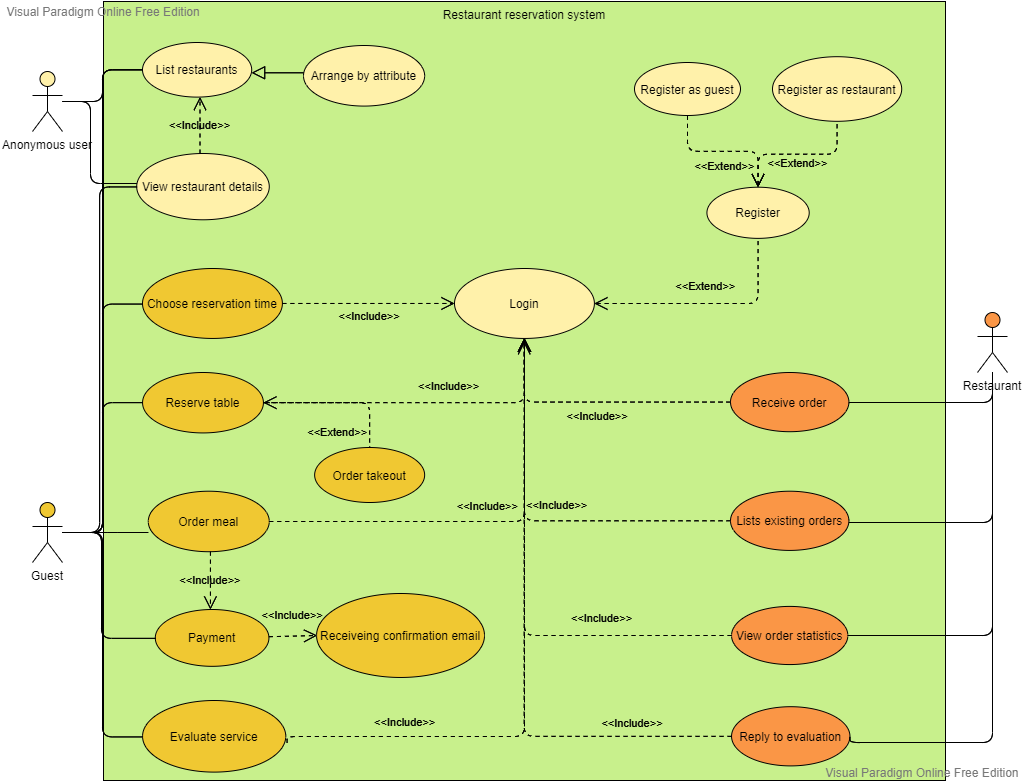
\includegraphics[width=150mm, keepaspectratio]{figures/UseCaseDiagram}
	\caption{Use Case Diagram} 
	\label{fig:UseCaseDiagram}
\end{figure}

\verb+Anonymous Users+ have the options to list existing restaurants, view them one by one in a detailed view, log in if they already have an account or create a guest or restaurant account. 

Someone with a \verb+Guest+ account can walk through the food ordering process which includes reserving table at a given restaurant for a given date and time, ordering meal and paying for these. They can also evaluate the restaurant they ordered at.

\verb+Restaurants+ will have the ability to receive orders, list them, view their statistics and write a reply to guest evaluations.

The full list of the created use cases can be found in the Appendix under \ref{usecases}.

%----------------------------------------------------------------------------
\section{User Flows}
%----------------------------------------------------------------------------

After the use cases were finished, I could move to figuring out how the users were expected to interact with the application. As we see on the use case diagram, I defined three roles. Here I'll give a short description of each.
%----------------------------------------------------------------------------
\subsection{Anonymous User}\label{AnonUserflow}
%----------------------------------------------------------------------------
 Based on the use cases, I thought a restaurant list would be a good entry point for the users. From there it should be an option to choose a specific restaurant and navigate to its details page. The anonymous user's use cases are, in this way, properly handled, so at this point there should be a login option which diverges to the guest and the restaurant user flow. See a graphic explanation at Figure \figref{UIsAnon}
\begin{figure}[!ht]
	\centering
	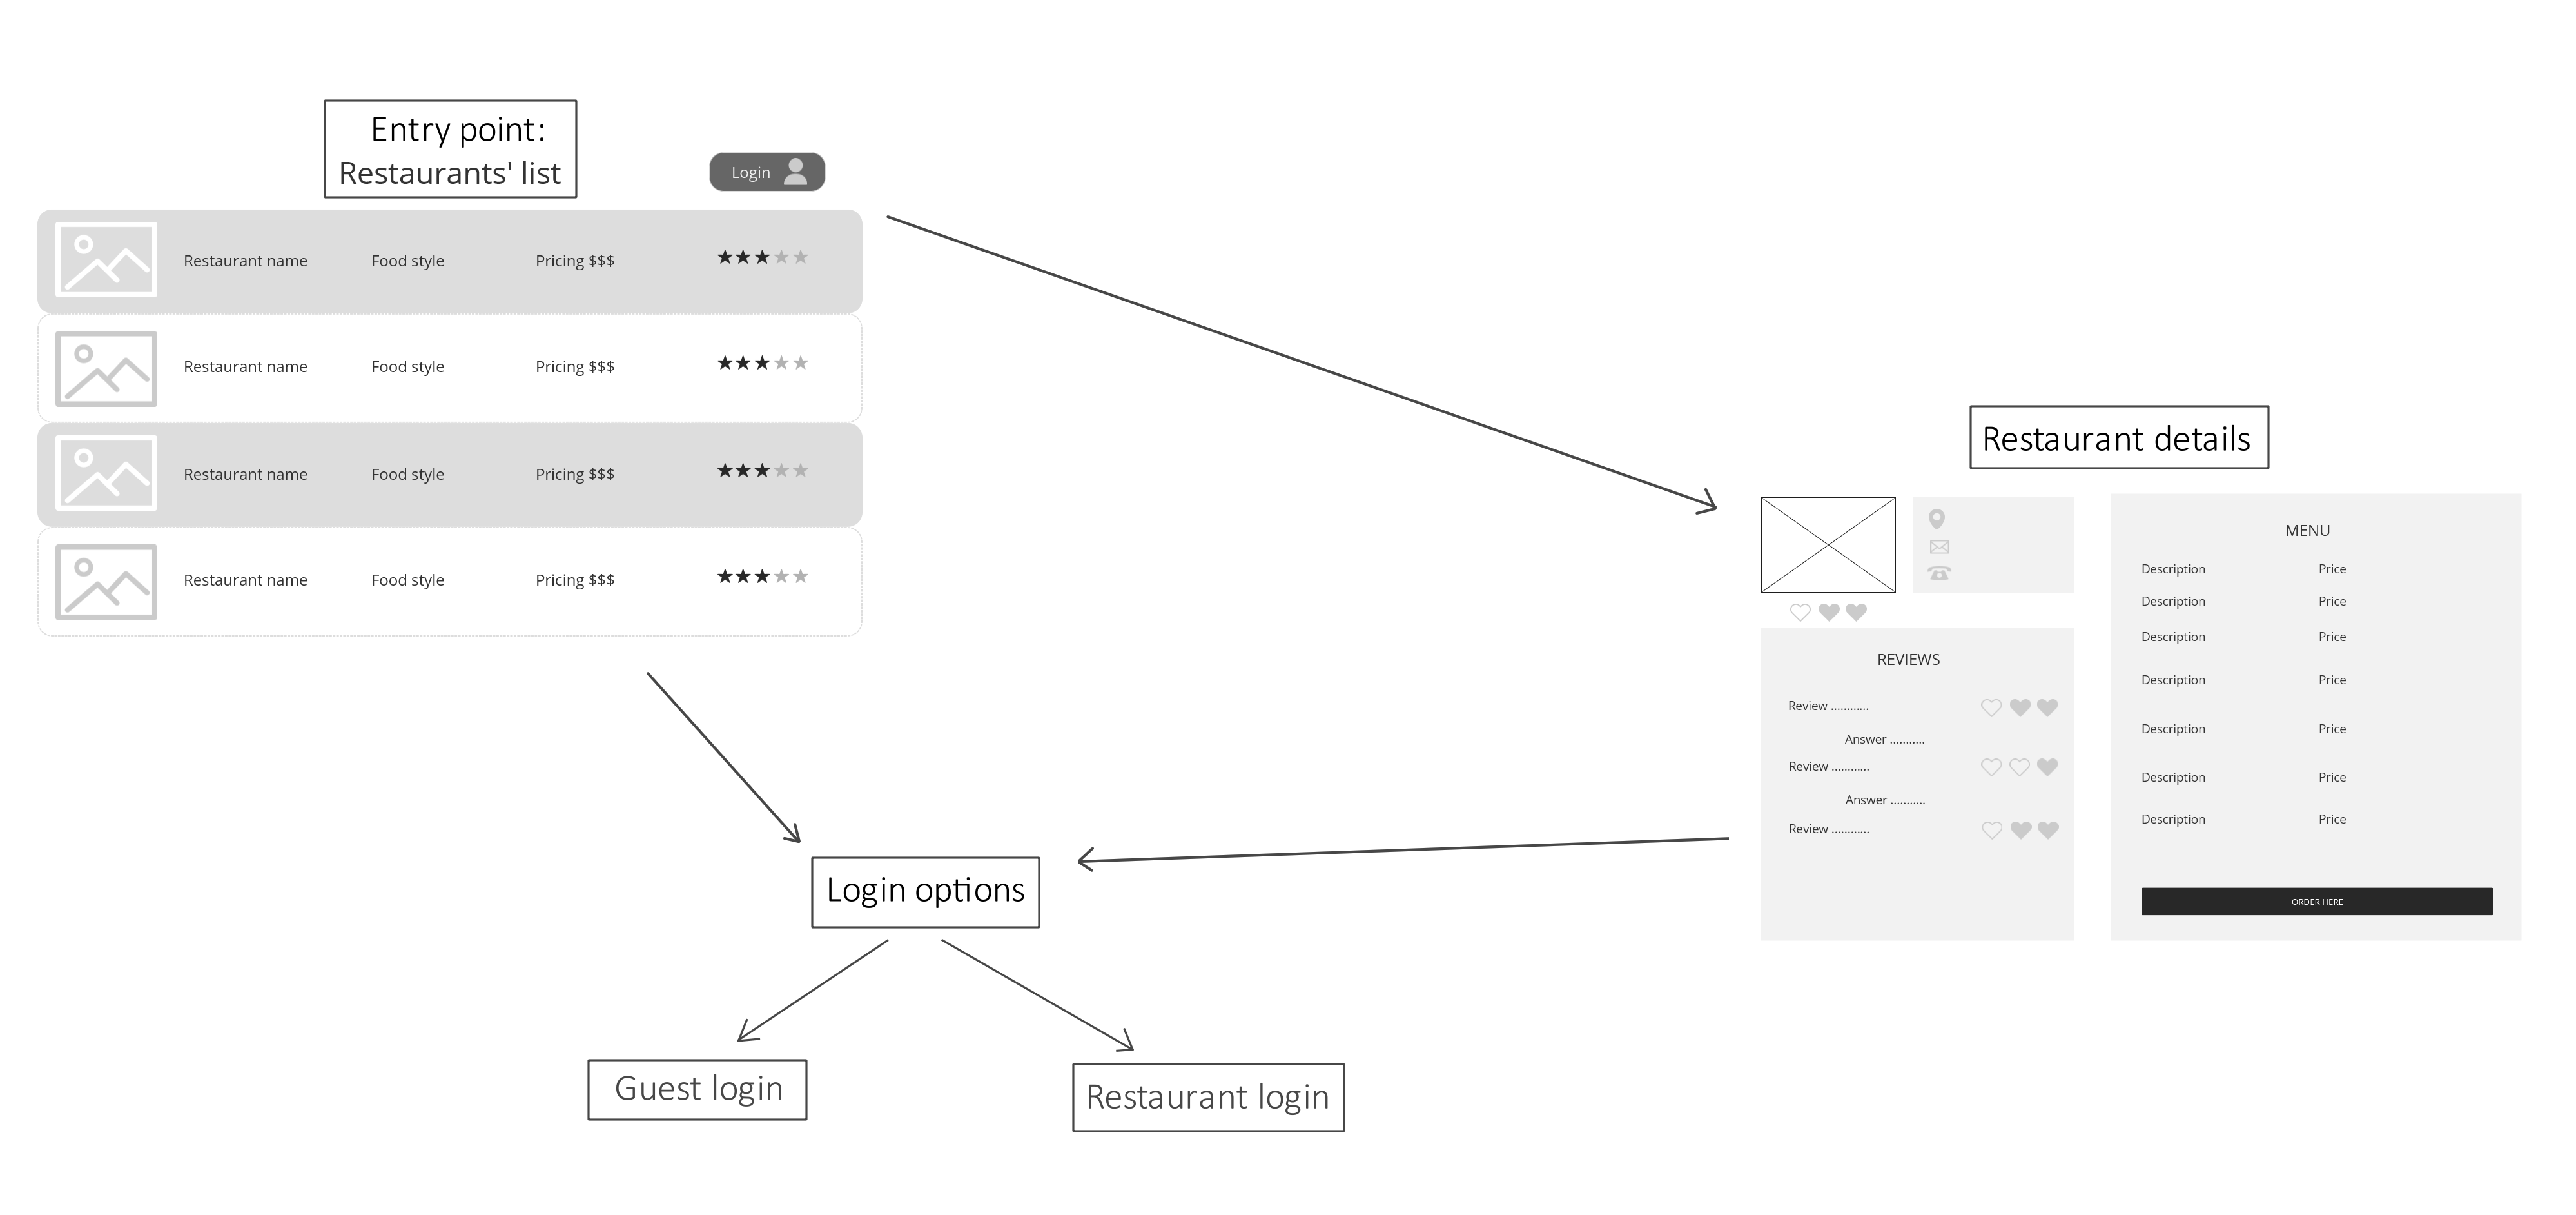
\includegraphics[width=150mm, keepaspectratio]{figures/UIsAnon.png}
	\caption{Anonymous user's user flow} 
	\label{fig:UIsAnon}
\end{figure}
%----------------------------------------------------------------------------
\subsection{Guest}\label{GuestUserflow}
%----------------------------------------------------------------------------
At the login page there should be an option to sign in or register as a guest or to do the same as a restaurant owner. Following the use case diagram, a guest can choose a restaurant to order from, so after signing in he should start his journey at the restaurants' list page then to the details page and then navigate to an order site provided he is, indeed, authenticated. Alternatively, in case we allow to start the order process as an anonymous user, the user should be prompted to log in, then redirected to the chosen restaurant's order page. Here he should be able to book a table or order takeaway and save the date and time. Next, he can navigate to the menu and pick the wished dishes. Afterwards, the order details can be checked and modified and finally the payment can be done. Here we would like to send e-mails to the guest about the successful payment and the order details. Finally, the guest can send a feedback about his experiences. See Figure \figref{UIsGuest}
\begin{figure}[!ht]
	\centering
	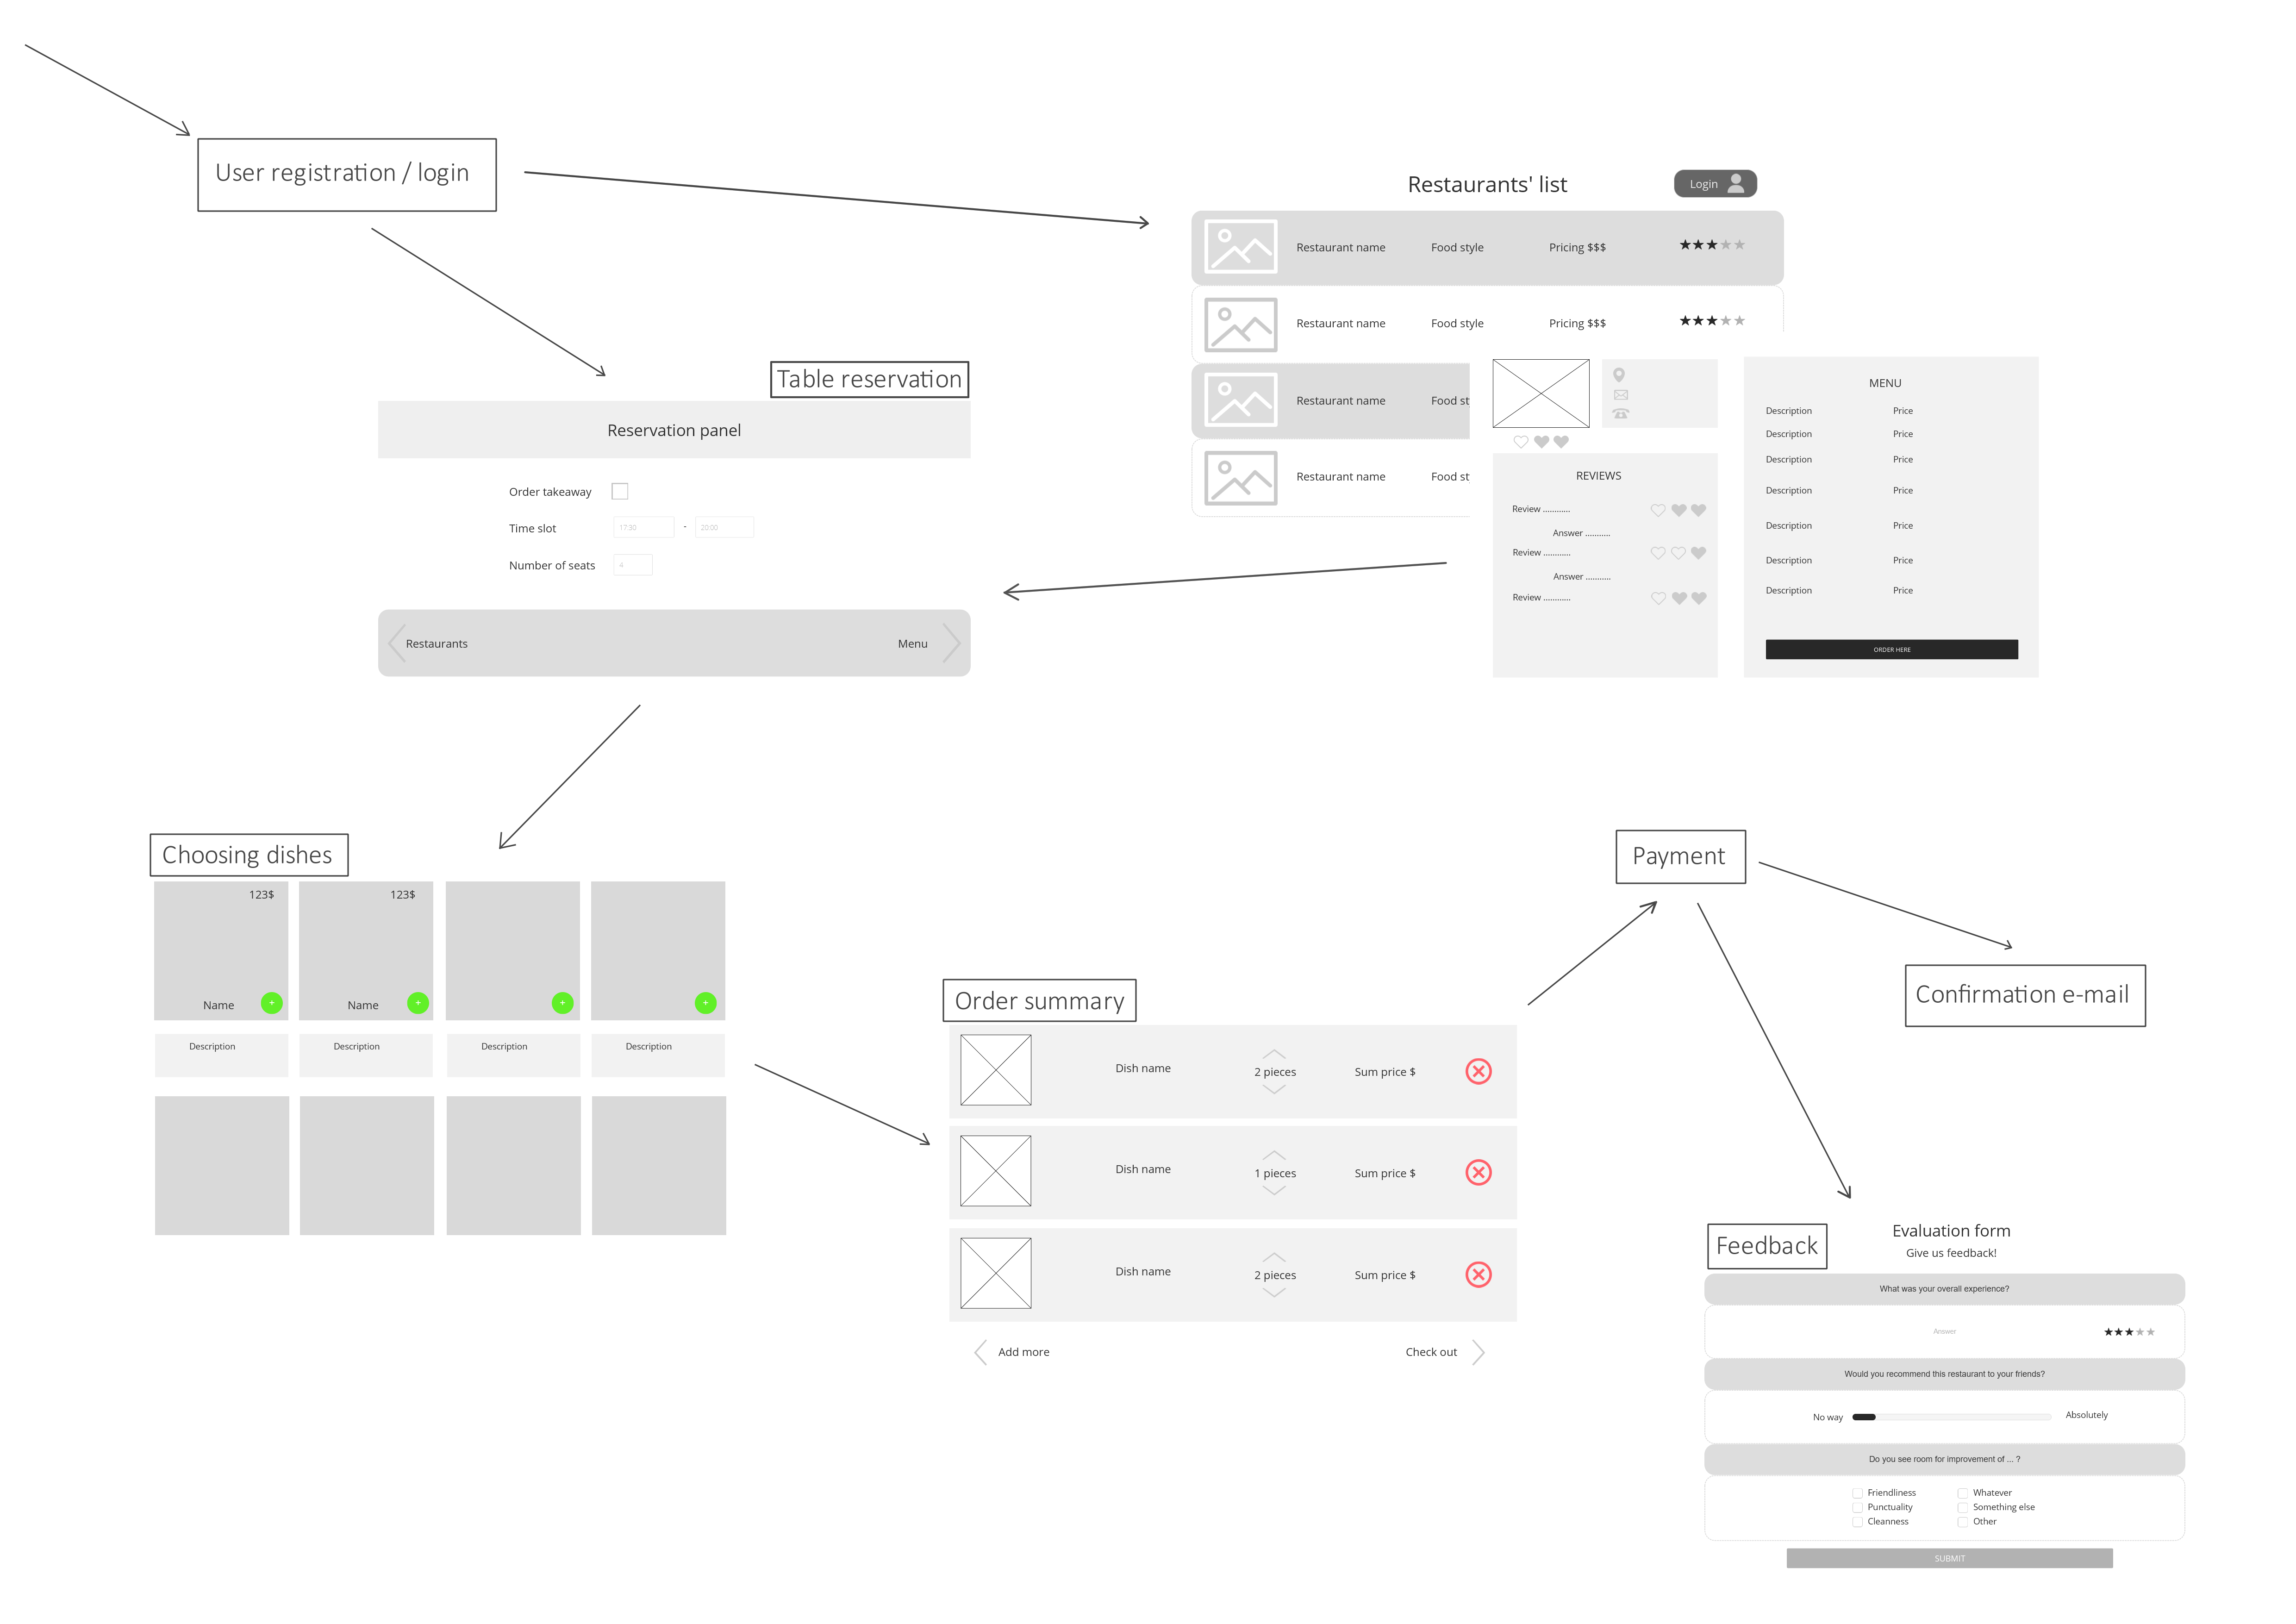
\includegraphics[width=150mm, keepaspectratio]{figures/UIsGuest.png}
	\caption{Guest's user flow} 
	\label{fig:UIsGuest}
\end{figure}
%----------------------------------------------------------------------------
\subsection{Restaurant}\label{RestaurantUserflow}
%----------------------------------------------------------------------------
If one decides to create a new restaurant, he has to register through three steps. First, the basic data should be collected e.g.\ contact information. Then the restaurant user can add the menu and finally the table information, from which the guests will choose from. If the registration was successful, the restaurant user can log in and will be redirected to a dashboard, where the restaurant's orders and reviews will be displayed. From here he can navigate to data modification pages and can answer to the reviews. See Figure \figref{UIsRestaurant}
\begin{figure}[!ht]
	\centering
	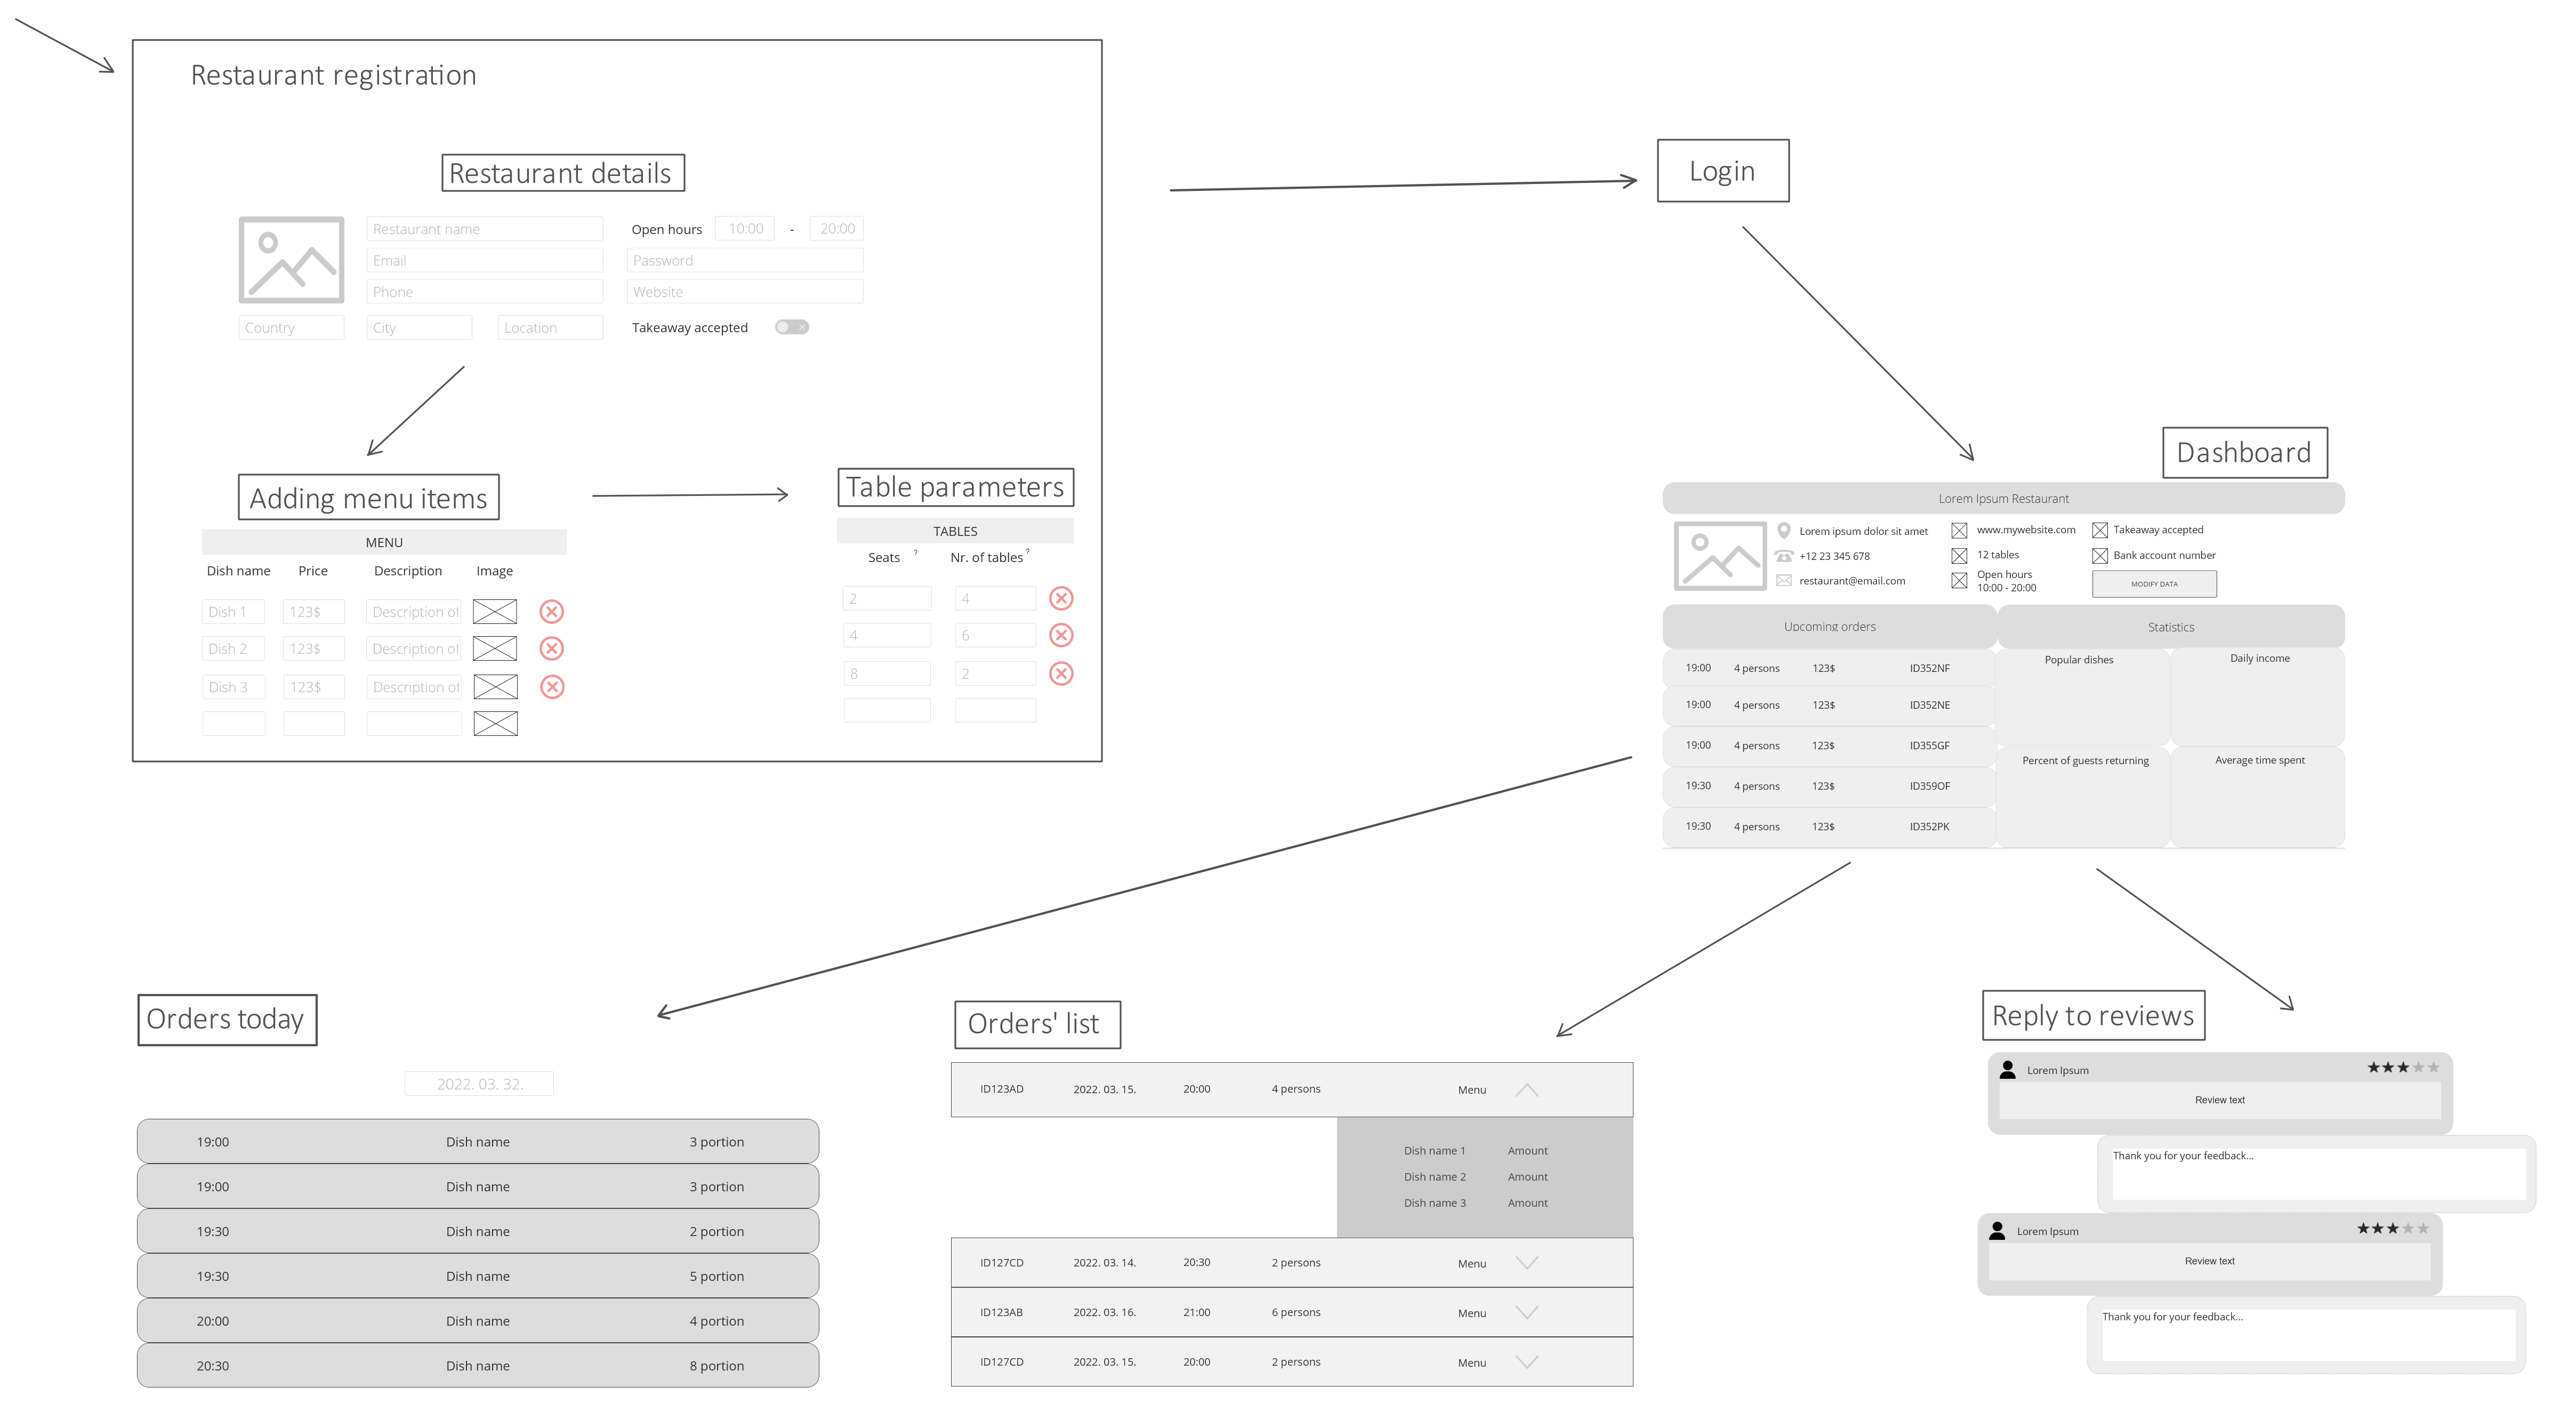
\includegraphics[width=150mm, keepaspectratio]{figures/UIsRestaurant.png}
	\caption{Restaurant's user flow} 
	\label{fig:UIsRestaurant}
\end{figure}
%----------------------------------------------------------------------------
\chapter{Software Architecture}\label{Ch2}
%----------------------------------------------------------------------------
Now that we have a basic understanding of the requirements, the architecture may be chosen. 

%----------------------------------------------------------------------------
\section{Serverless Architecture}
%----------------------------------------------------------------------------

As the vigilant reader probably noticed already, I will be developing a serverless application \cite{AzurePatterns}. I will rely on the things I already discussed in the Introduction  (Chapter~\ref{Introduction}). There are a few things to take into account.  This allows me not to care too much about where and how my application will be running. I don't have to configure a server or worry about whether or not I will have enough storage space locally.

There are multiple options to choose from if one would like to start working with serverless \cite{ServerlessPlatforms}. The most popular cloud computing platforms are Amazon Web Services \cite{AWS}, Google Cloud Platform \cite{GCP}, and Microsoft Azure \cite{MA}, each of which has it's own advantages and drawbacks. All of these provide some sort of FaaS (see Chapter \ref{Introduction}), in most cases this service is called Functions which can be used to run user functions which interact with other cloud components e.g.\ databases.

I will specifically work with Microsoft Azure in alignment with the thesis description.

%----------------------------------------------------------------------------
\section{Architecture Patterns Overview}
%----------------------------------------------------------------------------
 Although there seems to be a small misunderstanding about whether the serverless architecture stands in an either-or relation with the following patterns, in my understanding a serverless solution can be implemented along with the following patterns given that the pattern fits into the concept of serverless. Now I will look at some of the basic architecture styles. The goal is to find a pattern with which serverless can be used intuitively \cite{AzurePatterns}\cite{SoftArch}\cite{MarkRichards}.

\subsection{Monoliths}

Monolith applications have one big code base. This way the whole application can be deployed at once and has an unified infrastructure, although in a team it can be problematic to work together and decide who is responsible for which part of the code. As a one-person development team, I could have used this pattern. Conversely, I have some experience with this approach from previous courses and it is not entirely positive. Refactoring or minor changes in the code cause a lot of work on other parts of the app. This also means the whole thing has to be built and deployed again. If something goes wrong, debugging even a medium-sized application can be very challenging, because the problem could come from basically anywhere.

\subsection{Layered or N-Tier}

Layered applications divide the application logic into horizontal layers. Each of these has a specific role in the application and only neighbours communicate with each other. Commonly these include user interface, business logic and data access. This is an often used pattern and it has advantages. E.g.\ when changes occur in a layer, other layers can stay untouched or work with minimal modifications. On the contrary, according to \cite{Patterns}, the situation, where layers simply pass on data with little or no logic performed on it can occur often with this pattern. Also the implemented pattern tends to lean towards a layered monolith, which causes the same problems on a smaller scale.

\subsection{Microservices}

 Microservices architecture \cite{MicroservicesArch} incorporates multiple small sized services with different responsibilities in the application logic. The strength of this approach is that the services only loosely or not at all rely on each other if it is designed correctly. They can be implemented in their own, differing technology stacks, as each service has their own APIs and they communicate through these with each other and the exact implementation is hidden. This also means, that they can work on entirely different data stores and also each of them manages their own data and don't rely on external layers or services to do so. Contrary to monolithic or layered applications, microservices can be deployed one-by-one. Developers don't have to work with a boundlessly expanding code base which means a major vulnerability to bugs that may block the deployment of the entire application.
On the down side, if the microservices structure gets expanded, it can become challenging to follow how to reach each of the services. In case of a bad design, microservices can cause more inconvenience than benefit, leading to hardly maintainable data persistence and overly complicated infrastructure. If responsibility areas are partitioned inefficiently, it can lead to too much communication between the APIs, which will deteriorate the response time of the application.

To give an example of bad design, at one point during the development of this application I wanted to spare some coding by not separating a NoSQL document into different data stores. This resulted in a scenario, where two microservices managed different parts of the same document. Obviously this means, that each of them has to know about and contain the structure of this document which means these are redundantly written twice and also caused me some problem, where I forgot to modify both of them and it resulted in a lengthy debugging session as the document structure became inconsistent. The solution here would be either to split the database document into two or merge the two microservices into one service.

%----------------------------------------------------------------------------
\section{Restaurant Application Architecture}
%----------------------------------------------------------------------------

Reading about function apps they seemed pretty easy to create and maintain. For me it seems to be intuitive to create one function app for one small part of business logic. That's why I decided on a microservices architecture. I thought of something similar to this example \cite{FuncAppsCosmosDB}, which seemed more comprehensible than some of the architecture designs I've run into. \figref{AppArch}

\begin{figure}[!ht]
	\centering
	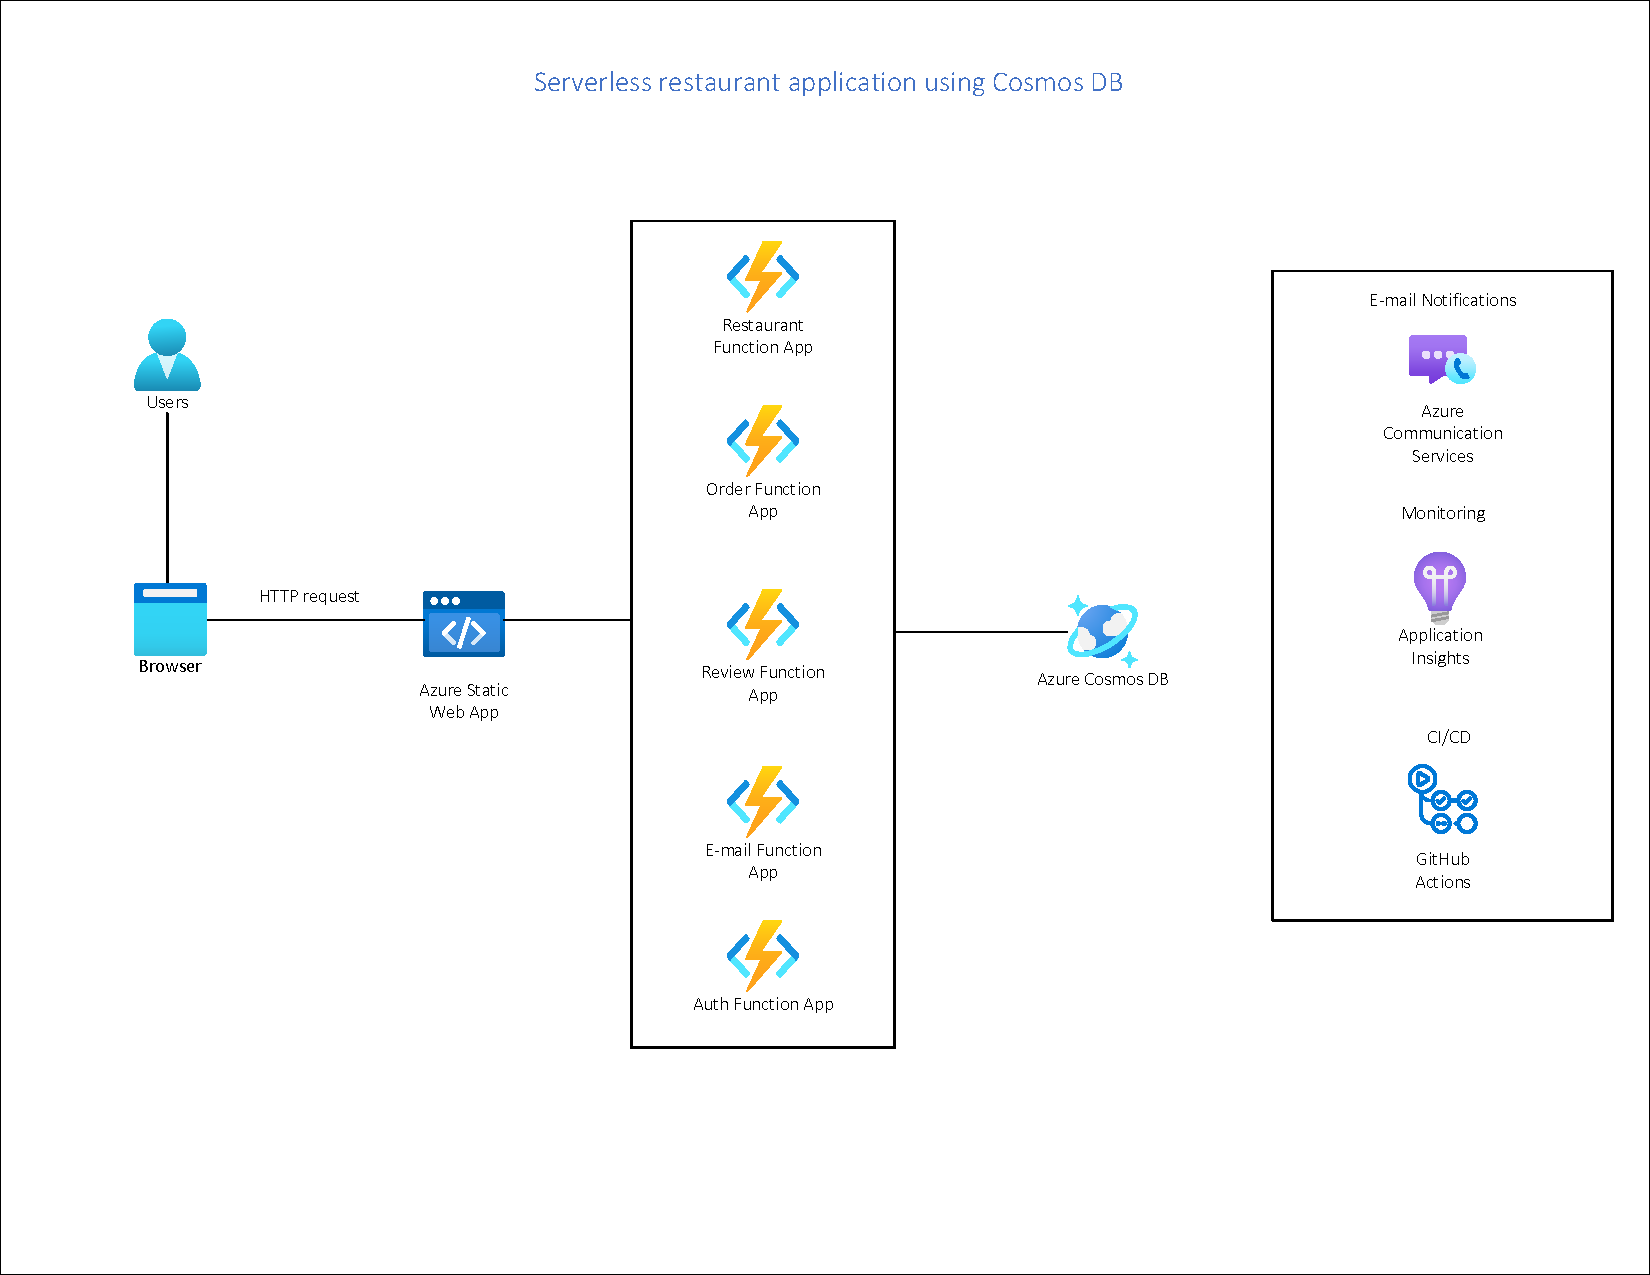
\includegraphics[width=150mm, keepaspectratio]{figures/AppArch}
	\caption{Restaurant application architecture diagram} 
	\label{fig:AppArch}
\end{figure}

%----------------------------------------------------------------------------
\subsection{Workflow}
%----------------------------------------------------------------------------

The architecture gets its input data from the user, who will send HTTP requests to an Azure Static Web App via the browser. The requests will trigger the underlying Function Apps and save or read the application data from Cosmos DB, which will be the architecture's main data service solution. I would like to use Azure Communication Services for e-mail notifications. Application Insights will provide debugging options on Azure. Finally, the app will be integrated with GitHub Actions to build and publish it to Azure.

%----------------------------------------------------------------------------
\subsection{Components}
%----------------------------------------------------------------------------

The components of my thought-out architecture are the following:

\begin{itemize}
	\item \textbf{Azure Static Web Apps} \emph{"is a service that automatically builds and deploys full stack web apps to Azure from a code repository."} It can interact with GitHub, so when a certain action is executed e.g.\ commit, the app builds and gets deployed automatically.\cite{StaticWebApps}
	
	\item \textbf{Azure Function Apps} is a FaaS platform to deploy compute-on-demand code without managing any underlying systems. \cite{ArchExample1}
	
	\item \textbf{Azure Cosmos DB} is a fully managed NoSQL database with nearly limitless scale. \cite{ArchExample1}
	
	\item \textbf{Azure Application Insights} is the native Application Perfirmance Management service in Azure which can be easily integrated with Web Apps and Azure Functions. \cite{ArchExample1}
	
	\item \textbf{Azure Communication Services} are cloud-based services which allow the developer to easily integrate different communication formats into his application such as e-mail, SMS or video. \cite{CommunicationServices}
	
	\item \textbf{GitHub Actions} According to GitHub, \emph{"GitHub Actions is a continuous integration and continuous delivery (CI/CD) platform that allows you to automate your build, test, and deployment pipeline. You can create workflows that build and test every pull request to your repository, or deploy merged pull requests to production."} \cite{GitHubActions}
	
\end{itemize}






%----------------------------------------------------------------------------
\chapter{Single Page Application implementation}\label{Ch3}
%----------------------------------------------------------------------------
 
 In this chapter I will discuss how the user flows we specified in Chapter \ref{Ch1} got implemented. I decided to work with Angular, the frontend framework that I have the most experience with and whose usage with Azure is well documented. My technique was to first create the user interface with mock data and then write the related services, so this is why I talk about this first here as well. 
 
%----------------------------------------------------------------------------
\section{User flow implementations}
%----------------------------------------------------------------------------
 
%----------------------------------------------------------------------------
\subsection{Anonymous User user flow}
%----------------------------------------------------------------------------

Previously, in Chapter \ref{AnonUserflow} we declared that users who first open the website should see a list of restaurants with some basic details (see Figure \figref{UIsAnon}) and be able to log in. So the first task was to decide what kind of data should be stored about the restaurants and how to display them in a user-friendly manner. These were implemented in the following files:

Components:
\begin{itemize}
	\item \verb+restaurants-list+: Gets the list of restaurants by calling restaurant service's function \verb+getRestaurants()+ and displays them. The items are clickable, therefore the user can navigate through them to the accompanying details page (see image at Appendix \figref{UI_1}).
	
	\item \verb+restaurant-details+: Gets the chosen restaurant by its id by calling the restaurant service's \verb+getRestaurantById(id)+ function and displays the restaurant details and its menu. The user can choose to order from the restaurant by clicking \textsc{order here} (see image at Appendix \figref{UI_2}). If the user is not logged in, he will be redirected to the login page and routed back to the order page after login.
	
	\item \verb+login+: The login page can be accessed by clicking the \textsc{order here} button at a restaurant's details page or by clicking \textsc{login} at the navbar, which is displayed on every page. This is a custom login page to the application, if the user does not have an account yet, he can choose to register either as guest or as restaurant (see image at Appendix \figref{UI_8}).
\end{itemize}
Models:
\begin{itemize}
	\item \verb+restaurant.type.ts+: Contains the \verb+Restaurant+ interface and other type declarations it uses e.g.\ \verb+MenuItems, Style+ enum.
	\item \verb+guest.type.ts+: The \verb+Guest+ interface is declared here, which is the interpretation of any logged in user. Guests and restaurants are distinguished by the \verb+restaurant+ attribute, which contains the restaurant id, if the user is a restaurant, otherwise it contains just an empty string.
\end{itemize}
Services:
\begin{itemize}
	\item \verb+restaurant.service.ts+: This service collects its data from the restaurant microservice, which will be discussed later in Section \ref{RestaurantMicroservice}. I will only mention the two functions we previously touched on:
	\begin{itemize}
		\item\verb+getRestaurants()+: The function calls the microservice with a get request and passes the result to the caller as an \verb+Observable+ object.
		\item\verb+getRestaurantById(id)+: This function acts the same way, except the request returns a single restaurant object instead of a list.
	\end{itemize}	
	\item \verb+auth.service.ts+: This service handles user login and logout and manages registrations. 
\end{itemize}

%----------------------------------------------------------------------------
\subsection{Guest user flow}
%----------------------------------------------------------------------------

Let's remember the requirements we set for the guest user flow (see Figure \figref{UIsGuest}). Here I mainly tried to accomplish two things: display a part of the restaurant data that is relevant for the ordering process and collect the guest's order details and send them to the database for further use. The main logic can be found in the following files:

Components:
\begin{itemize}	
	\item \verb+new-guest+: This is a very basic registration form, it collects the user's email, password and display name.
	
	
	\item \verb+registration-confirmation+: After filling the registration form, the user is prompted to add a confirmation code, which is sent to the provided e-mail address. While it is not filled successfully, the new user will not be registered. See image at \figref{UI_7.1}, \figref{UI_8.2} and \figref{UI_8.3}
	
	\item \verb+table-reservation+: This is the component where the order begins, the guest can decide to order takeaway and provide information about when he will arrive. If the order is eaten on-site, the user can reserve one or more tables for a given time interval on a tile map (see image at Appendix \figref{UI_4}). At the table selection map the tables are clickable and green-coloured if they are free at the order time, otherwise they are grey and non-clickable. They can also be chosen or removed at the side list. If the guest types in the required data, he can navigate to the menu or back to the details page. 
	\item \verb+menu+: The component lists the current restaurant's menu items, displays basic data about them and allows the guest to select the wished amount of dishes. The user can navigate to the cart component. See image at Appendix \figref{UI_5}
	\item \verb+cart+: The cart component summarises and displays all of the collected order data for the guest to revise it (see image at Appendix \figref{UI_3}). Changes in the amount of the dishes still can be made here. If the user removes all the dishes, he will be directed back to the menu page. The user can navigate back to order more or accept and proceed to payment. In this case the component calls the cart service's \verb+saveOrder()+ function to send the order data to the corresponding services.
	\item \verb+payment+: The payment component displays a confirmatory text about a hypothetic successful payment, the actual money transfer is not implemented. If the user navigates here, two e-mails going to be sent to his inbox via the email service with the payment and order details (see image at Appendix \figref{UI_7}).
	\item \verb+feedback-form+: After successfully submitting an order, the guest has the option to give feedback about the restaurant. The form asks the guest to score the restaurant on a scale from one to five, write a review and share his satisfaction with further aspects of the restaurant (see image at Appendix \figref{UI_14}). This review will be saved and affect the restaurant's rating and the review text will appear on the restaurant's details page. In a real life event this user feedback should be collected only after the expiration of the order's date, but for the sake of understanding I made it accessible here.
\end{itemize}
Models:
\begin{itemize}
	\item \verb+restaurant.type.ts+: See above.
	\item \verb+email.type.ts+: Contains three email interfaces, \verb+InvoiceEmail+, \verb+OrderEmail+. These are the collections of data that should be sent to the guest after order. 
	\item \verb+feedback.type.ts+: The interface that describes the guest's review.
\end{itemize}
Services:
\begin{itemize}
	\item \verb+restaurant.service.ts+: See above.
	\item \verb+cart.service.ts+: All of the order's collected data is handled by the cart service. When a user finishes the order process with payment, the cart service passes the order to the order service.
	\item \verb+email.service.ts+: This service communicates with the email microservice (discussed later at Section \ref{EmailMicroservice}). Separately collects and sends the order and payment data that will be displayed in the e-mails.
	\item \verb+review.service.ts+: Sends user reviews to the review microservice (see at Section \ref{ReviewMicroservice}).
	\item \verb+order.service.ts+: This service communicates with order microservice (see at Section \ref{OrderMicroservice}). It consists of the following functions:
	\begin{itemize}
		\item\verb+addOrder(order)+ function posts the guest's order to the microservice.
		\item\verb+getOrders(rId)+ (See at Restaurant user flow \ref{RestaurantSPA}).
		\item\verb+getOrdersToday(rId, date)+ (See at Restaurant user flow  \ref{RestaurantSPA}).
	\end{itemize}
\end{itemize}

%----------------------------------------------------------------------------
\subsection{Restaurant user flow}\label{RestaurantSPA}
%----------------------------------------------------------------------------
 
 The restaurant user flow should meet the requirements discussed in Section \ref{RestaurantUserflow} (also see Figure \figref{UIsRestaurant}). The following files contain the main logic of the user flow:
 
Components:
\begin{itemize}	
	\item \verb+edit-details+: This is the first component of the restaurant registration process and can be reached by clicking \textsc{new restaurant} on the login page.  It is a form where the new restaurant's basic details can be added. See image here: \figref{UI_9}
	\item \verb+edit-menu+:	The new restaurant user can add and remove menu items and save them or decide to make these settings later (see image at Appendix \figref{UI_10}). Empty dishes won't be saved.
	\item \verb+reservation-map+: This is the component where the user can edit a map of the restaurant's tables' layout. The map can have a name (in case later a restaurant could have more than one) and a photo can be uploaded of the room that the map portrays. The tile map itself can only be square shaped and the resolution can be between 5x5 and 17x17 (only odd numbers). Each tile displays empty floor by default and by clicking them the image changes to a table or other item whose location could affect a guest's table choice e.g.\ windows, food bar, toilets. If the tile displays a table then a seat number setting option appears on the right side of the map (see image at Appendix \figref{UI_11}). The user can choose to set it up later. By saving the map the new restaurant account is created and the user is directed to the login page. 
	\item \verb+dashboard+: When a user logs in to a restaurant account the dashboard component shows up. It contains the following:
	\begin{itemize}
		\item The restaurant's basic data and links to modifications.
		\item New orders shortlist with the three most recent order. By clicking \textsc{see all} the whole list can be viewed at a separate page.
		\item The orders for that day (if there is any).
		\item The reviews the guests wrote about the restaurant in the feedback form. The restaurant can write a reply if it haven't done so yet. This will appear on the restaurant's details page.
	\end{itemize}
The user can navigate back to the dashboard from anywhere by clicking the \textsc{Allegro} icon on the navbar.
	\item \verb+incoming-orders+: Displays the whole incoming orders list.
\end{itemize}
Models:
\begin{itemize}
	\item \verb+restaurant.type.ts+: See above.
	\item \verb+order.type.ts+: See above.
\end{itemize}
Services:
\begin{itemize}
	\item \verb+auth.service.ts+: See above.
	\item \verb+restaurant-admin.service.ts+: Handles the modifications that are made on a restaurant. Its most important function is \verb+addRestaurant(restaurant)+, which posts a new restaurant's JSON to the restaurant microservice.
	\item \verb+order.service.ts+: Two of order service's functions are relevant here.
	\begin{itemize}
		\item\verb+getOrders(rId)+: Fetches the given restaurant's orders' list from order microservice.
		\item\verb+getOrdersToday(rId, date)+: Gets the restaurant's orders from order microservice, whose booking day equals the day given in the parameter.
	\end{itemize}
	\item \verb+review.service.ts+: Its \verb+addAnswer(review, rId)+ function appends the restaurant's reply to an existing guest review. 
\end{itemize}

%----------------------------------------------------------------------------
\section{Serverless components}
%----------------------------------------------------------------------------
%----------------------------------------------------------------------------
\subsection{Setting up Azure Static Web Apps}
%----------------------------------------------------------------------------
As we have seen it in the previous chapter, to accomplish a serverless frontend, we will publish our app to Azure Static Web Apps. As it has a pretty easy-to-follow tutorial, I won't go into the step-by-step details of how to deploy a web app. There are more ways to go about it, I started out with a GitHub repository and followed the tutorials about creating a new static web app with angular \cite{SWADeploy}, adding an API \cite{SWAAddAPI} and connecting it to a function app \cite{SWAAddFuncApp}. Accomplishing the tutorials will result in a publicly available app. (Mine is available here: \ref{StaticWebAppLink}.) These tutorials do not include the routing configuration of the application, which by default can cause the problem that after reloading a page, the app will return error 404. This can be solved by creating a \emph{staticwebapp.config.json} file in the root folder and adding a navigation fallback (see full solution here: \cite{SWAConfig}). An other thing to pay attention to is deploying the local modifications to the web app manually. It is not too complicated in VS Code, but it's even simpler, if we automate the process with GitHub Actions.
%----------------------------------------------------------------------------
\subsection{Continuous Deployment with GitHub Actions}
%---------------------------------------------------------------------------- 
I created a CI/CD workflow with GitHub Actions \cite{CI/CDGitHubActions}. This way every time I push the app to GitHub, it will try to automatically deploy it to Static Web Apps. This can be configured via an yml file placed in the project's \verb+.github+ folder. My finished yml file can be visited at \ref{GitHubActionsYml}.
%----------------------------------------------------------------------------
\chapter{Managing Cosmos DB with Azure Functions}\label{Ch4}
%----------------------------------------------------------------------------

The backend of my application consists of five microservices. I will explain the creation of a microservice, then I will get on to my exact solution.  
%----------------------------------------------------------------------------
\section{Creating a Microservice with Azure Functions}
%----------------------------------------------------------------------------
In this case by microservice we will mean an Azure Function App. 
These are the steps for creating a new Azure Functions microservice: \cite{VSCodeFunction}

\begin{enumerate}
	\item Open an empty folder in VS Code.
	\item Hit F1 and choose Azure Functions: Create new project...
	\item Choose \verb+C#+ with .NET 6.0 LTS.
	\item To create the first Azure Function in the project, choose a trigger type. In this example I chose HTTP Trigger.
	\item Give it a name and select a namespace. My function is called AddReview and the namespace will be Review. Set Anonymous access rights.
\end{enumerate}
	
Now we have an Azure project with a basic Azure Function generated. It can be tested by hitting F5 in the console. All of our functions will be listed with their routes included, but for now we only have one: http://localhost:7071/api/AddReview. When we call it, we get the following response: (See Figure \figref{res})

\begin{figure}[!ht]
	\centering
	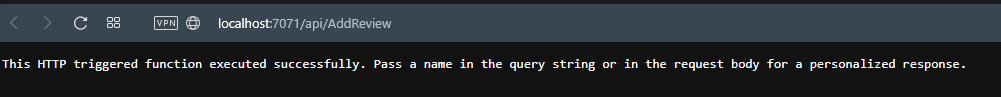
\includegraphics[width=150mm, keepaspectratio]{figures/4_response.png}
	\caption{Calling the function successfully.} 
	\label{fig:res}
\end{figure}

At this point we are free to make modifications to this function and then upload it to the cloud. But before publishing, we should create a Function App in Azure as this going to contain our functions. This can be achieved in VS Code as well. Hit F1 and choose \verb+Create Function App in Azure+ in the prompt. Sign in to Azure if needed and follow the instructions. I chose \verb+review-func-app+ as name, .NET 6 (non-isolated) runtime stack and a European location. When the resource is created, open again the Command Palette and choose \verb+Azure Functions: Deploy to Function App+ and select your freshly created function app. Click deploy and wait for the process to be finished, as this can take several minutes. At the bottom of the console output tab you should see the url to your published functions. They follow the pattern
\emph{https://your-func-app-name.azurewebsites.net/api/funcname}.

However calling these functions would end up giving an internal server error. Some modifications have to be made in the Azure Portal as well. These will be the following:
\begin{itemize}
	\item \textbf{Updating CORS}
	 In the search bar find your function app and on the sidebar, under API look for CORS. Here we type in all origins we would like to access this function app from, so the api will accept requests from these origins. I will add localhost with the default Angular port \emph{http://localhost:4200} and also the url of my published static app: \emph{https://ambitious-desert-085d2d503.1.azurestaticapps.net}. Save the modifications.
	 
	\item \textbf{Adding local settings to the portal}\label{LocalSettings}
	If the functions use (or will be using) Cosmos DB, then the connection string should be provided here and locally as well in \verb+local.settings.json+. Head to Configuration under Settings on the sidebar. Assuming that we already created a database, the connection string can be retrieved from multiple sources. In VS Code under Resources find your database, right click on it and choose Copy Connection String. In Azure Portal navigate to the Cosmos DB Account and on the sidebar under Settings select Keys and copy the Primary Connection String. Navigate back to the function app and add a New application setting, paste the Cosmos DB connection string under the value attribute and give it a name. Make sure to use this same name in your local settings and in your functions. Hit OK and Save the modifications.
\end{itemize}
  When all of this is finished, the function should work properly, in my case I could add a new review. (See Figure \figref{res_pub})

\begin{figure}[!ht]
	\centering
	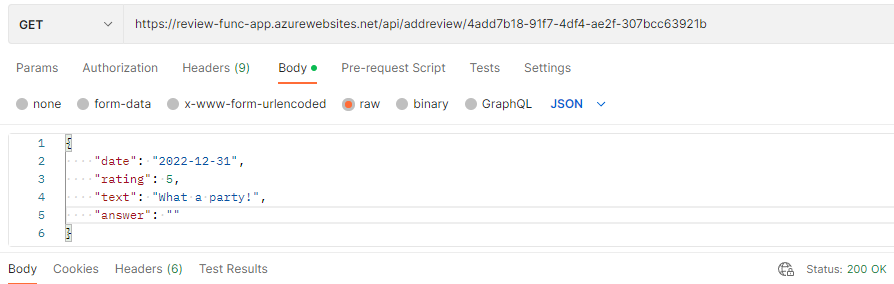
\includegraphics[width=150mm, keepaspectratio]{figures/7_published_response.png}
	\caption{Calling the function after publication.}
	\label{fig:res_pub}
\end{figure}

I did a small additional step, which is optional. I set up continuous deployment with GitHub Actions \cite{GitHubActionsForFunctions}, so every time I push the project to GitHub, it will be deployed automatically. This goes really quickly:

\begin{enumerate}
	\item Create an empty GitHub repository.
	\item Push the function app (its folder is initialized by default).
	\item Log in to Azure Portal at \url{https://portal.azure.com} and find the created function app.
	\item Navigate to Deployment Center on the sidebar.
	\item Select GitHub as source and authenticate with it.
	\item Select the function app's repository and a branch, whose content will be deployed.
	\item When you hit save, Azure will add a .yml file to the repository.
	\item Don't forget to pull this locally to avoid merge conflict.
	\item Modify the project and push it to GitHub.
\end{enumerate}

The changes should be deployed within a few minutes. (This process can be followed at the GitHub repository's Actions tab.)

%----------------------------------------------------------------------------
\section{Setting up a connection with Cosmos DB}
%----------------------------------------------------------------------------

Cosmos DB \cite{CosmosDBIntro} is a fully managed NoSQL database and compatible with multiple database APIs as Mongo DB, the native NoSQL API but also has relational database options. Fully managed in a sense that the user only has to create a resource in Azure and the database is ready to use, no further maintenance is needed (as previously mentioned in the Introduction). It is advertised with 99.999\% availability time and enterprise-grade security. Cosmos DB supports querying NoSQL API databases with SQL, in case of .NET Linq is also supported. 

Nearly all services will rely on some kind of data storage. In this case the application data is stored in Cosmos DB. The new database creation steps differ slightly based on the used framework and database API, but it has a solid documentation discussing all the options \cite{CosmosDBQuickstart}. If we would like to reach the created database from Azure Functions, we need an additional extension \ref{addCosmosDB} (see more detail at \cite{CosmosDBBinding}).

\lstset{ breaklines=true }
\begin{lstlisting}[frame=single,float=!ht, caption=Adding Cosmos DB to a Function App, label=addCosmosDB]
	dotnet add package Microsoft.Azure.WebJobs.Extensions.CosmosDB
\end{lstlisting}

My database structure is the following: the database file is called \emph{Restaurant} and includes three collections, \emph{RestaurantItems}, \emph{Orders} and \emph{Users}. These contain the single restaurant, order or user \emph{items} (read more about the Cosmos DB resource model here: \cite{CosmosDBResourceModel}). If we install the Azure Databases VS Code extension, we will be able to make changes and follow the database's state from the code editor's Azure tab by opening up the Resources dropdown (see image \figref{CosmosStructure}). 
\begin{figure}[!ht]
	\centering
	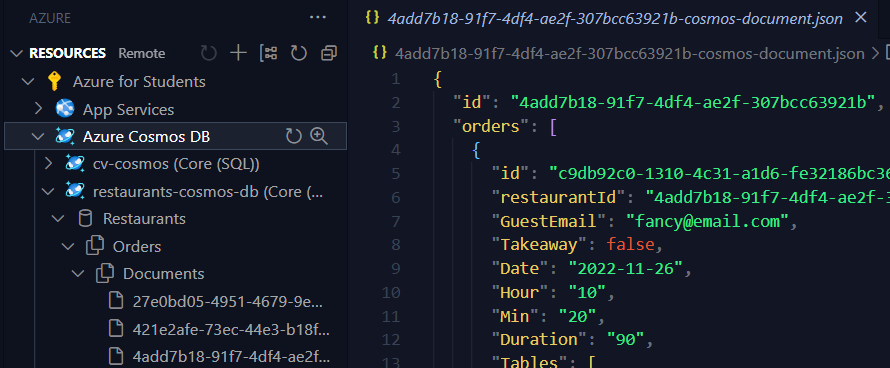
\includegraphics[width=150mm, keepaspectratio]{figures/DB/CosmosStructure.png}
	\caption{The database structure from VS Code} 
	\label{fig:CosmosStructure}
\end{figure}


%----------------------------------------------------------------------------
\section{Microservices}
%----------------------------------------------------------------------------
Now we proceed to discuss the app's services.
%----------------------------------------------------------------------------
\subsection{Auth Microservice}\label{RestaurantMicroservice}
%----------------------------------------------------------------------------

Auth Microservice is published at \ref{AuthMs}. It manages the user accounts, which are stored in the database's Users collection:

\begin{enumerate}
	\item \verb+AddUser+: Creates a new user document in the collection from the received JSON. 
	
	\item \verb+GetUserByEmail+: It performs a point read by the e-mail it gets in the route and returns the found user if any. E-mails are used as ids in this collection.
	
\end{enumerate}
Additional files:
\begin{enumerate}
	\item \verb+User.cs+: Describes the data structure of a user account.
\end{enumerate}

%----------------------------------------------------------------------------
\subsection{Restaurant Microservice}\label{RestaurantMicroservice}
%----------------------------------------------------------------------------
Restaurant Microservice is published at \ref{RestaurantMs}. It handles the RestaurantItems database collection and contains the following functions:

\begin{enumerate}
	\item \verb+GetAllRestaurants+: The function binds to the RestaurantItem collection and queries all of its items. Read more about Cosmos DB input binding here: \cite{CosmosDBInputBinding}
	\item \verb+GetRestaurantsWithFilter+: Works the same way as GetAllRestaurants, but parameters e.g.\ maxprice, rating can be sent to it. The function converts these to the wished format and filters the query results according to the given criteria.
	
	\item \verb+RestaurantById+: 
	It performs a point read by the id data it gets in the route and returns the result. Point reads are more cost effective than querying, so it is a good rule of thumb to use them whenever applicable \cite{CosmosDBCostOpt}. In my case the id and the partitionKey has the same value, but this is only because on creation I set up the container so. Overall, it is a good idea to set the id as partition key value, but note that it's not true to every database (find more on partitioning here: \cite{CosmosDBPartitioning}). 
	
	\item \verb+AddRestaurantOrchestration+: 
	This is a durable function orchestrator. Durable functions allow the developer to make chained or parallel function calls. I used the function chaining pattern here, which means that when the orchestrator is called, it will call the first function, waits to the evaluation then passes the result to the next function in the row (read more about the concept of durable functions here: \cite{DurableFunctions}).
	
	A durable function's entry point is a HttpStart function (by default gets the name myfunction\_HttpStart). It will call the orchestrator, wait for its execution and return the result. If we would like to pass JSON data to the functions called by the orchestrator, we should send it to the starter function, read the request data and pass it on as it is. The orchestrator can call functions in the same function app by their name or from anywhere else by their url. Read more about implementation details here: \cite{DurableFunctionsImplement}.
	
	How does this work in the context of our application? The function gets called, when a new restaurant is created by a user. It accomplishes three things: calls the \emph{AddRestaurantActivity}, which creates a new restaurant item document from the data that was sent in the request body. Generates a new id for it and adds it to the \emph{RestaurantItems} collection. This new id is returned back to the orchestrator and with it the \emph{addOrderRestaurant} function from the Order function app can be called, which creates an empty orders list for the restaurant. Finally, Auth function app's \emph{AddUser} function creates a new user with the restaurant's basic infos and generated id (see Figure \figref{durable}).	
	
	\begin{figure}[!ht]
		\centering
		
\includegraphics[width=150mm, keepaspectratio]{figures/Durable}
		\caption{Calls made by the orchestrator function} 
		\label{fig:durable}
	\end{figure}
	
\end{enumerate}

Additional files: 

\begin{enumerate}
	\item \verb+Restaurant.cs+: Contains the RestaurantItem class and some nested classes as Review or MenuItem. These describe the structure of the restaurantItem documents in Cosmos DB that's why the class contains the id and partitionKey attributes.
\end{enumerate}

%----------------------------------------------------------------------------
\subsection{Review Microservice}\label{ReviewMicroservice}
%----------------------------------------------------------------------------

Review Microservice is published at \ref{ReviewMs}. It handles the RestaurantItems collection's Reviews list. I decided to handle it separately as reviews are added to the document independently and seemed to form an independent unit logically. Although I didn't separate the database document, which at the time saved some coding but later turned out to be inconvenient. It would be better with a setup like in Order microservice even more so, because the Reviews list can grow boundlessly which can lead to problems \cite{NoSQLArrays}. The function app contains the following functions:

\begin{enumerate}
	\item \verb+AddReview+: This function saves user reviews of a restaurant. I used here the relatively new Partial Document Update feature, which allows us to modify an existing Cosmos DB document in one operation (see \cite{CosmosDBPartialDocumentUpdate}). This can be accessed via \ref{partialDoc}. 
	
	\lstset{ breaklines=true }
	\begin{lstlisting}[frame=single,float=!ht, caption=Adding Partial Document Update to a Function App, label=partialDoc]
		dotnet add package Microsoft.Azure.Cosmos
	\end{lstlisting}

	The AddReview function looks up the restaurantItem, whose id equals the id in the route. Then reads the review sent in the request body and creates a new review document, which will get the id with the current length of the restaurant's reviews list and then adds it to that exact index in the list. This solution is not flawless but I use it because partial document update can't manage array items by id, only by index. 	
	
	\emph{"If the target path is a valid array index, a new element will be inserted into the array at the specified index. It shifts existing elements to the right.
	If the index specified is equal to the length of the array, it will append an element to the array."  \cite{CosmosDBPartialDocumentUpdate}}
 	
	So if we would like to save ourselves from reading the list, finding the right item and get its index every time we have to update an item, then we should somehow store the index of each item. 
	
	This function class contains a few private attributes, I explain those later at the Startup.cs file's description.
	
	\item \verb+CalcRating+: Every time a new review is added by AddReview, it calls this function, which recalculates the connected restaurant's rating including the new review's rating. For this it reads the restaurant's reviews, sums up all reviews' rating and divides it by the review count, then updates the restaurant's rating attribute. Read more on output binding here: \cite{CosmosDBOutputBinding}
	I didn't use durable functions because it isn't a crucial task, if it runs successfully once in a while it will be enough.
	
	\item \verb+UpdateReview+: This function updates an already existing review. It is called, when a restaurant replies to a review. The function expects a review object in the request body and replaces it by its index (which we previously stored as the review's id). 
\end{enumerate}

Additional files: 

\begin{enumerate}
	\item \verb+Review.cs+: Contains the Review class and a RestaurantItem class, because the functions have to find the right restaurant item to read its reviews. This class only includes the attributes the review functions have to know about.
	
	\item \verb+Startup.cs+: Partial document update functions are accessible via the CosmosClient class, but unfortunately there is no support to bind it to an Azure Function. So we have to set it up in a separate Startup function, so the functions can retrieve them from here. Detailed steps about this can be found here: \cite{CosmosClient}
\end{enumerate}

%----------------------------------------------------------------------------
\subsection{Order Microservice}\label{OrderMicroservice}
%----------------------------------------------------------------------------

Order Microservice is published at \ref{OrderMs} and it handles the Orders collection. The collection's documents consist of a restaurant's id and a list of orders. 
I implemented the following functions:

\begin{enumerate}
	\item \verb+GetRestaurantOrders+: Reads and returns all orders from the document who's restaurant id equals the id in the route data. 
	
	\item \verb+GetOrdersToday+: Works the same way as GetRestaurantOrders, but filters the query results and returns only those, whose date equals the date route parameter's value.
	
	\item \verb+AddOrderRestaurant+: As I mentioned earlier, this function gets called by AddRestaurantOrchestration function, when a new restaurant was created. Gets the restaurant id as a route parameter and creates a new document with it. 
	
	\item \verb+AppendNewOrder+: It is called, when a user places a new order. The function creates an order object from the data it got in the request body. Then updates the orders list of the document whose id equals the order's restaurant id (with the help of partial document update).  

\end{enumerate}

Additional files: 

\begin{enumerate}
	\item \verb+Order.cs+: Containts the Order and OrderRestaurant classes. The latter consist of an id and an order list, the former gives the structure of an order.
	
	\item \verb+Startup.cs+: Same as in Review Microservice.
\end{enumerate}

%----------------------------------------------------------------------------
\subsection{Email Microservice}\label{EmailMicroservice}
%----------------------------------------------------------------------------

Email Microservice is published at \ref{EmailMs}. It sends out e-mails through the new Azure Communication Services. For this, I had to create a Communication Service resource \cite{CommunicationResource} and had to connect a domain to the resource \cite{ConnectEmailDomain}. I used an Azure domain, but a custom one can be set up as well. After installing the Azure Communication Services Email client library for .NET package (with the command \ref{addEmail}), we are ready to send e-mails \cite{SendEmail}. Note that this will only work locally. After publishing the function app, the connection string should be set in the Azure Portal too (the same way as the Cosmos DB connection string, we discussed it earlier here: \ref{LocalSettings}). 

\lstset{ breaklines=true }
\begin{lstlisting}[frame=single,float=!ht, caption=Adding the e-mail package to a Function App, label=addEmail]
	dotnet add package Azure.Communication.Email --prerelease 
\end{lstlisting}

 I created the following HTTP trigger functions:

\begin{enumerate}
	\item \verb+SendInvoiceEmail+: The function expects the e-mail data in the request body in the form of the \emph{EmailInvoice} class. Connects to the email client via the connection string, constructs the HTML content and sends the e-mail to the given e-mail address.
	
	\item \verb+SendOrderDetailsEmail+: Operates similarly to the previous function, but uses the EmailOrder class and the e-mail content differs.
	
	\item \verb+SendRegConfirmationEmail+: Used for confirming the e-mail address of a new guest. Sends the received code to the e-mail address.
\end{enumerate}

Additional files: 

\begin{enumerate}
	\item \verb+EmailData.cs+ file contains three classes, \emph{EmailOrder}, \emph{EmailInvoice} and \emph{EmailRegConfirmation}. They represent the collections of data sent in the corresponding e-mail type.
\end{enumerate}
%----------------------------------------------------------------------------
\chapter{Challenges and possible extensions}\label{Ch5}
%----------------------------------------------------------------------------

This is the application I could accomplish in the given time frame. Obviously it's not the best or most ideal solution to this problem. I will list a few things I would do differently next time or should be improved.

\begin{itemize}
	\item The user login would not be an acceptable solution in a real life environment. It is always a good idea to use an already existing and thoroughly tested service as Azure Active Directory. Instead of the hand written login, AD B2C should be introduced to this application.
	
	\item I should give more thought to the database structure and reshape it, if it turns out to be cumbersome to work with.
	
	\item Currently users can't delete anything from the database. Restaurants, orders and reviews should have a delete option.
\end{itemize}

Things that could be added to enhance the user experience:

\begin{itemize}
	\item At registration the restaurant users should get some feedback, that the registration was successful. Azure AD would solve this problem as well.
	
	\item Users could have a profile, which they could modify, maybe collect points or discounts if they use the app consistently.
	
	\item The feedback should be collected from the users after they actually went to the restaurant. This could be done via a timed email or if they would have a profile with the restaurants they can write a review for.
\end{itemize}
%----------------------------------------------------------------------------
\chapter{Evaluation}\label{sect:Comparison}\label{Ch6}
%----------------------------------------------------------------------------
%----------------------------------------------------------------------------
\section{Load testing results}
%----------------------------------------------------------------------------
%----------------------------------------------------------------------------
\subsection{Performance comparison}
%----------------------------------------------------------------------------
To examine the solution more in depth, I attempted to do a load test on the finished application. For this I used Azure Load Testing Preview \cite{LoadtestOverview}. Setting up a test was pretty straightforward. In order to run a quick test, I only had to create a testing resource and provide the test parameters such as the test url, count of generated users and test duration \cite{LoadtestQuickstart}. 

As I ran more intense tests against my application, I pretty fast reached a point where the test stopped because of the high number of failed requests. Digging into the results file I found that after a point nearly all requests got the \emph{429 - Too Many Requests} response. I'm not entirely sure why has this happened but my guess is that it was because I have a student Azure subscription and the amount of requests the static app can handle is limited. Researching the issue I have found that for some users Azure Static Web Apps caused similar problems.

Therefore, I decided to do a small test that fits into my resources and compare it to an SPA I created earlier and published to GitHub pages (\url{https://leventejuhos.github.io}). This is a one-page Angular app, it does not call any API. I tested both with 5 threads for 2 minutes.

I got the following test results for the two applications (see Figure \figref{swa} and Figure \figref{spa}):

\begin{figure}[!ht]
	\centering
	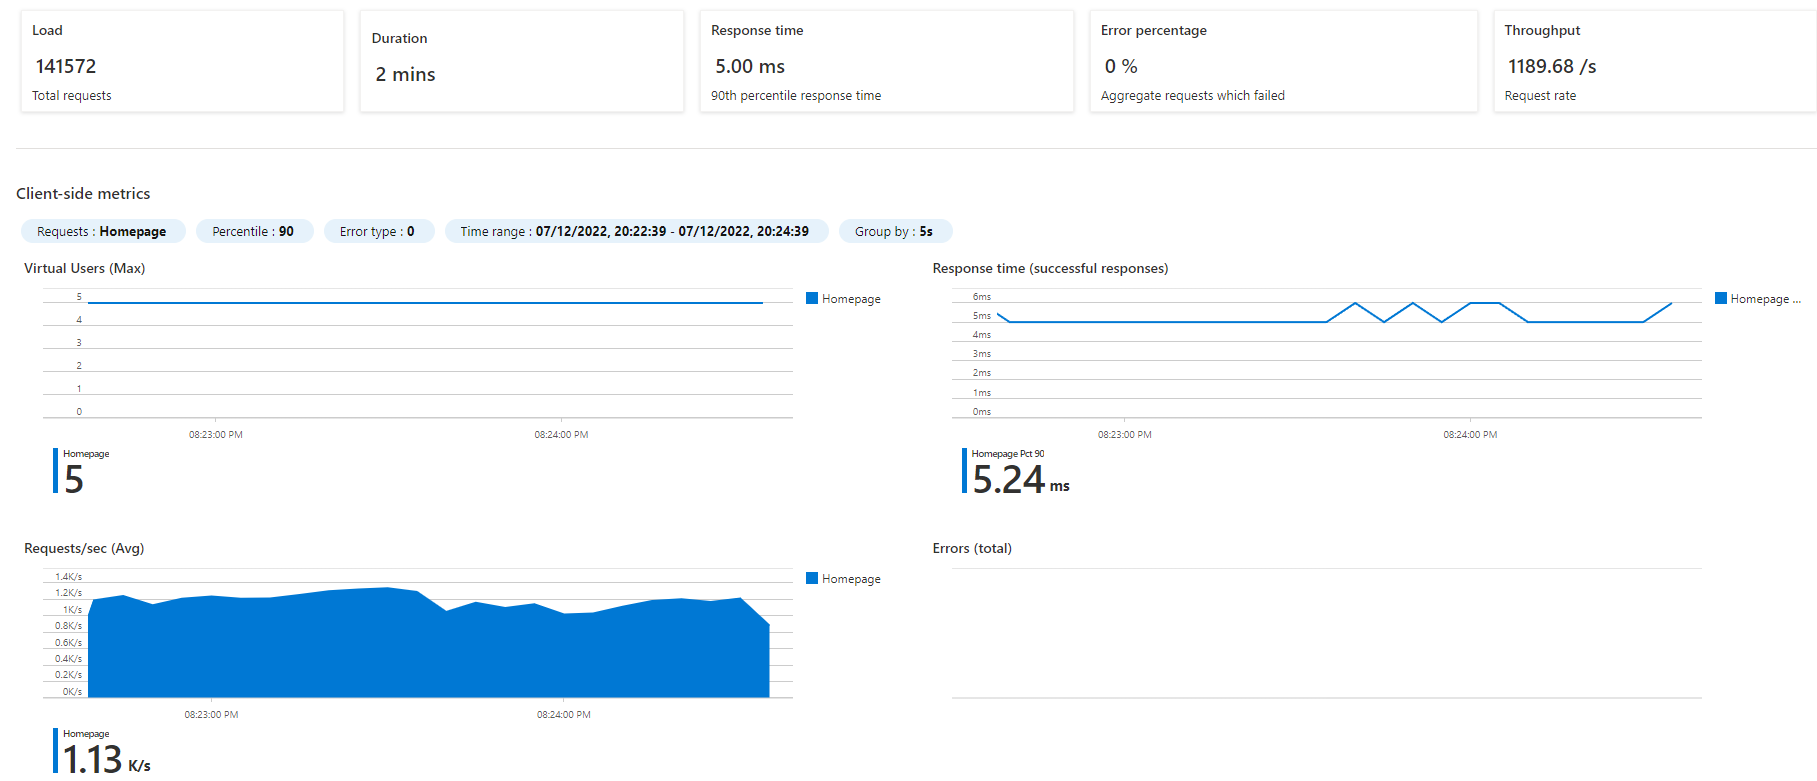
\includegraphics[width=150mm, keepaspectratio]{figures/loadtest/static_web_app.png}
	\caption{Static web app load testing results} 
	\label{fig:swa}
\end{figure}

\begin{figure}[!ht]
	\centering
	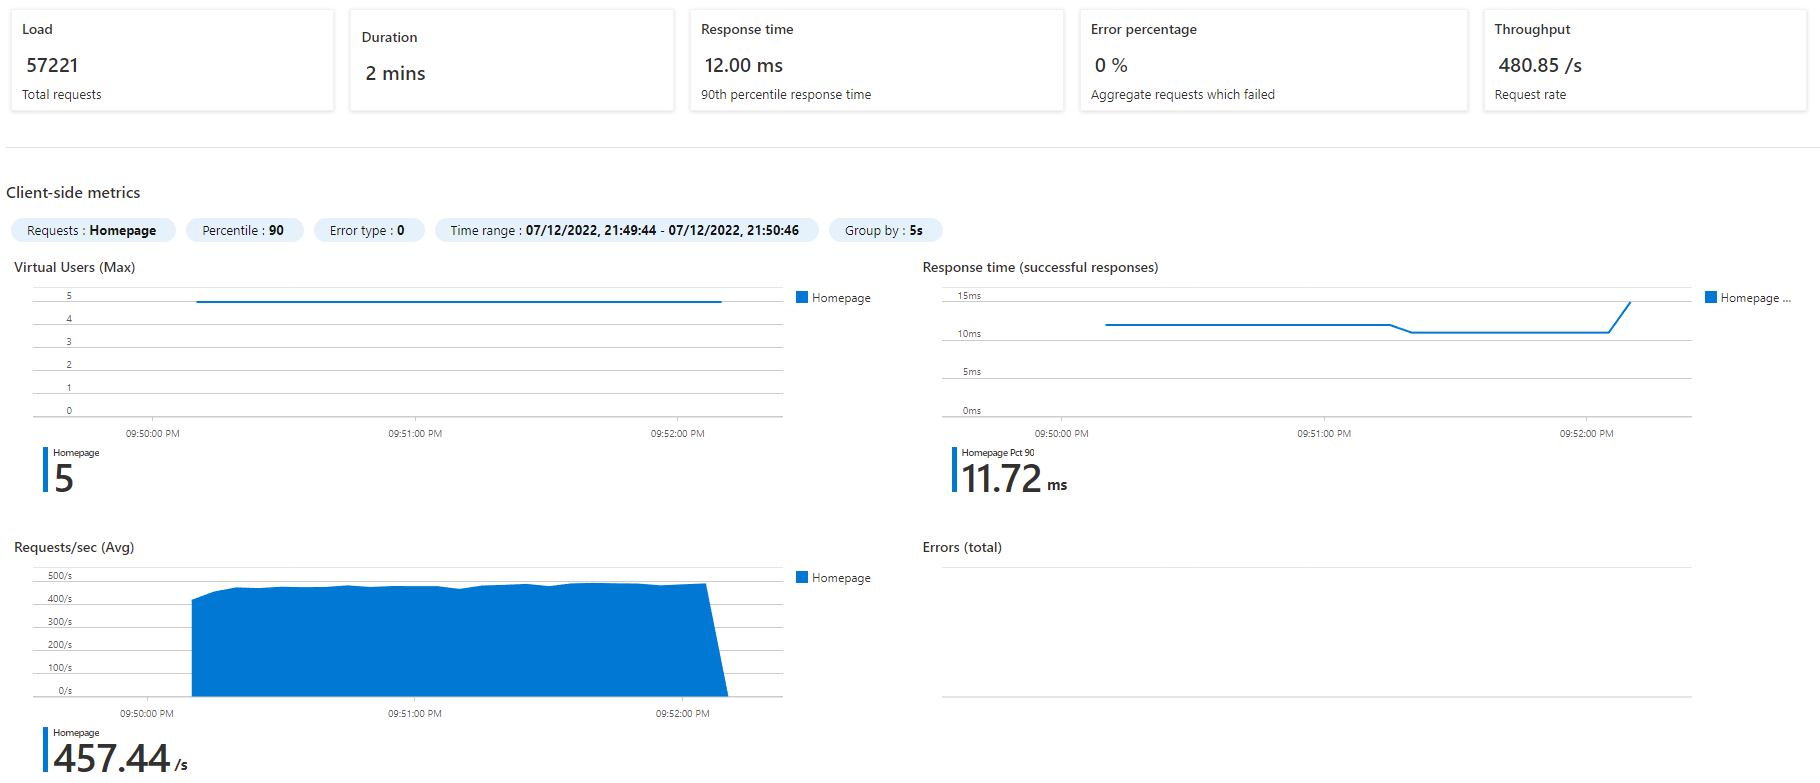
\includegraphics[width=150mm, keepaspectratio]{figures/loadtest/githubio-2.png}
	\caption{GitHub pages SPA load testing results} 
	\label{fig:spa}
\end{figure}

\begin{table}
	\begin{center}
		\begin{tabular}{||c c c c c c||} 
			\hline
			\makecell[c]{Name} & \makecell[c]{Thread count} & Duration  & \makecell[c]{Total requests} & \makecell[c]{Response time} & \makecell[c]{Requests/sec \\ (avg)}   \\ [0.5ex] 
			\hline\hline
			\makecell[c]{Azure \\ Static Web App} & 5 & 2 mins & 141572 & 5 ms & 1130/s \\
			\hline
			\makecell[c]{GitHub Pages \\ SPA} & 5 & 2 mins & 57221 & 12 ms & 457.44/s \\ [1ex] 
			\hline
		\end{tabular}
		\caption{App load testing results}
		\label{tab:AppLoadtest}
	\end{center}
\end{table}

When we compare the two (\tabref{AppLoadtest}) we see that despite the Azure web app calls a function and gets a list of about 50 items, it does better than the other app without any database request. The Azure app had a better response time, less than half of the SPA's and handled two and a half times the load volume of the SPA.

%----------------------------------------------------------------------------
\subsection{Service scalability}
%----------------------------------------------------------------------------

I gave another try to demonstrating the scalability of Azure by load testing one of the function apps. I set \url{https://restaurant-func-app-1.azurewebsites.net/api/getallrestaurants} function url as test url and run it for 2 minutes three times with different amount of virtual users.

\begin{table}
	\begin{center}
		\begin{tabular}{||c c c c c c||} 
			\hline
			\makecell[c]{Thread count} & Duration  & \makecell[c]{Total requests} & \makecell[c]{Response time} & \makecell[c]{Requests/sec \\ (avg)} & \makecell[c]{Error \\ percentage}  \\ [0.5ex] 
			\hline\hline
			10 & 2 mins & 14594 & 112 ms & 121.6/s & 0 \% \\
			\hline
			100 & 2 mins & 47244 & 364 ms & 377.46/s & 0 \% \\
			\hline
			250 & 2 mins & 60169 & 831 ms & 497.57/s & 0 \% \\ [1ex] 
			\hline
		\end{tabular}
		\caption{API load testing results}
		\label{tab:APILoadtest}
	\end{center}
\end{table}

This time none of the requests resulted in error. Comparing the results \tabref{APILoadtest} we notice that although the average response time did increase along with the demand, the number of served request/sec also increased significantly. If we take a look at the response time diagram (\figref{APIlt}), it looks like the system adapted quickly to the growing demand. The response time dropped steeply during the first few seconds and maintained this level for the rest of the test. 

\begin{figure}[!ht]
	\centering
	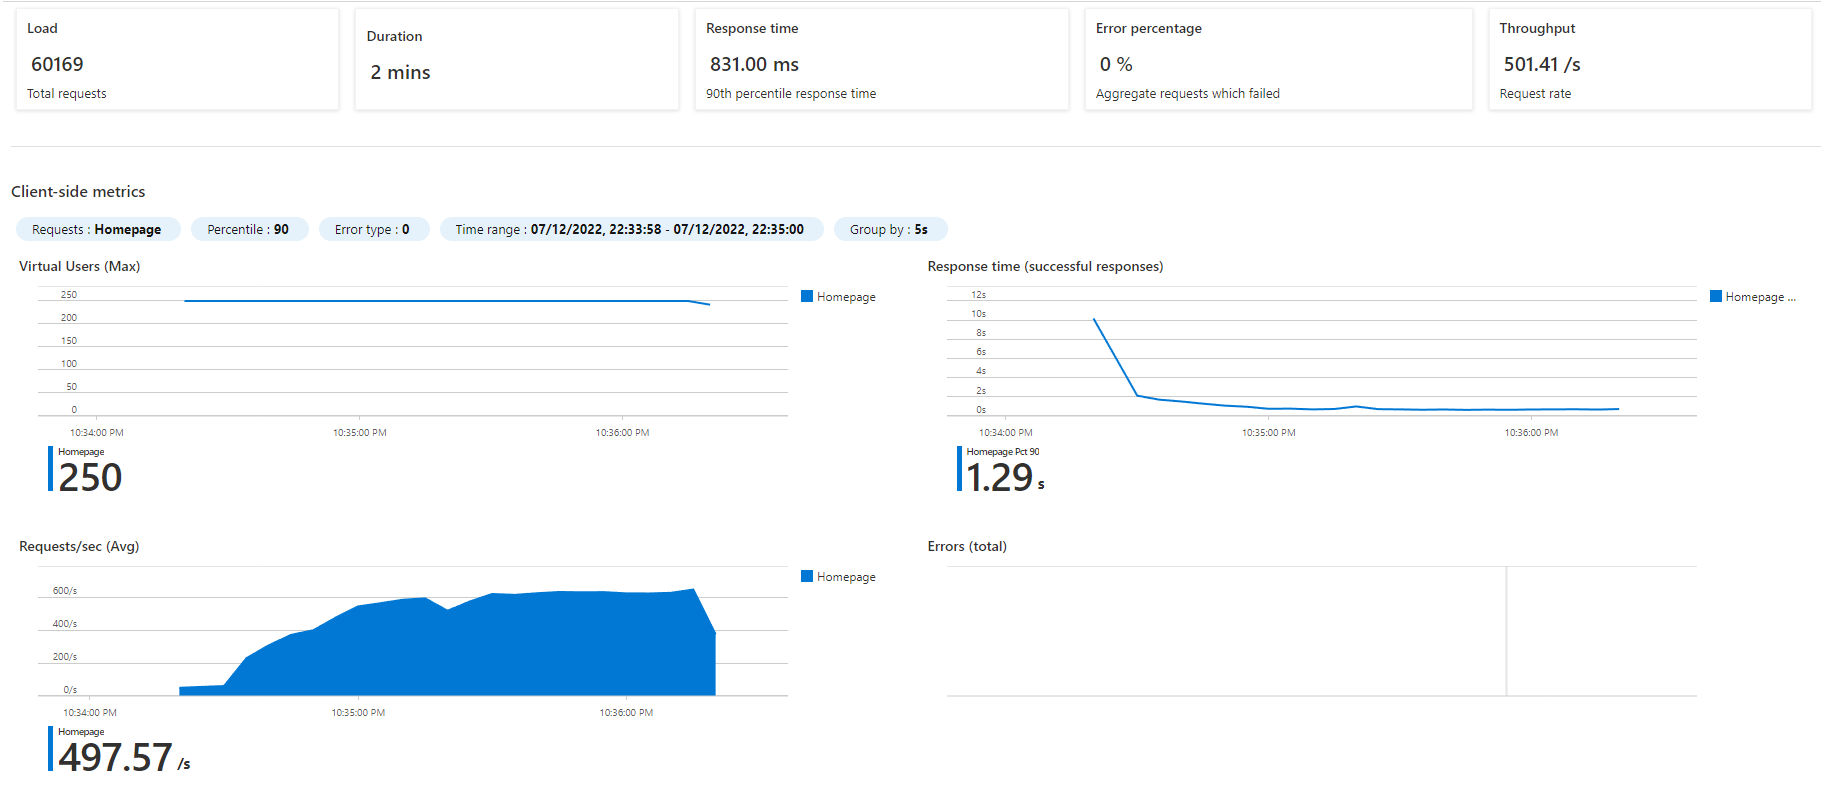
\includegraphics[width=150mm, keepaspectratio]{figures/loadtest/funcapp250-2.png}
	\caption{API load test with 250 threads} 
	\label{fig:APIlt}
\end{figure}

%----------------------------------------------------------------------------
\section{Solution complexity}
%----------------------------------------------------------------------------

After the load testing let's take a look at other aspects of the serverless solution. On the frontend part there wasn't much difference between a conventional and an Azure serverless solution nor should be. Azure Functions, on the contrary, worked substantially differently than the solutions I used before. They required some extra maintenance in the Azure portal, but I found the functions' code to be more distinct and easier to test. Actually, I was surprised by how little code had to be written in order to communicate with the database in comparison with a conventional app. Overall, in my experience the reading and finding out how some components can be reached from the functions took much of the time not the actual coding.

%----------------------------------------------------------------------------
\section{Code portability}
%----------------------------------------------------------------------------

One drawback of the serverless approach is that the user have to choose one provider and the migration between them is not obvious. The Angular SPA is easily moved and can be published on any chosen platform. I could publish this exact same code anywhere else than Azure Static Web Apps without further modifications. Unfortunately, we can't state the same about Azure Functions. Migrating a simple HTTP triggered function between cloud providers shouldn't be a huge hurdle. However, when Cosmos DB or other Azure specific components come into play then these have to be replaced by the other provider's solution, which will mean modifications in the function code as well. This is equally true to the data storage. As Azure is around for some time now there are solutions for moving data to other providers, but these will require extra steps from the developers' part (see an example here: \cite{MongoMoveData}).
%----------------------------------------------------------------------------
\chapter{Summary}\label{Ch7}
%----------------------------------------------------------------------------
Here I will summarize my impressions while working on this project.
%----------------------------------------------------------------------------
\section{Azure Serverless}
%----------------------------------------------------------------------------
Overall I had a pleasant experience with Microsoft Azure. One doesn't have to know everything to start. Azure is most of the time well documented. I worked with services that got published recently e.g.\ Communication Services for email sending or Partial Document Update for Cosmos DB. Most of the time I could use these by only reading the official documentation. On the rare occasion I needed a more specific solution, there were developers who already faced the same issue and came to some solution so I could figure out the missing parts by myself. The usage of the software was for the most part straightforward and there is a fairly reliable community.

One aspect what developers often complain of is the difficulty of debugging the server side. Granted, the error messages were some of the time non-existent. Occasionally waiting a little bit longer solved the problem and the function worked afterwards. When it did not help, testing the service locally and following the small leads I got did and the issues turned out to be discoverable and solvable. Later on when I collected a bit of experience I could guess what caused the bug. Note that mine was only a small example and in a huge system it's probably not that easy and not a good idea to rely on assumptions.
%----------------------------------------------------------------------------
\section{Microservices}
%----------------------------------------------------------------------------
Another thing I became a big fan of are microservices. At first it took some time to figure out their usage but then it turned out to be a handy tool. I did not get lost in the code base, which is a big plus especially in case of a big project. Testing and modifying the functions was straightforward, it wasn't a concern from which part of the API an error comes, because there were distinct collections of files that were not dependent on each other.
An additional benefit of this is that each microservice can have its own configuration, which reduces the number of installed packages to only those, which are used by that service's functions.

The price for this convenience is that it takes extra effort. Nonetheless, in my experience they save a lot more time than it takes to set up each of them, what went reasonably fast with Azure.

%----------------------------------------------------------------------------
\chapter*{Acknowledgements}\addcontentsline{toc}{chapter}{Acknowledgements}
%----------------------------------------------------------------------------

I would like to thank my advisor, Gábor Simon for the support and patience he provided so this thesis could be carried out.

%\listoffigures\addcontentsline{toc}{chapter}{Ábrák jegyzéke}
%\listoftables\addcontentsline{toc}{chapter}{Táblázatok jegyzéke}

\bibliography{mybib}
\addcontentsline{toc}{chapter}{Bibliography}
\bibliographystyle{plain}

%----------------------------------------------------------------------------
\appendix
%----------------------------------------------------------------------------
\chapter*{Appendices}\addcontentsline{toc}{chapter}{Appendices}
\setcounter{chapter}{1}  % a fofejezet-szamlalo az angol ABC 6. betuje (F) lesz
\setcounter{equation}{0} % a fofejezet-szamlalo az angol ABC 6. betuje (F) lesz
\numberwithin{equation}{section}
\numberwithin{figure}{section}
\numberwithin{lstlisting}{section}

%----------------------------------------------------------------------------
\section{Link collection}\label{links}
%----------------------------------------------------------------------------

GitHub Actions yml file:\newline \url{https://github.com/dormico/restaurant-reservation-system/blob/master/.github/workflows/azure-static-web-apps-ambitious-desert-085d2d503.yml}\label{GitHubActionsYml}

Static web app GitHub Repository:\newline \url{https://github.com/dormico/restaurant-reservation-system}\label{GitHubRepo}

Auth microservice GitHub Repository:\newline \url{https://github.com/dormico/restaurant-reservation-system-auth}\label{GitHubRepoAuth}

Email microservice GitHub Repository:\newline \url{https://github.com/dormico/restaurant-reservation-system-email}\label{GitHubRepoEmail}

Orders microservice GitHub Repository:\newline \url{https://github.com/dormico/restaurant-reservation-system-orders}\label{GitHubRepoOrder}

Restaurant microservice GitHub Repository:\newline \url{https://github.com/dormico/restaurant-reservation-system-restaurant}\label{GitHubRepoRestaurant}

Review microservice GitHub Repository:\newline \url{https://github.com/dormico/restaurant-reservation-system-review}\label{GitHubRepoReview}

Published Static Web App:\newline \url{https://ambitious-desert-085d2d503.1.azurestaticapps.net}\label{StaticWebAppLink}

Published Auth Microservice: \url{https://auth-func-app.azurewebsites.net/api/}\label{AuthMs}

Published E-mail Microservice: \url{https://email-func-app.azurewebsites.net/api/}\label{EmailMs}

Published Order Microservice: \url{https://orders-func-app.azurewebsites.net/api/}\label{OrderMs}

Published Restaurant Microservice: \url{https://restaurant-func-app-1/api/}\label{RestaurantMs}

Published Review Microservice: \url{https://review-func-app.azurewebsites.net/api/}\label{ReviewMs}

\newpage

%----------------------------------------------------------------------------
\section{Use Cases' List}\label{usecases}
%----------------------------------------------------------------------------

\textbf{Actors:} 
\begin{itemize}
	\item Anonymous User
	\item Guest
	\item Restaurant
\end{itemize}
\begin{table}[ht]
	\centering
	\caption{Use Cases} \label{tab:use-cases}
	\begin{tabular}{ | l | l |}
		\hline
		\textbf{Title} & \textbf{Listing restaurants} \\ \hline
		Actor & Anonymous user \\ \hline
		Trigger & Anonymous user opens the application \\ \hline
		Basic flow & Every restaurant gets listed \\
		\hline
		& \\
		\hline
		\textbf{Title} & \textbf{Arrange restaurants' list} \\ \hline
		Actor &  Anonymous user \\ \hline
		Basic flow & \makecell[l]{Anonymous user can arrange the restaurants based on various attributes \\ (e.g. price category, food type, opening hours, rating)} \\
		\hline
		& \\
		\hline
		\textbf{Title} & \textbf{Detailed information on a restaurant} \\ \hline
		Actor &  Anonymous user \\ \hline
		Preconditions &  Restaurants' list is available \\ \hline
		Trigger & Anonymous user clicks on a restaurant on the list \\ \hline
		Basic flow & \makecell[l]{Restaurant details are shown \\ (e.g. price category, type of food, menu, opening hours)} \\
		\hline
		& \\
		\hline
		\textbf{Title} & \textbf{View restaurant evaluations} \\ \hline
		Actor &  Anonymous user \\ \hline
		Preconditions &  User chose a restaurant \\ \hline
		Basic flow & \makecell[l]{ Restaurant evaluations and existing answers are shown publicly } \\
		\hline	
		& \\
		\hline
		\textbf{Title} & \textbf{Login} \\ \hline
		Actor &  Guest, Restaurant \\ \hline
		Preconditions &  The user has an account \\ \hline
		Basic flow & Guests and Restaurants can log in to the application \\ \hline
		Alternative flow & If the Guest or Restaurant doesn't have an account, he should create one \\
		\hline	
		& \\
		\hline
		\textbf{Title} & \textbf{Registration as Guest} \\ \hline
		Actor &  Anonymous user \\ \hline
		Basic flow & \makecell[l]{ Guests can register to the application by providing their \\ e-mail address and a password.} \\ 
		\hline		
	\end{tabular}
	\label{tab:TabularExample}	
\end{table}		
\begin{table}[ht]
	\centering
	\caption{Use Cases}
	\begin{tabular}{ | l | l |}	
		\hline
		\textbf{Title} & \textbf{Registration as Restaurant} \\ \hline
		Actor &  Anonymous user \\ \hline
		Basic flow & \makecell[l]{ Restaurants can register by providing the restaurant's name, \\ contact information (e-mail and phone number), location, menu with prices, \\ opening hours, whether they prepare food for takeaway or not and a password.} \\ 
		\hline
		& \\
		\hline
		\textbf{Title} & \textbf{Choosing time interval} \\ \hline
		Actor &  Guest \\ \hline
		Preconditions &  Guest is logged in, a restaurant is chosen \\ \hline
		Basic flow & Guest can choose reservation time. \\ 
		\hline
		& \\
		\hline
		\textbf{Title} & \textbf{Table reservation} \\ \hline
		Actor &  Guest \\ \hline
		Preconditions &  Guest is logged in, chose a restaurant and an arrival time \\ \hline
		Basic flow & The guest can reserve one or more table(s) \\ \hline
		Alternative flow & \makecell[l]{ The Guest doesn't reserve a table, but orders takeaway instead \\ (if the chosen restaurant
		allows).} \\
		\hline
		& \\
		\hline
		\textbf{Title} & \textbf{Ordering meal} \\ \hline
		Actor &  Guest \\ \hline
		Basic flow & Guests can order dishes from the menu and set the amount of them \\
		\hline
		& \\
		\hline
		\textbf{Title} & \textbf{Payment} \\ \hline
		Actor &  Guest \\ \hline
		Preconditions &  Guest is logged in, ordered meals \\ \hline
		Basic flow & The guest pays for the order \\ 
		\hline
		& \\
		\hline
		\textbf{Title} & \textbf{Guest receives confirmation e-mail} \\ \hline
		Actor &  Guest \\ \hline
		Trigger &  Guest payed for a meal \\ \hline
		Basic flow & Guest receives an e-mail about the details of the order \\ 
		\hline		
		& \\
		\hline
		\textbf{Title} & \textbf{Guest asked to evaluate service} \\ \hline
		Actor &  Guest \\ \hline
		Precondition &  Guest payed for a dish \\ \hline
		Basic flow & \makecell[l]{ The guest receives a link to a satisfaction questionnaire. \\ By clicking it he can give feedback on whether the restaurant and \\ the application met his expectations. (e.g. he got a table, the food was \\ served on time, overall impression and rating of the place) } \\ 
		\hline	
		& \\	
		\hline
		\textbf{Title} & \textbf{Restaurant receives order} \\ \hline
		Actor &  Restaurant \\ \hline
		Trigger &  Guest payed for a dish \\ \hline
		Basic flow & \makecell[l]{ If a guest orders something in the application, \\ the restaurant receives a notification with the order details \\ (e.g. time, number of persons, ordered meals) } \\ 
		\hline			
	\end{tabular}
\end{table}
\begin{table}[ht]
	\centering
	\caption{Use Cases}
	\begin{tabular}{ | l | l |}	
		\hline
		\textbf{Title} & \textbf{Restaurant lists existing orders} \\ \hline
		Actor &  Restaurant \\ \hline
		Precondition &  Restaurant has an account, and has existing orders \\ \hline
		Basic flow & \makecell[l]{ Restaurant can list existing orders and arrange them by various attributes \\ (e.g. time of the
		reservation, number of persons) } \\ 
		\hline	
		& \\
		\hline
		\textbf{Title} & \textbf{View order statistics} \\ \hline
		Actor &  Restaurant \\ \hline
		Precondition &  The restaurant has at least one order \\ \hline
		Basic flow & \makecell[l]{ Restaurant can watch statistics of orders (e.g. most liked dish, popular timeslots) } \\ 
		\hline
		& \\
		\hline
		\textbf{Title} & \textbf{Reply to evaluation} \\ \hline
		Actor &  Restaurant \\ \hline
		Precondition &  The restaurant has at least one evaluation \\ \hline
		Basic flow & \makecell[l]{ The restaurant can reply to evaluations. } \\ 
		\hline
	\end{tabular}
\end{table}

\newpage
%----------------------------------------------------------------------------
\section{User Interface examples}\label{UIex}
%----------------------------------------------------------------------------
\begin{figure}[ht]
	\centering
	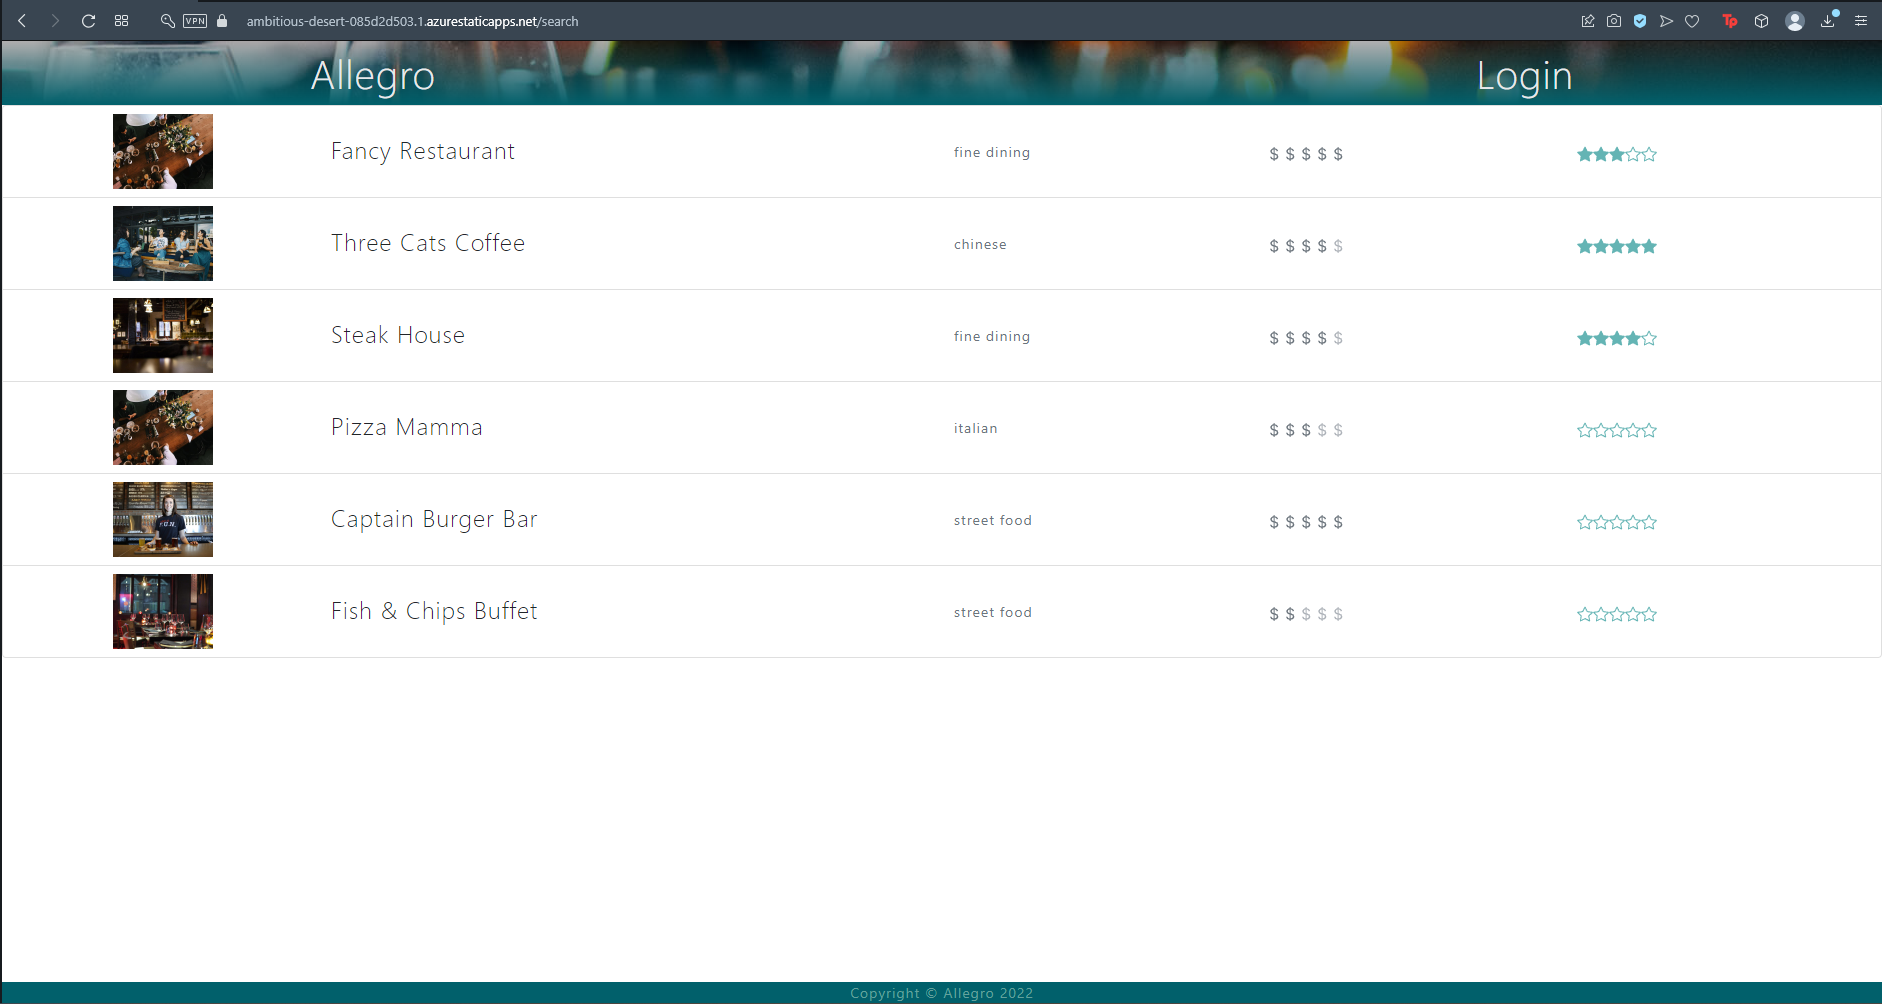
\includegraphics[width=150mm, keepaspectratio]{figures/UI/1_RestaurantList.png}
	\caption{Restaurant list component UI} 
	\label{fig:UI_1}
\end{figure}

\begin{figure}[ht]
	\centering
	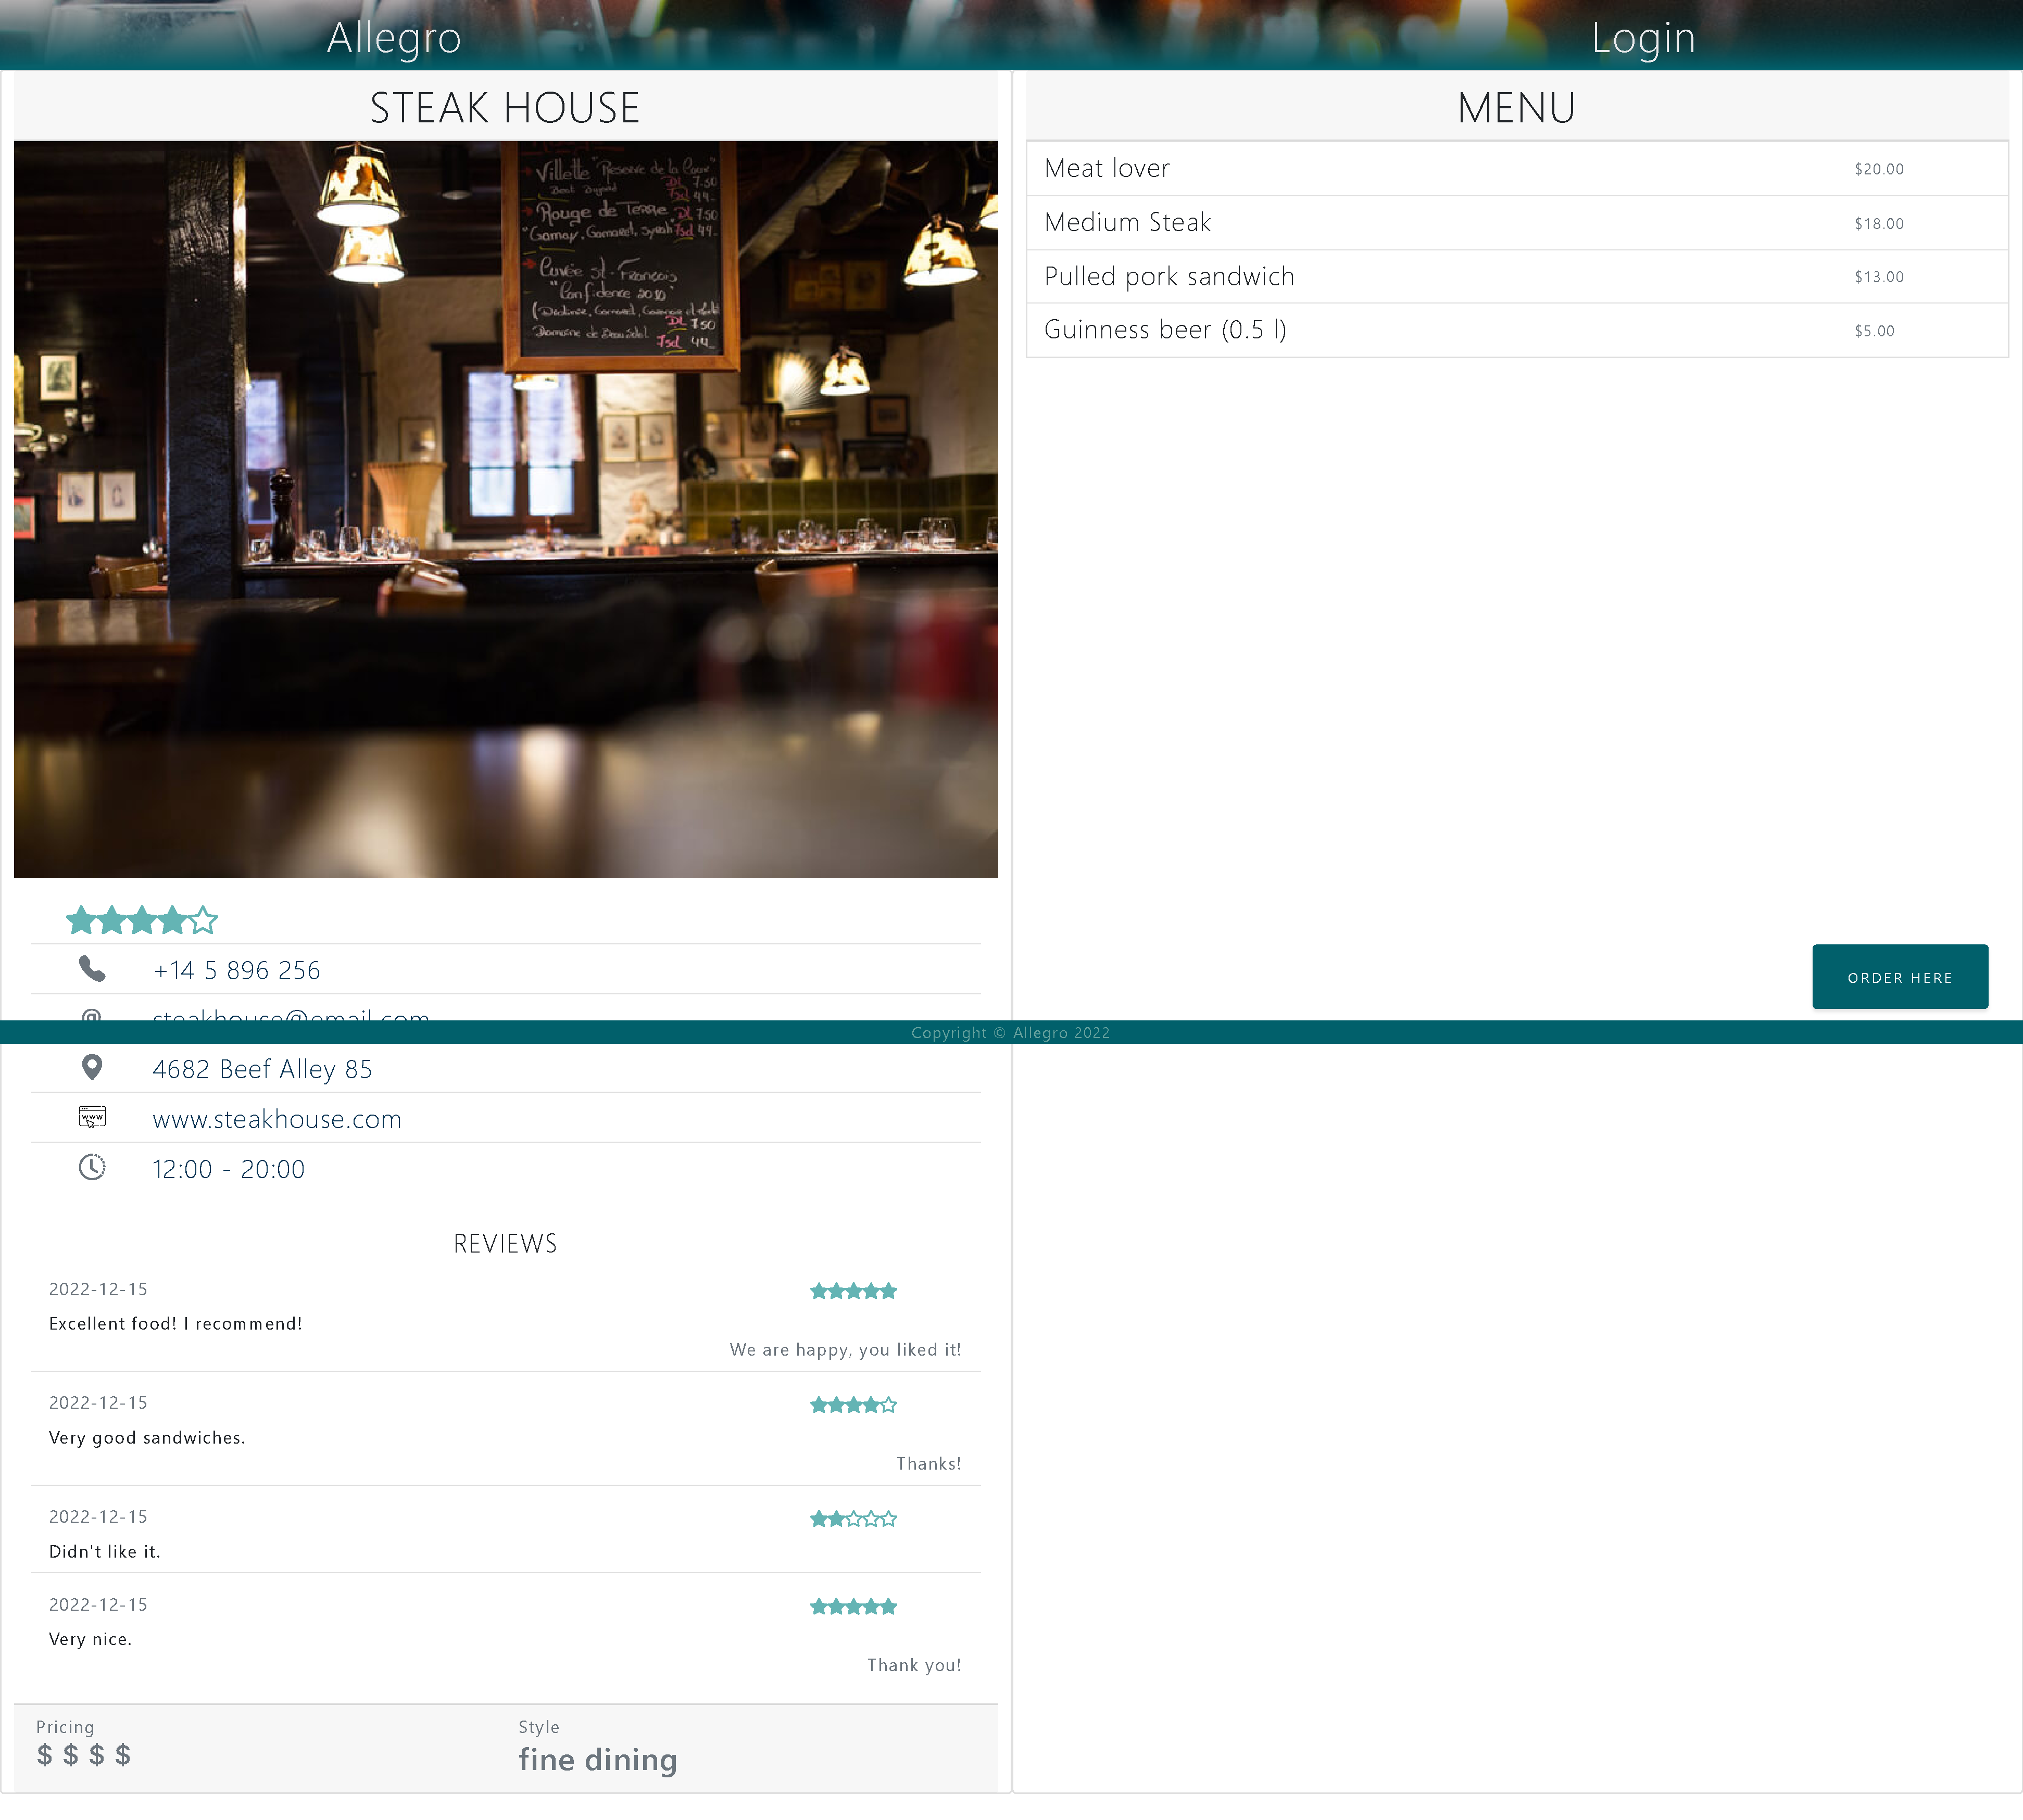
\includegraphics[width=150mm, keepaspectratio]{figures/UI/2_RestaurantDetails}
	\caption{Restaurant details component UI} 
	\label{fig:UI_2}
\end{figure}

\begin{figure}[ht]
	\centering
	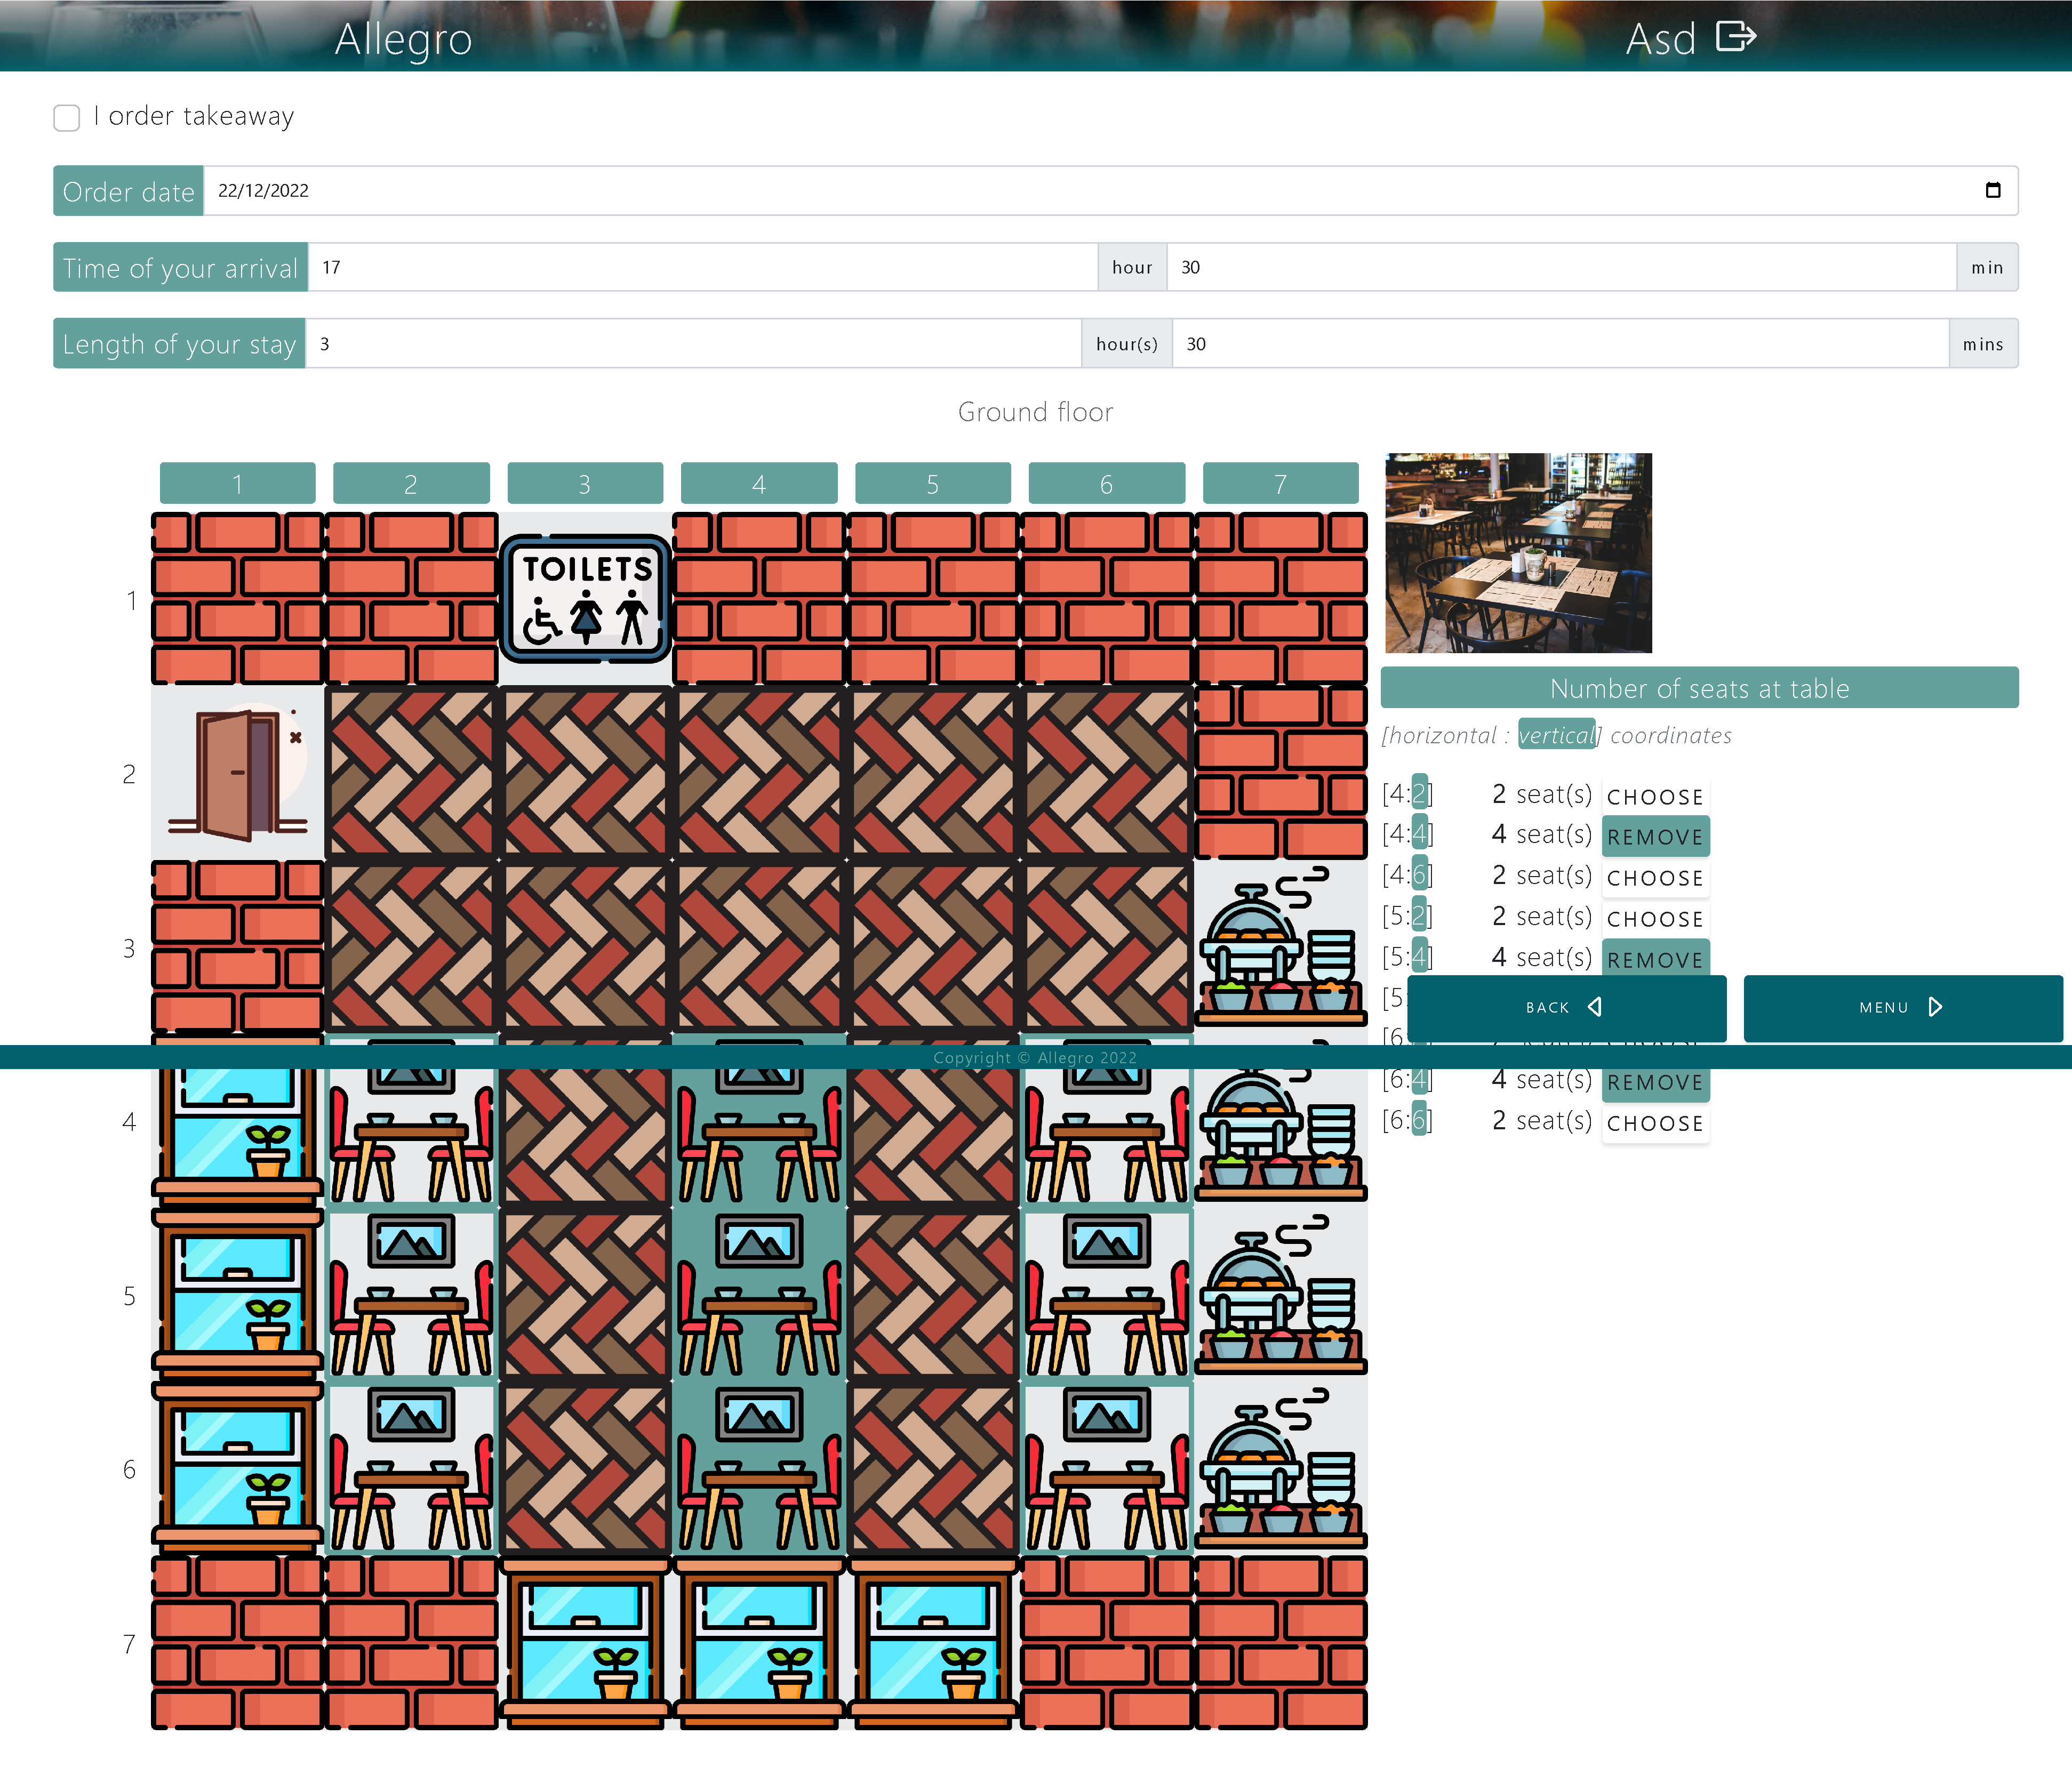
\includegraphics[width=150mm, keepaspectratio]{figures/UI/4_Reservation}
	\caption{Reservation component UI} 
	\label{fig:UI_4}
\end{figure}

\begin{figure}[ht]
	\centering
	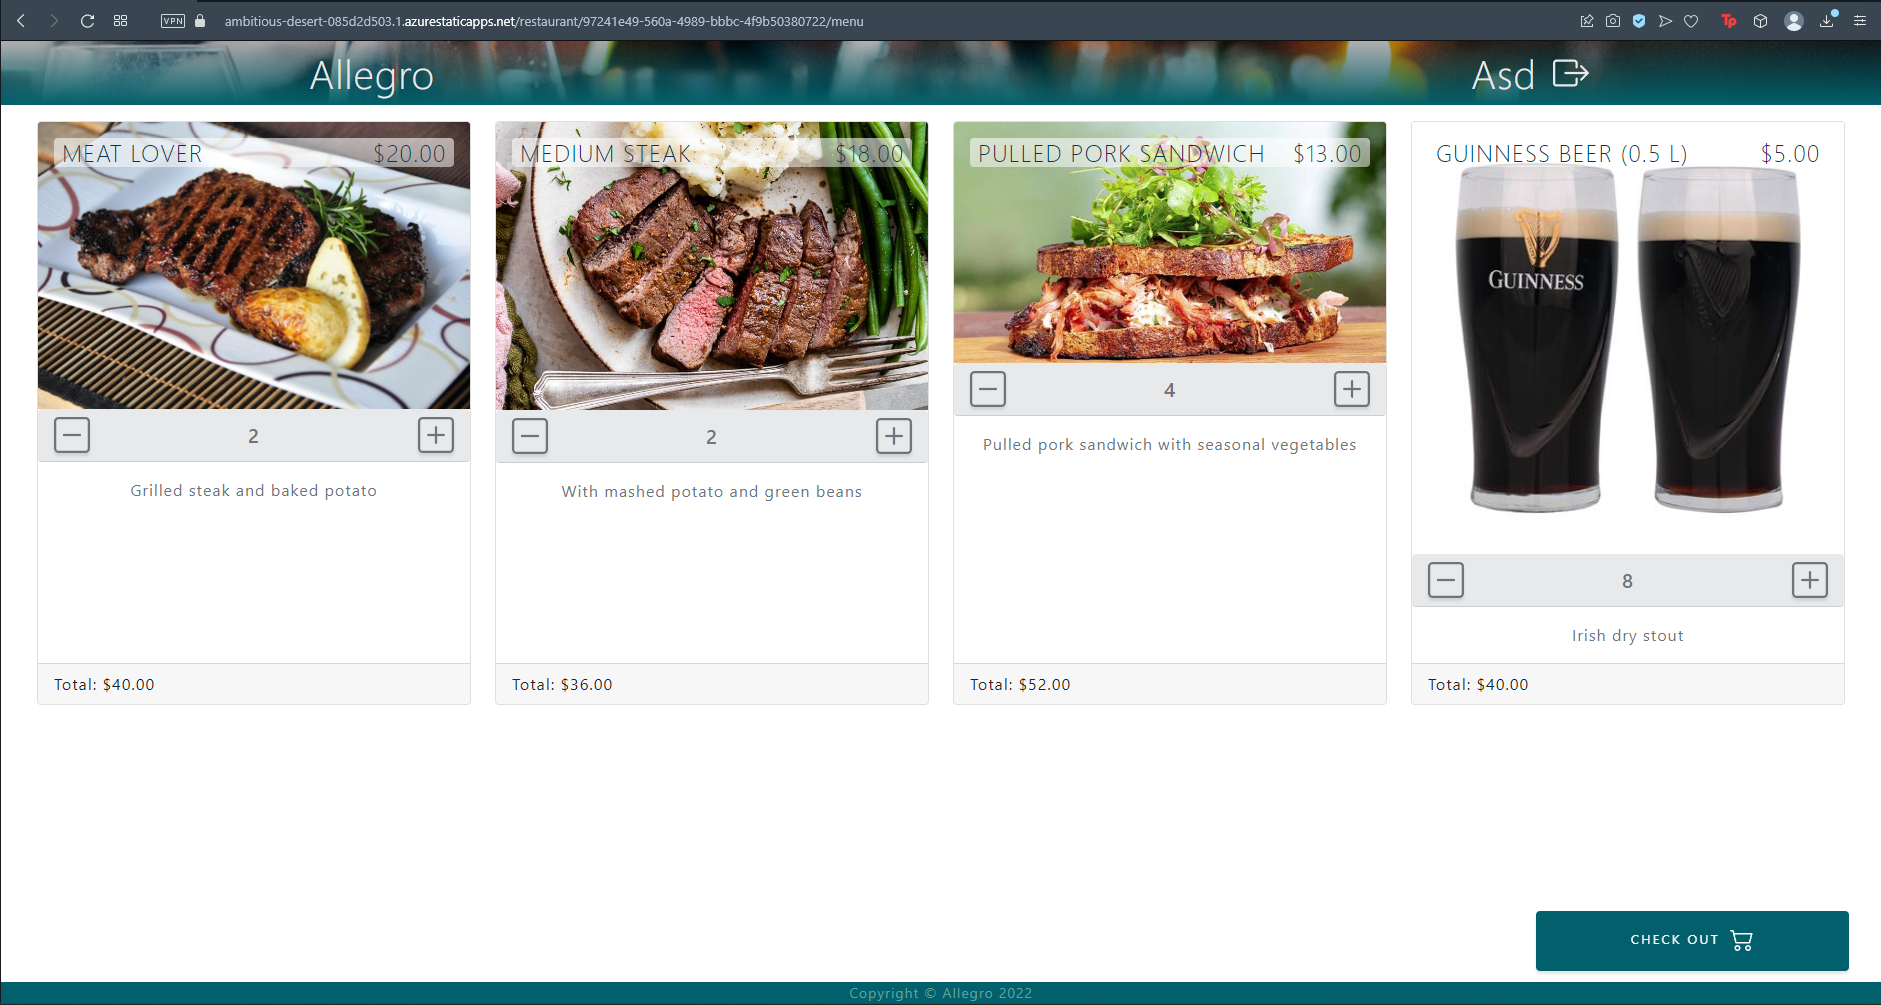
\includegraphics[width=150mm, keepaspectratio]{figures/UI/5_Order.png}
	\caption{Order component UI} 
	\label{fig:UI_5}
\end{figure}

\begin{figure}[ht]
\centering
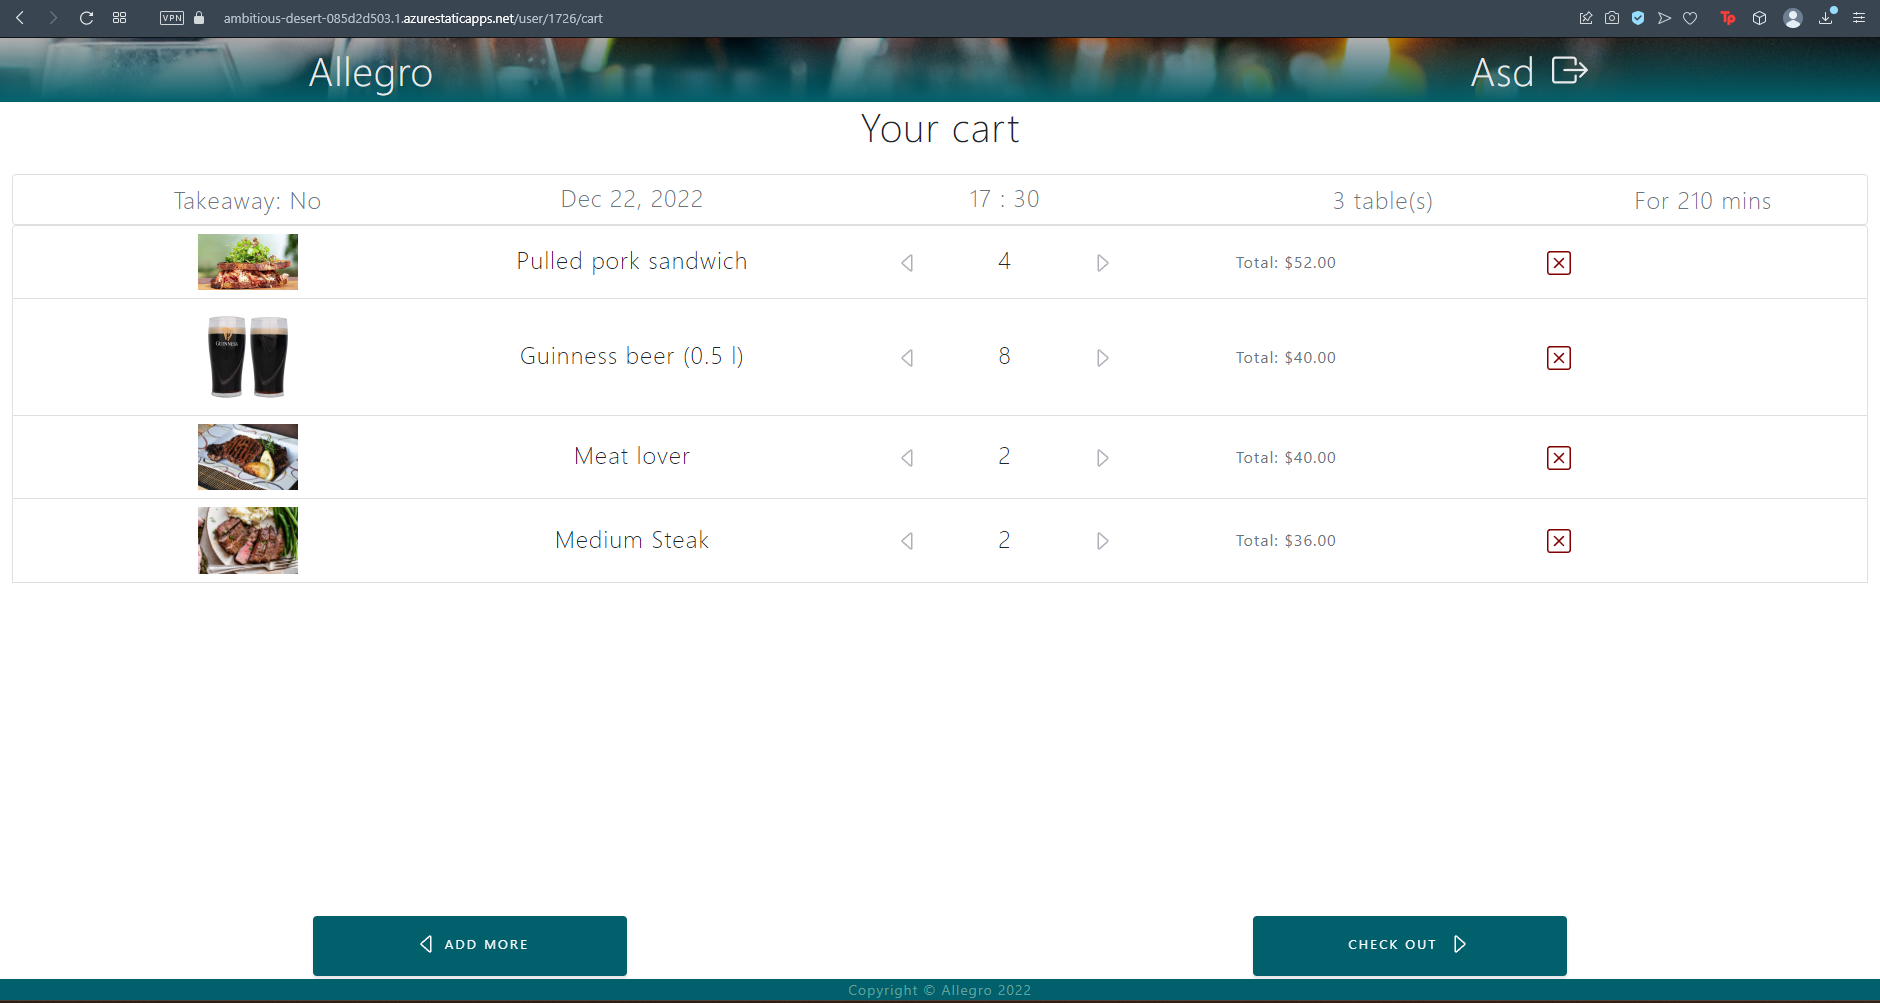
\includegraphics[width=150mm, keepaspectratio]{figures/UI/3_Cart.png}
\caption{Cart component UI} 
\label{fig:UI_3}
\end{figure}

\begin{figure}[ht]
	\centering
	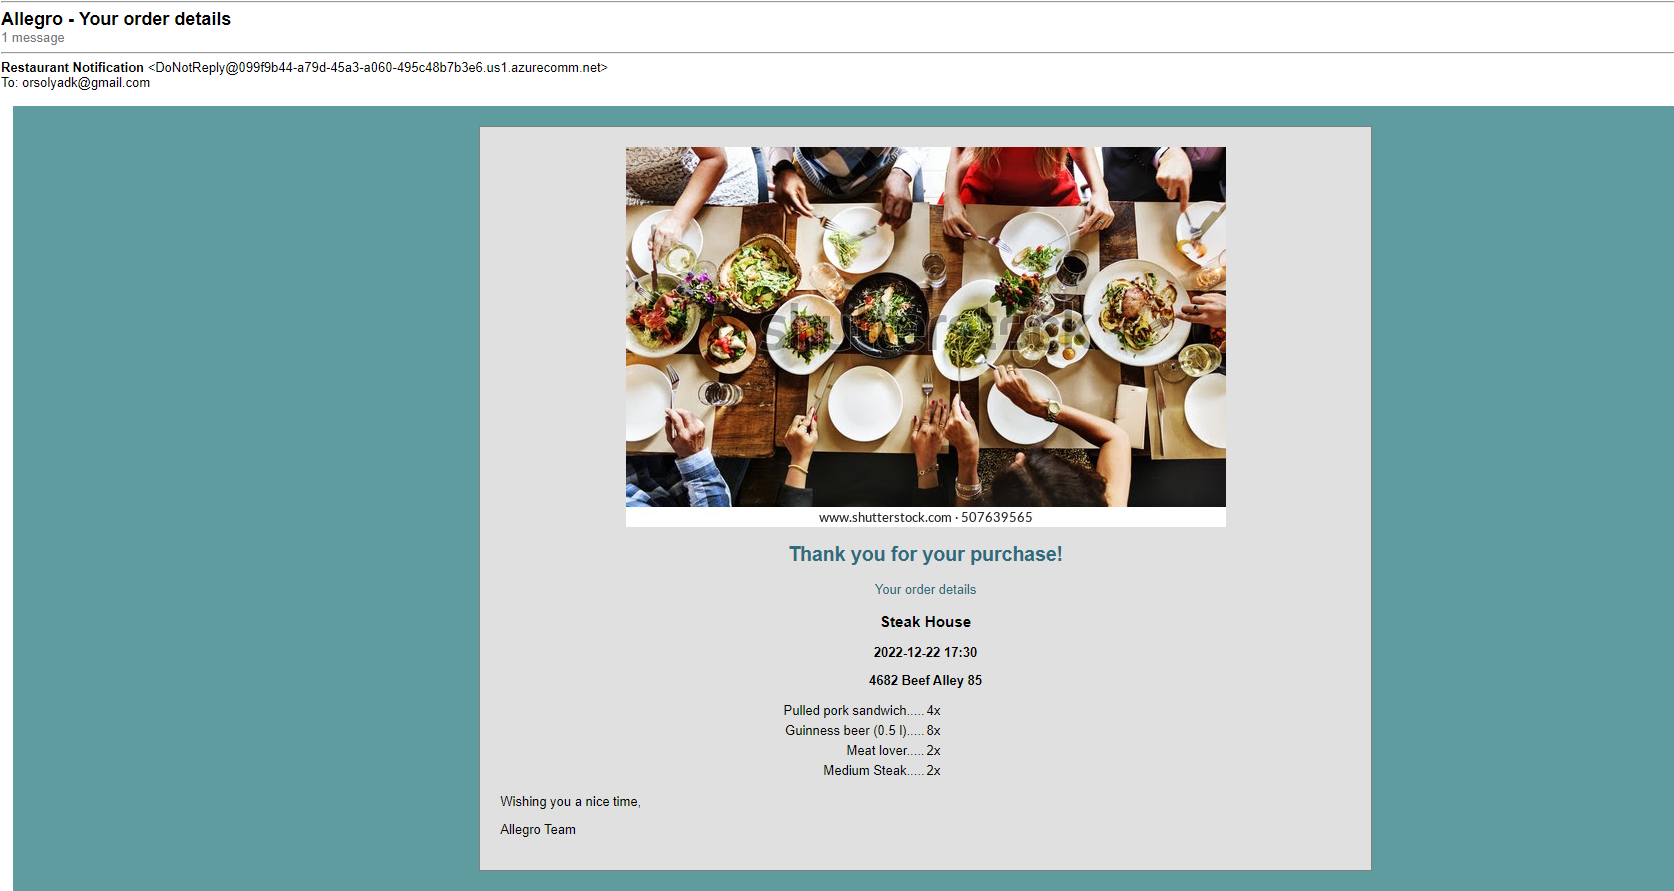
\includegraphics[width=150mm, keepaspectratio]{figures/UI/7_Email_1.png}
	\caption{Sent e-mails} 
	\label{fig:UI_6}
\end{figure}

\begin{figure}[ht]
	\centering
	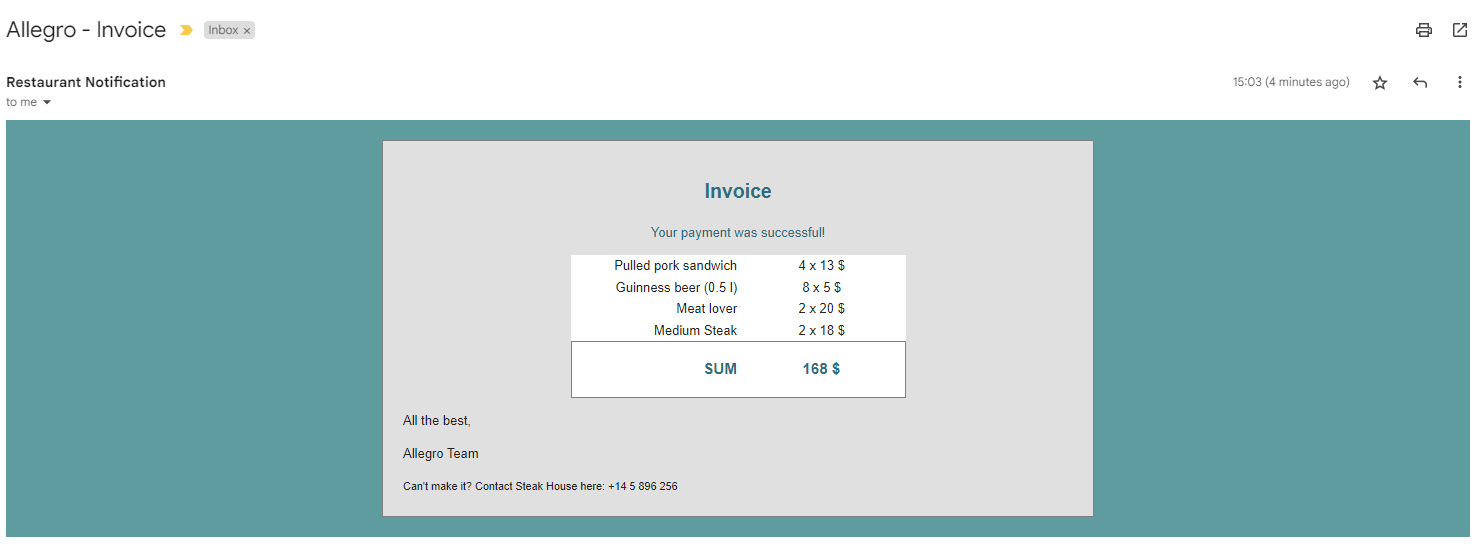
\includegraphics[width=150mm, keepaspectratio]{figures/UI/7_Email_2.png}
	\caption{Sent e-mails} 
	\label{fig:UI_7}
\end{figure}

\begin{figure}[ht]
	\centering
	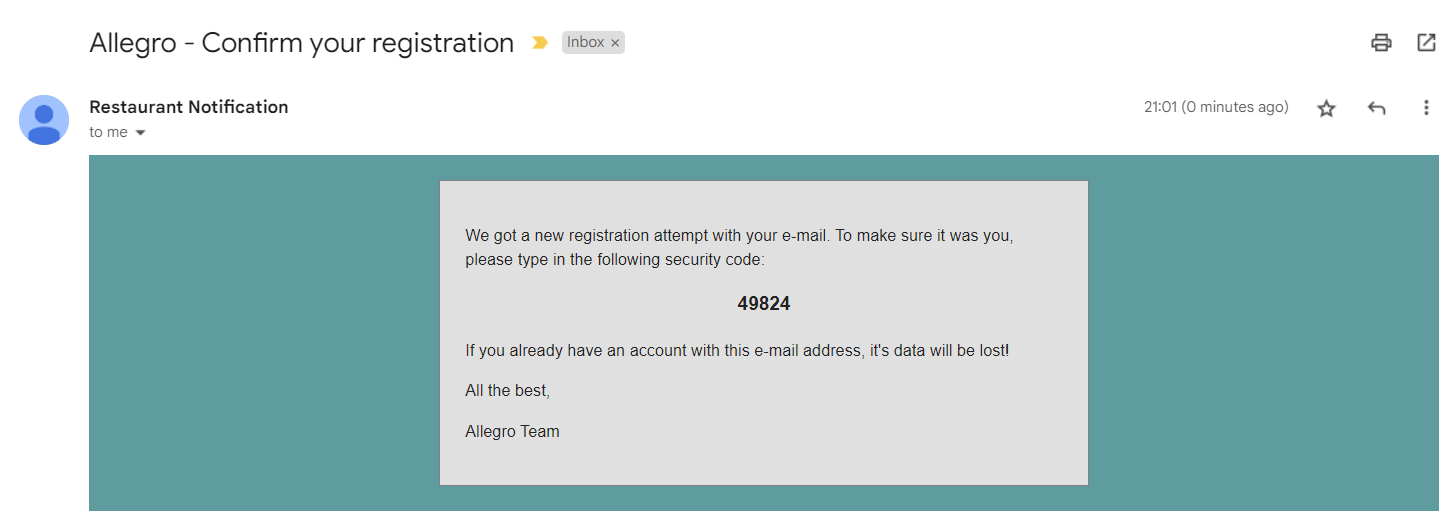
\includegraphics[width=150mm, keepaspectratio]{figures/UI/7_Email_3.png}
	\caption{Sent e-mails} 
	\label{fig:UI_7.1}
\end{figure}

\begin{figure}[ht]
	\centering
	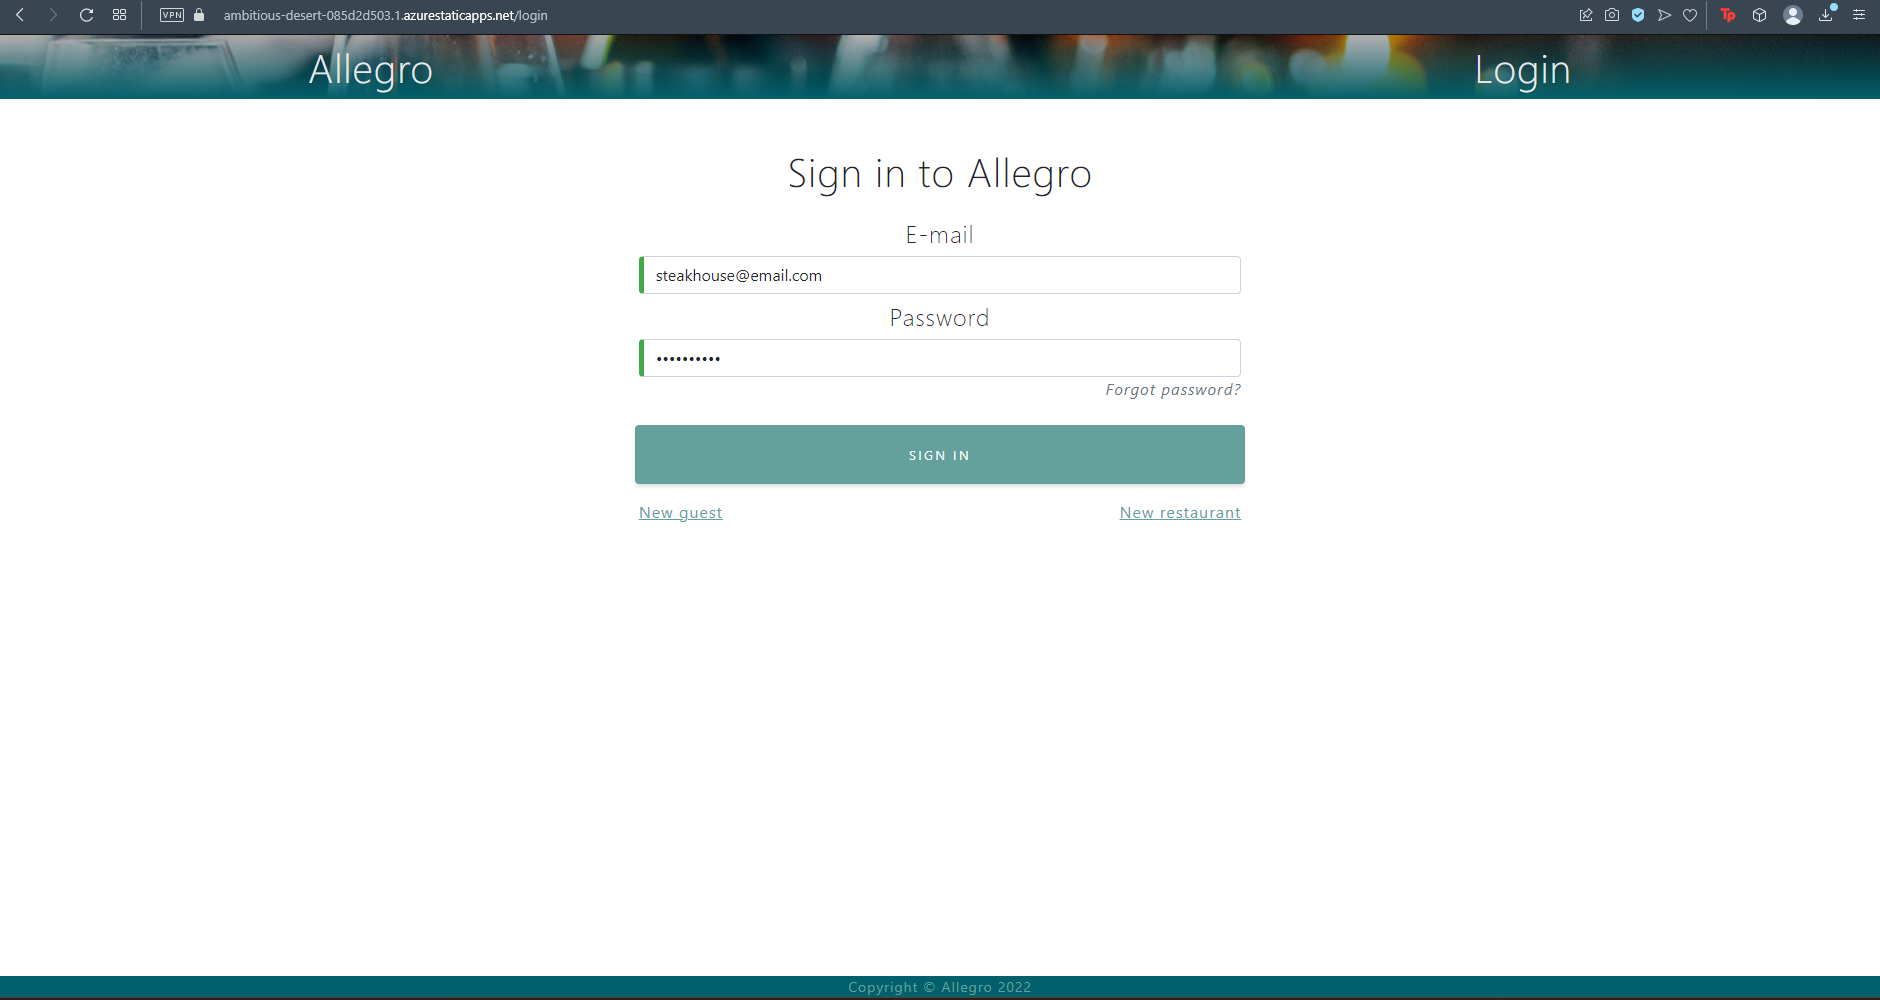
\includegraphics[width=150mm, keepaspectratio]{figures/UI/8_Login.png}
	\caption{Login component UI} 
	\label{fig:UI_8}
\end{figure}

\begin{figure}[ht]
	\centering
	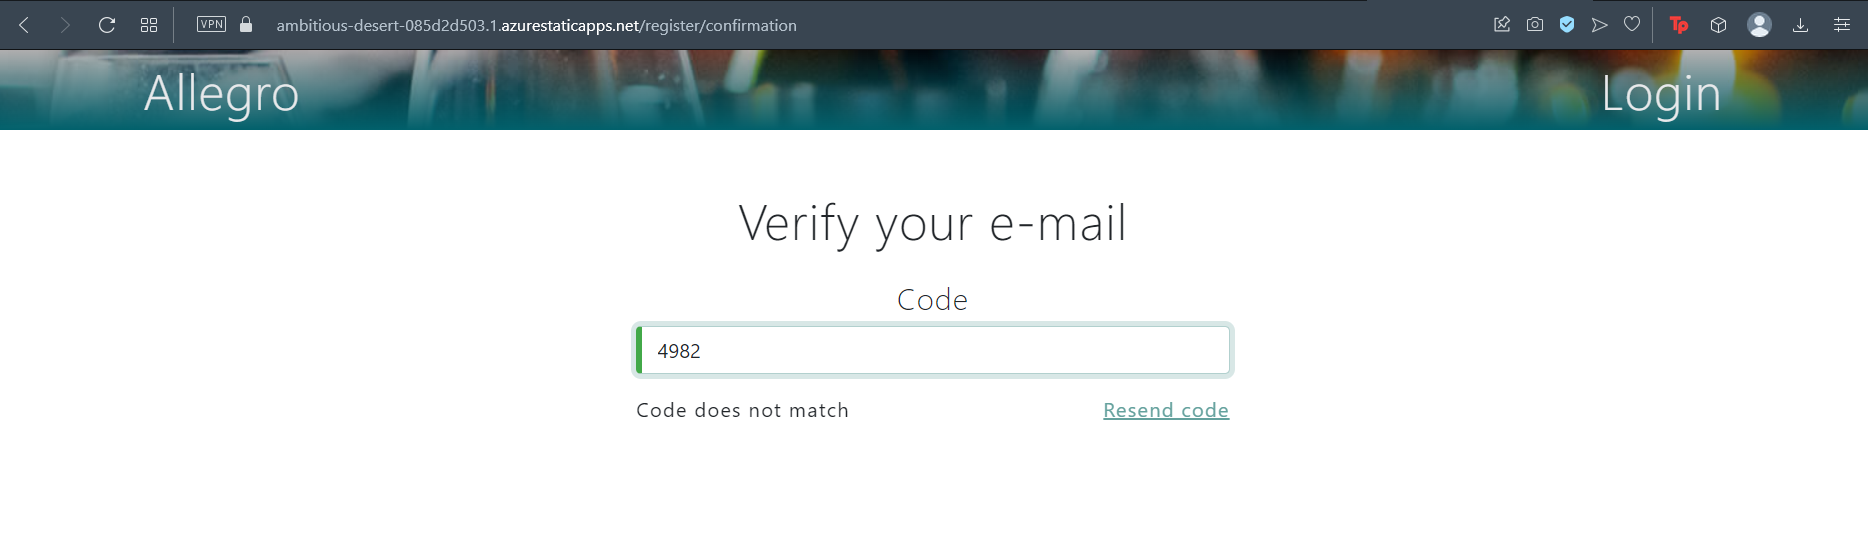
\includegraphics[width=150mm, keepaspectratio]{figures/UI/8_ConfirmFalse.png}
	\caption{Wrong confirmation code} 
	\label{fig:UI_8.2}
\end{figure}

\begin{figure}[ht]
	\centering
	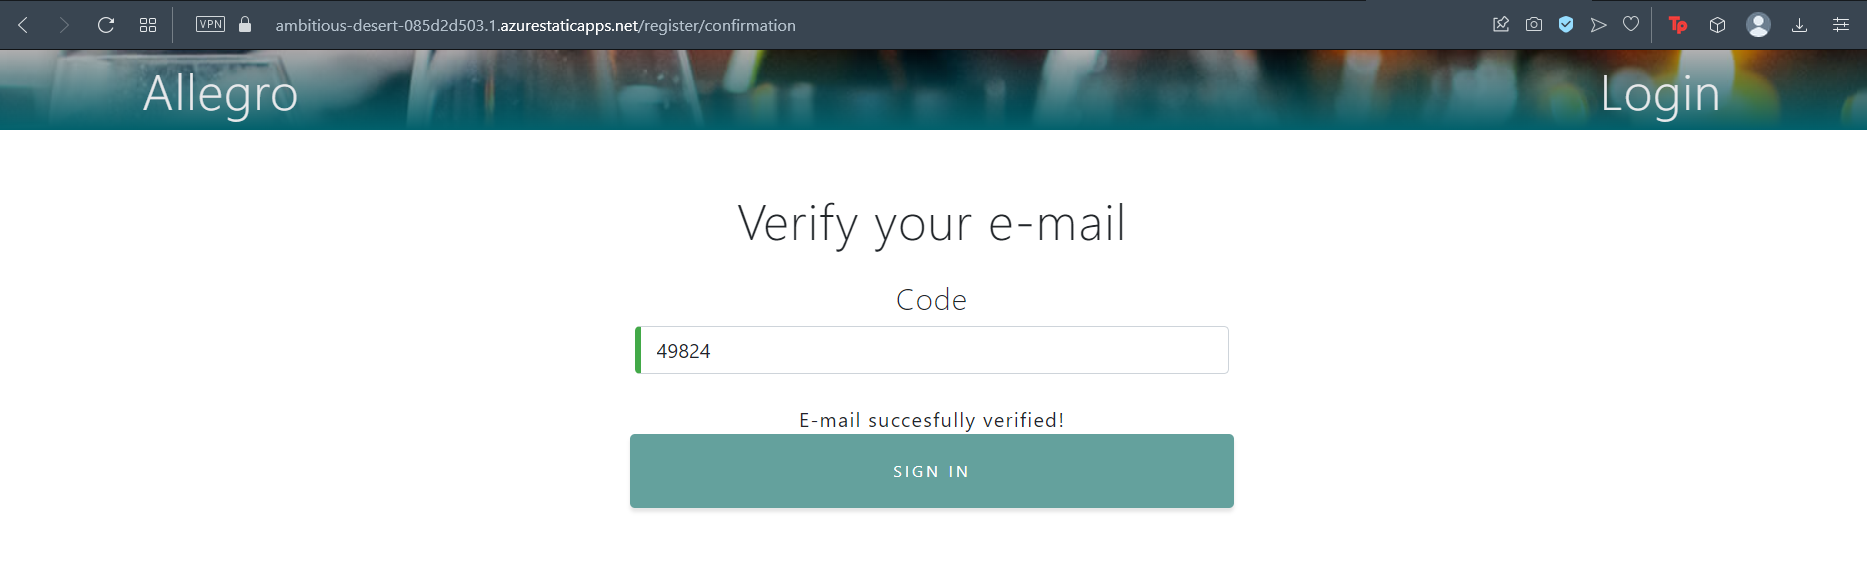
\includegraphics[width=150mm, keepaspectratio]{figures/UI/8_ConfirmSuccess.png}
	\caption{Successful confirmation} 
	\label{fig:UI_8.3}
\end{figure}

\begin{figure}[ht]
	\centering
	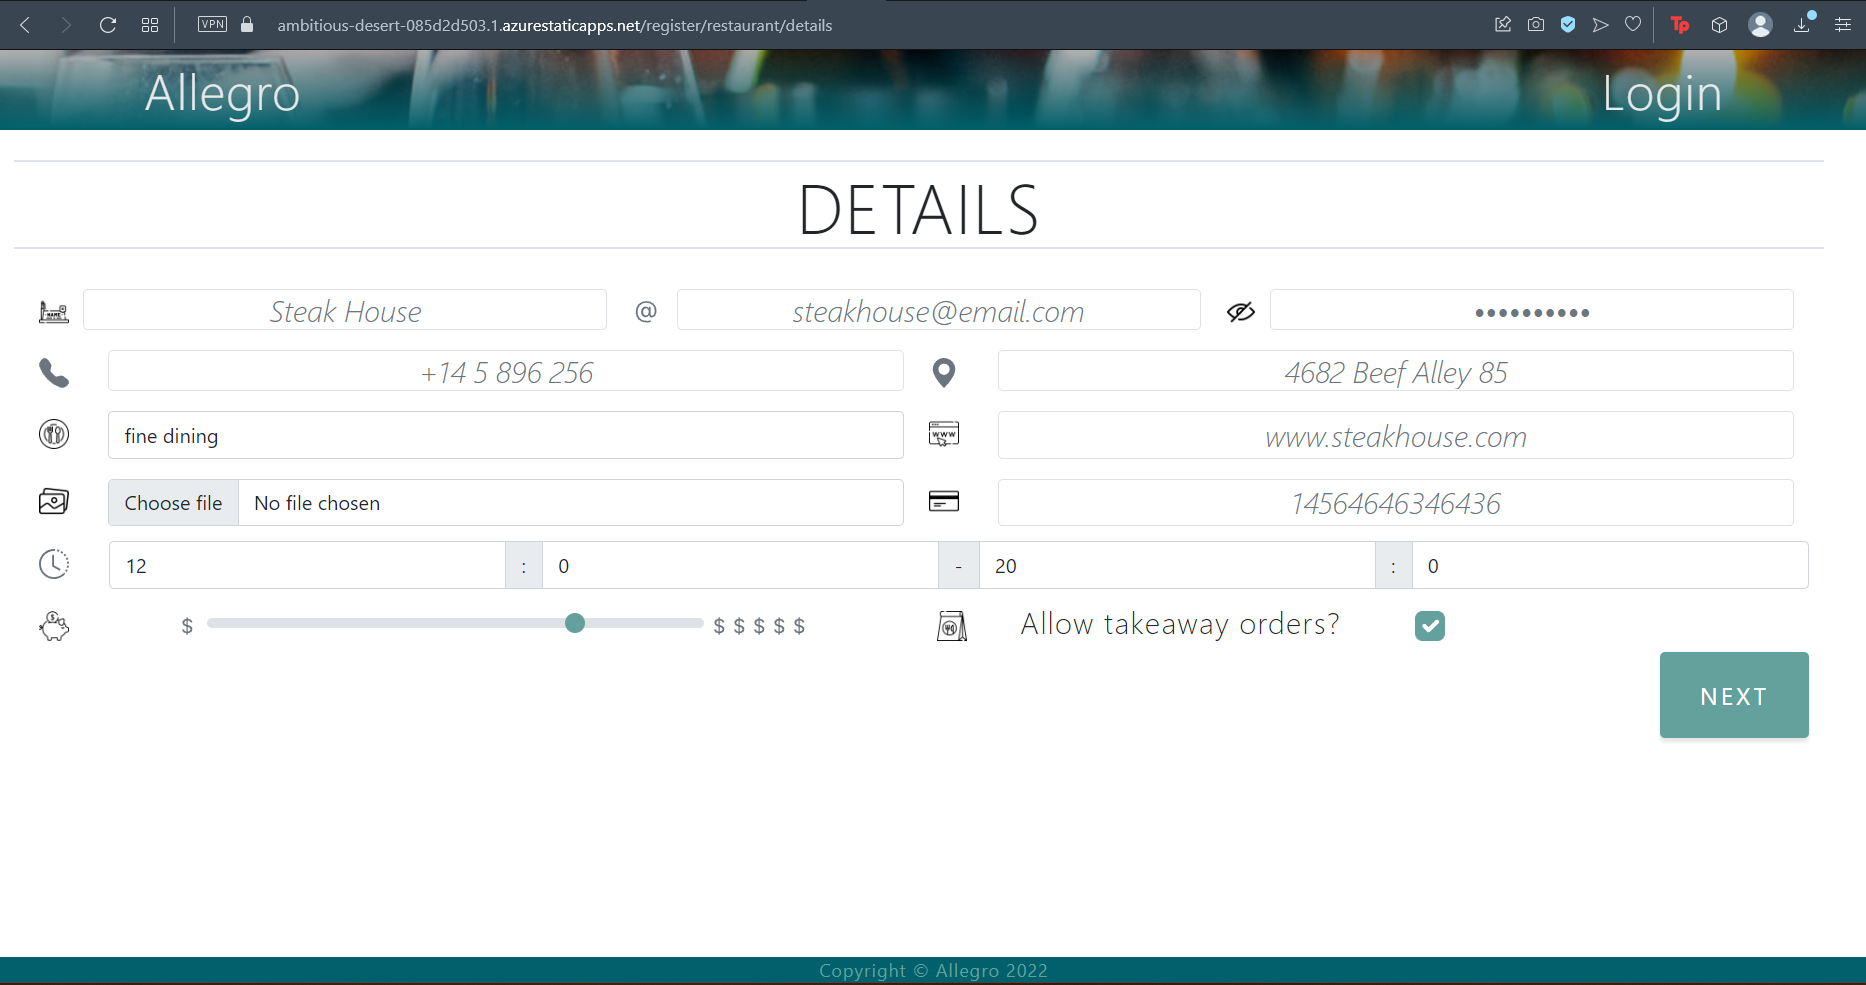
\includegraphics[width=150mm, keepaspectratio]{figures/UI/9_RestaurantDetailsEdit.png}
	\caption{Restaurant details registration UI} 
	\label{fig:UI_9}
\end{figure}

\begin{figure}[ht]
	\centering
	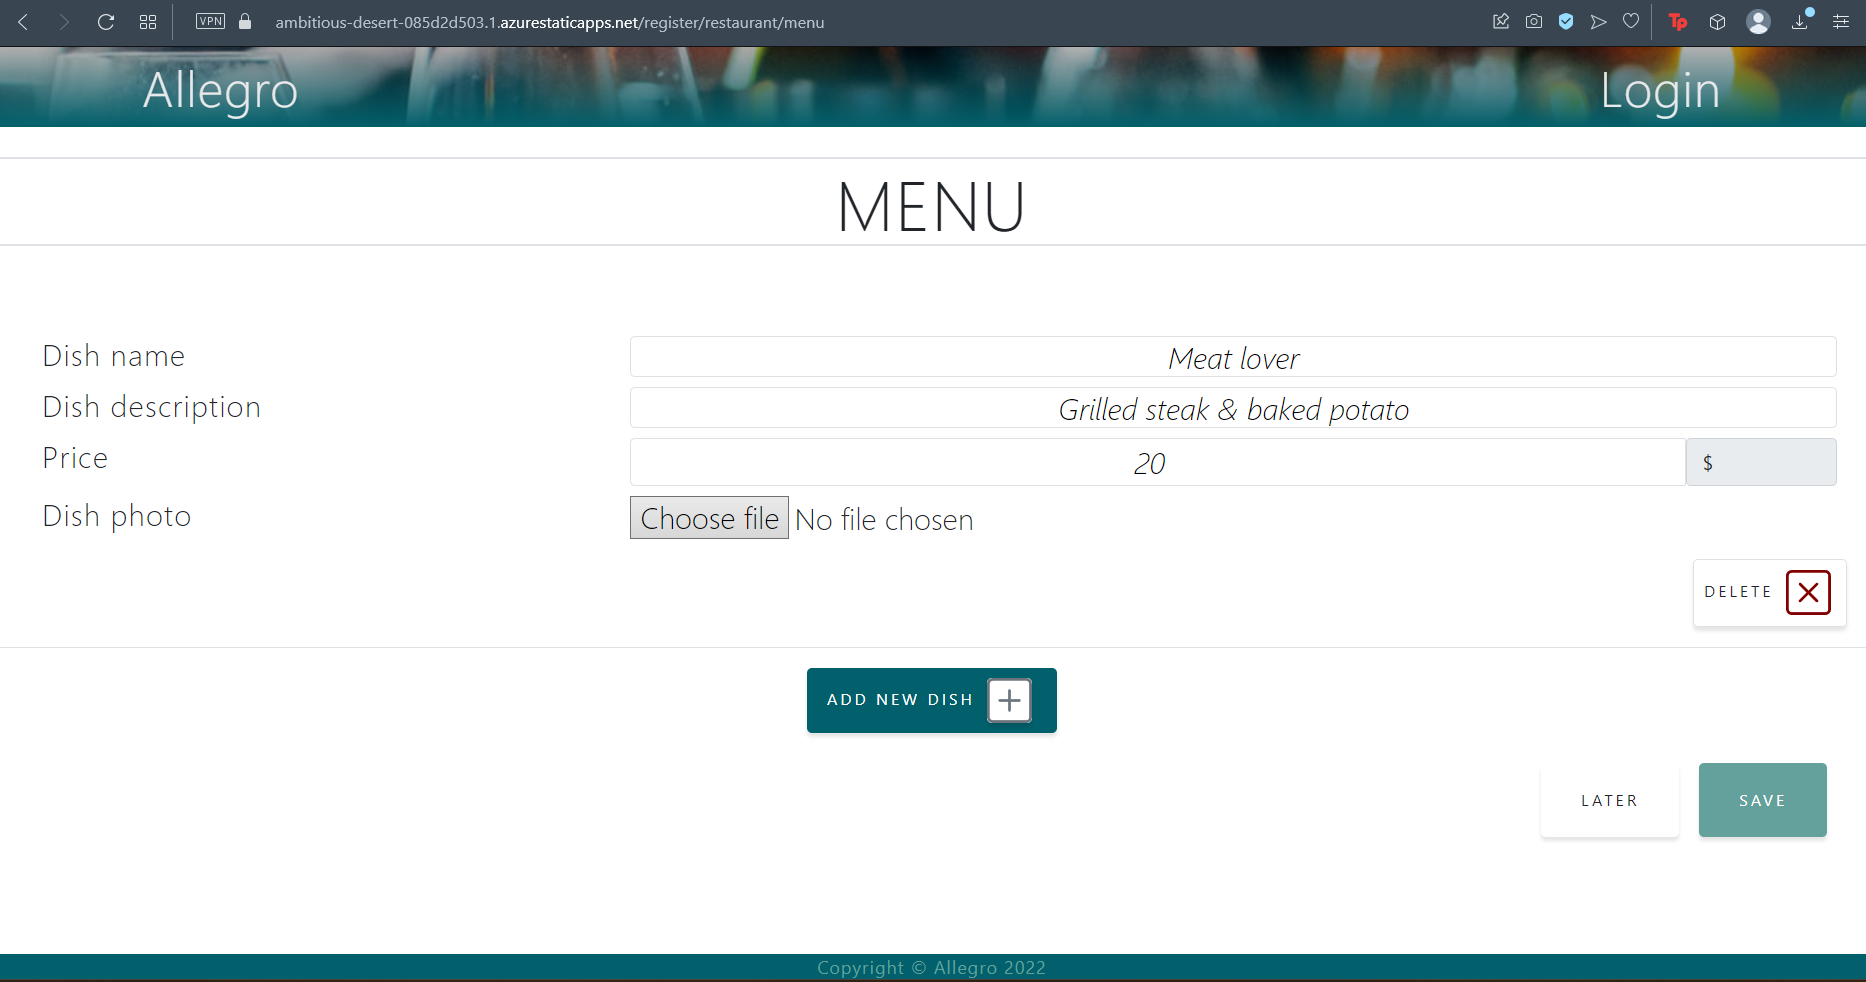
\includegraphics[width=150mm, keepaspectratio]{figures/UI/10_RestaurantMenuEdit.png}
	\caption{Restaurant menu registration UI} 
	\label{fig:UI_10}
\end{figure}

\begin{figure}[ht]
	\centering
	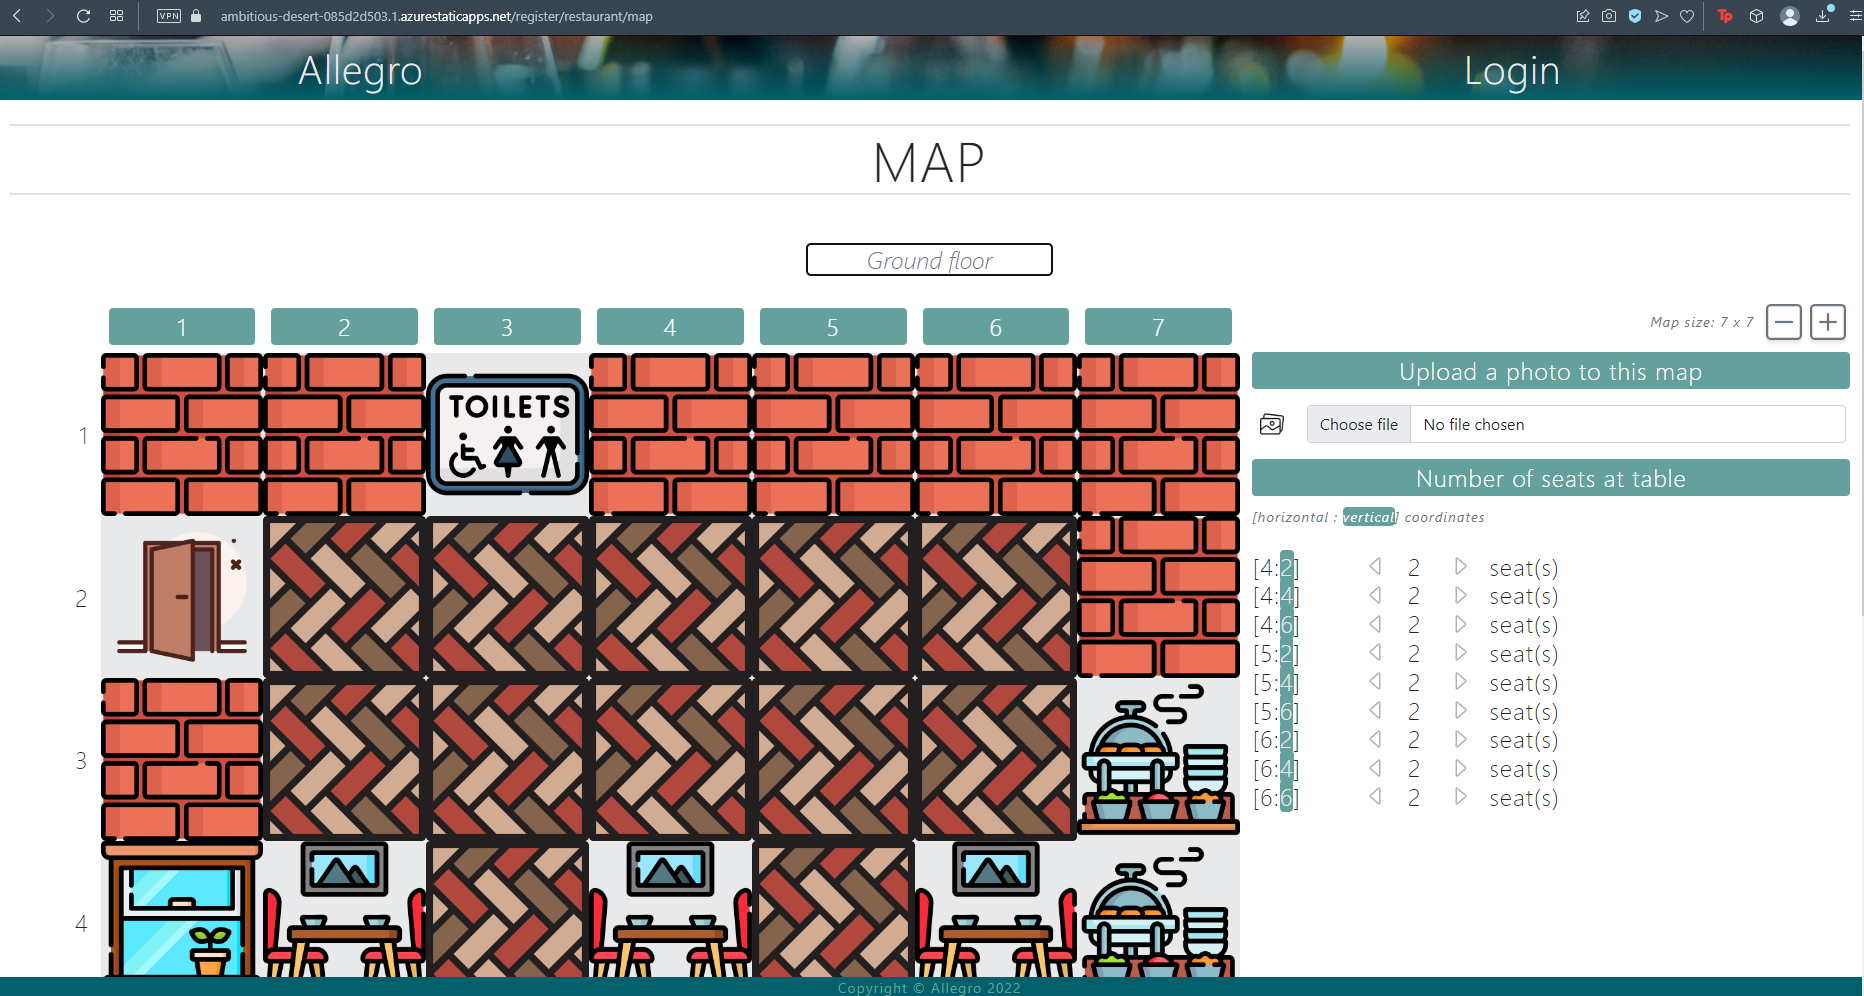
\includegraphics[width=150mm, keepaspectratio]{figures/UI/11_RestaurantMapEdit.png}
	\caption{Restaurant map registration UI} 
	\label{fig:UI_11}
\end{figure}

\begin{figure}[ht]
	\centering
	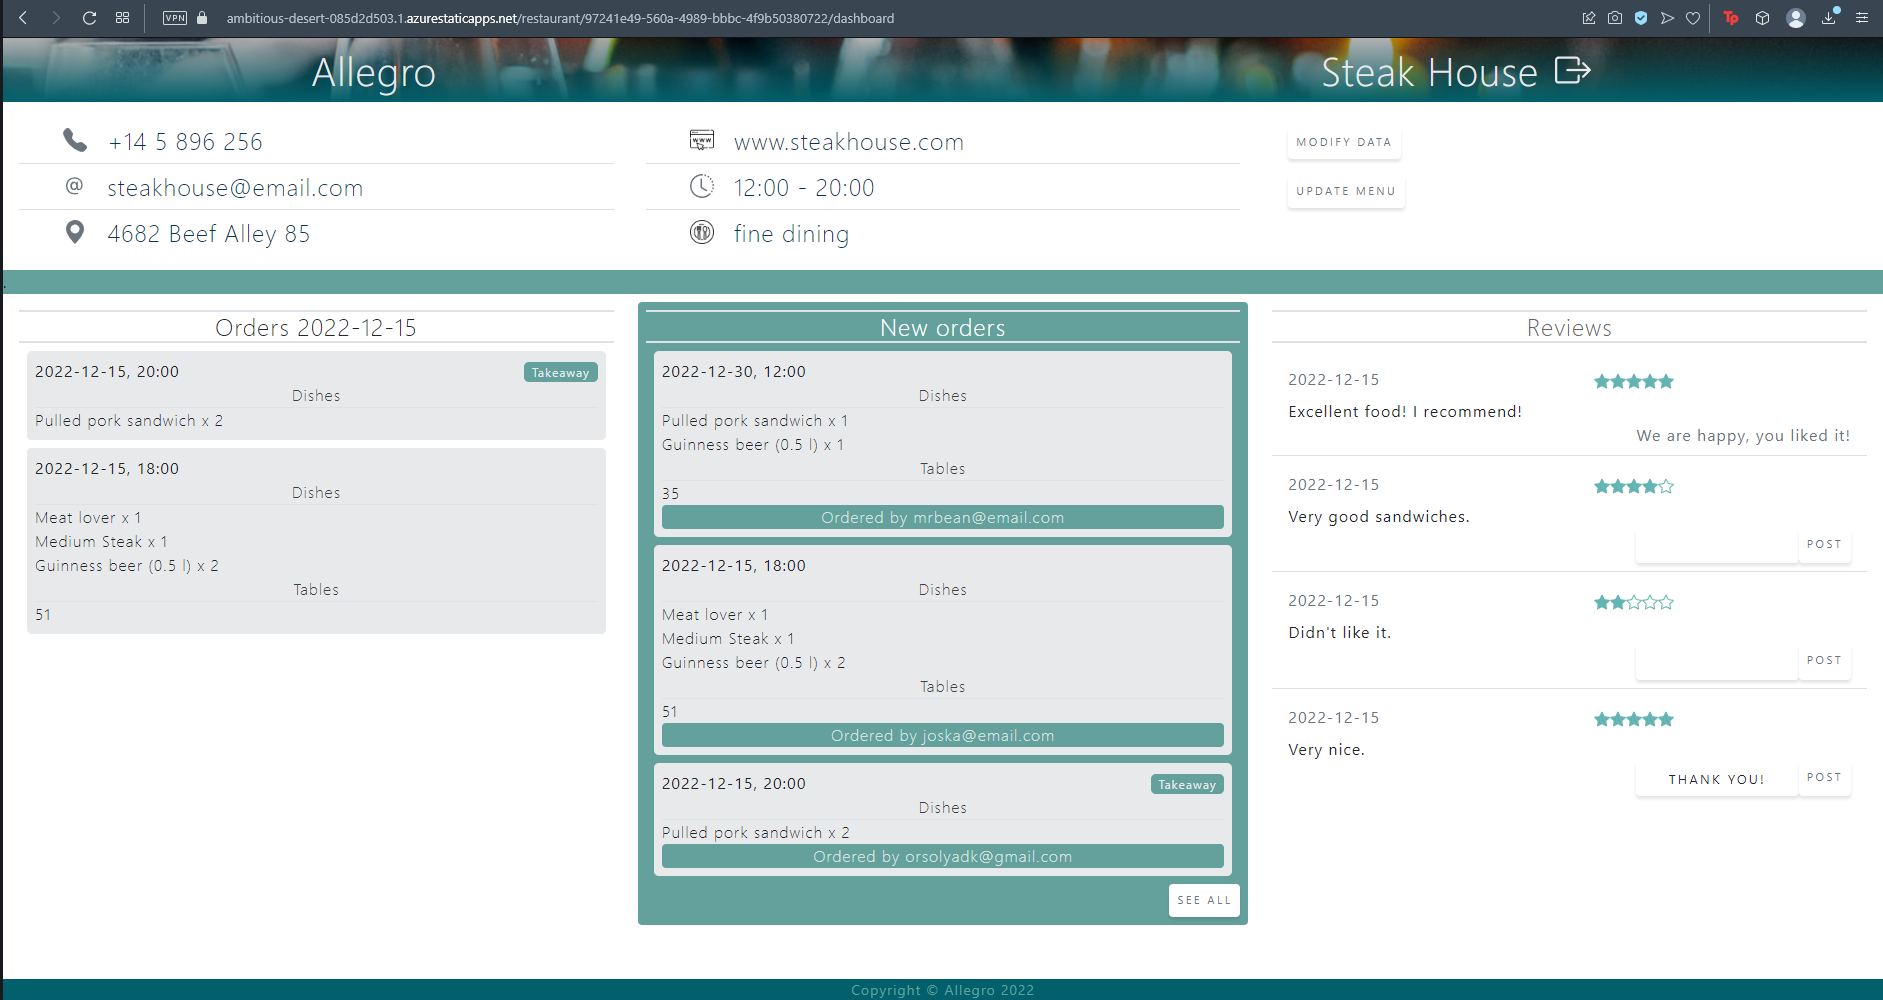
\includegraphics[width=150mm, keepaspectratio]{figures/UI/12_Dashboard.png}
	\caption{Restaurant dashboard UI} 
	\label{fig:UI_12}
\end{figure}

\begin{figure}[ht]
	\centering
	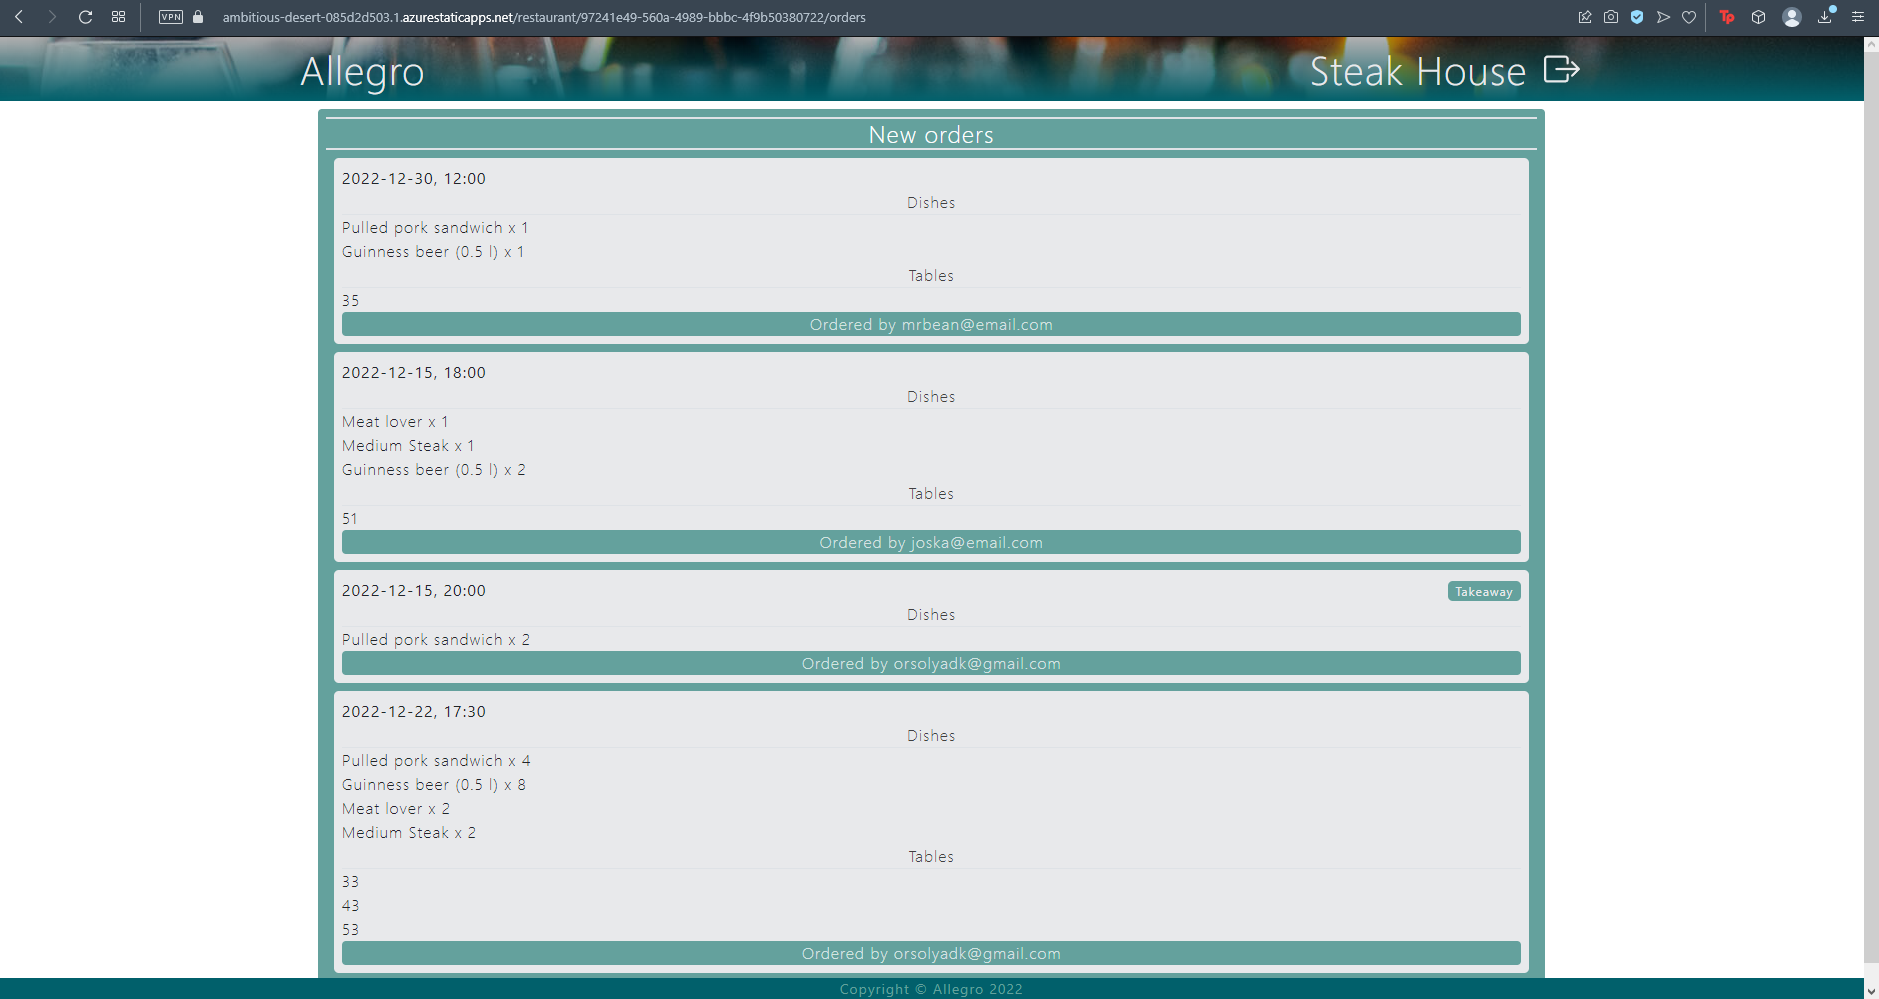
\includegraphics[width=150mm, keepaspectratio]{figures/UI/13_Orders.png}
	\caption{Restaurant all orders UI} 
	\label{fig:UI_13}
\end{figure}

\begin{figure}[ht]
	\centering
	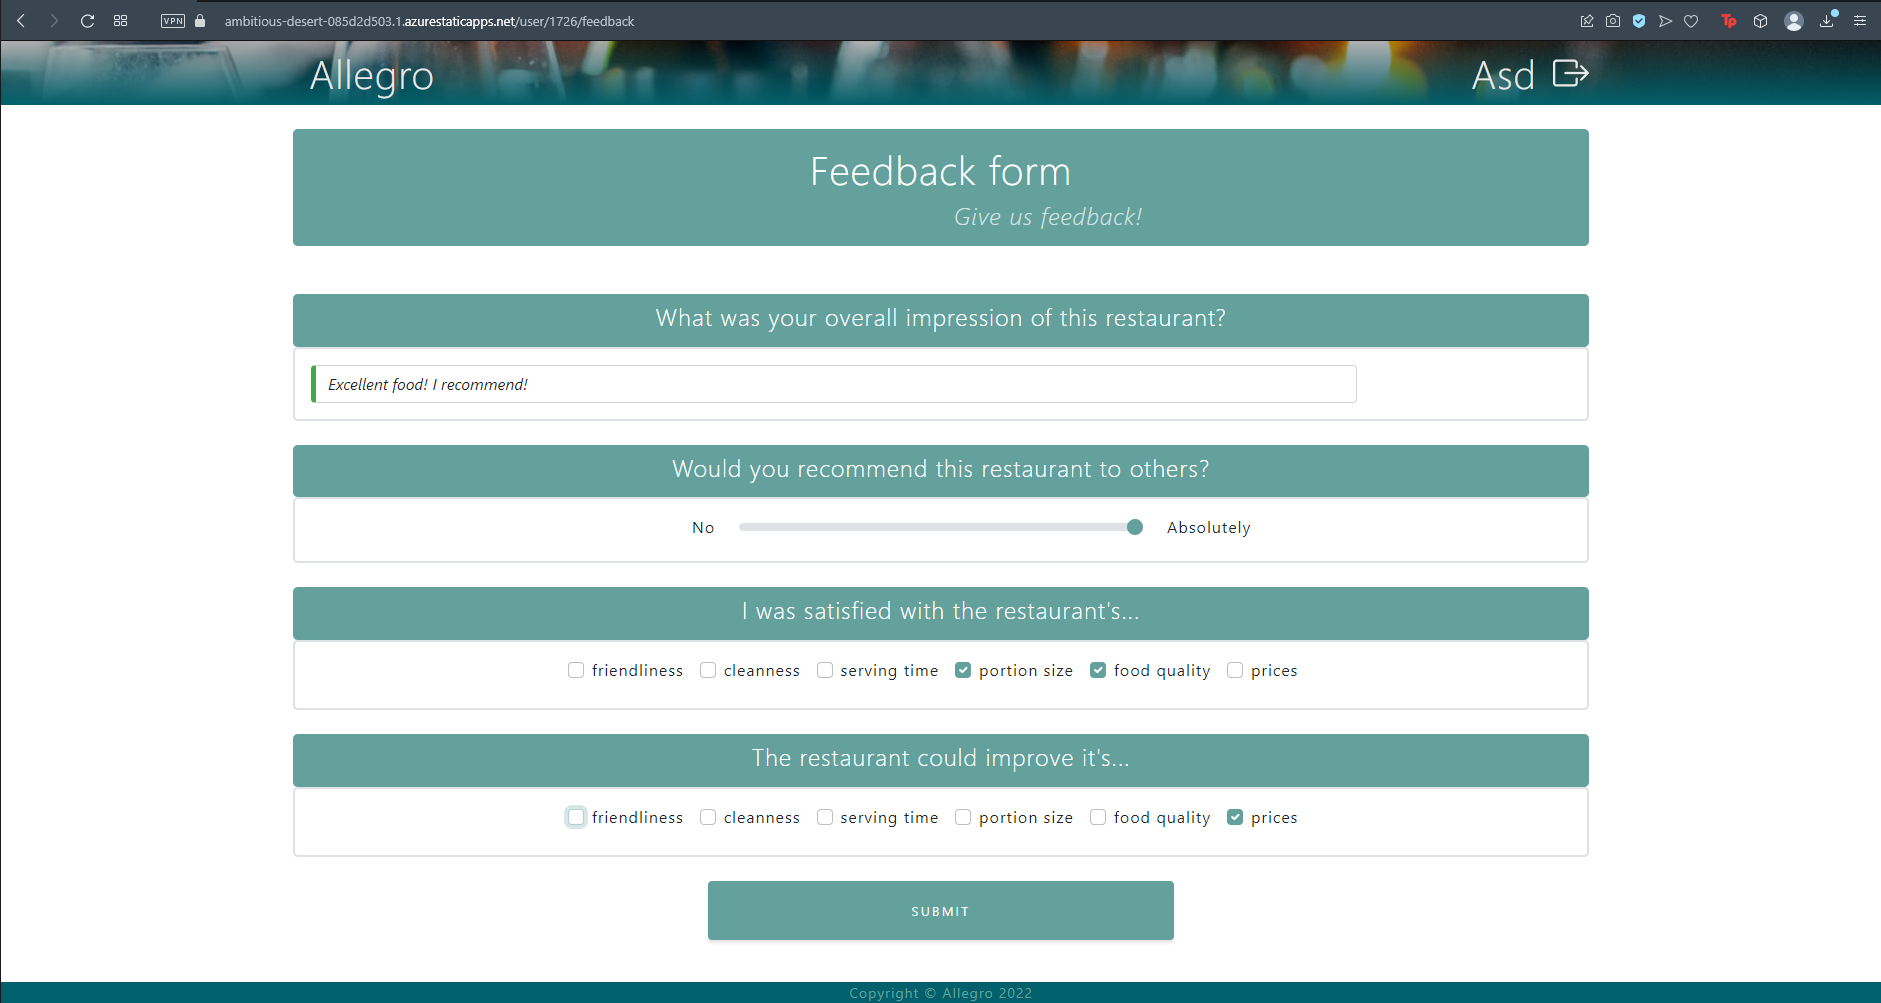
\includegraphics[width=150mm, keepaspectratio]{figures/UI/14_Feedback.png}
	\caption{Feedback component UI} 
	\label{fig:UI_14}
\end{figure}

\label{page:last}
\end{document}
